%% http://user.uni-frankfurt.de/~muehlich/tex/wordvslatex.html
 % Local variables:
 % TeX-open-quote: "\"`"
 % TeX-close-quote: "\"'"
 % End:

%% Um in Bibliographie dt. Titel von \MakeSentenceCase zu schuetzen, doppelte {{}} verwenden.


%%global serifenlos einstellen: \renewcommand*\familydefault{\sfdefault}


\documentclass[%
handout%
]{beamer}\usepackage{graphicx, color}
%% maxwidth is the original width if it is less than linewidth
%% otherwise use linewidth (to make sure the graphics do not exceed the margin)
\makeatletter
\def\maxwidth{ %
  \ifdim\Gin@nat@width>\linewidth
    \linewidth
  \else
    \Gin@nat@width
  \fi
}
\makeatother

\IfFileExists{upquote.sty}{\usepackage{upquote}}{}
\definecolor{fgcolor}{rgb}{0.2, 0.2, 0.2}
\newcommand{\hlnumber}[1]{\textcolor[rgb]{0,0,0}{#1}}%
\newcommand{\hlfunctioncall}[1]{\textcolor[rgb]{0.501960784313725,0,0.329411764705882}{\textbf{#1}}}%
\newcommand{\hlstring}[1]{\textcolor[rgb]{0.6,0.6,1}{#1}}%
\newcommand{\hlkeyword}[1]{\textcolor[rgb]{0,0,0}{\textbf{#1}}}%
\newcommand{\hlargument}[1]{\textcolor[rgb]{0.690196078431373,0.250980392156863,0.0196078431372549}{#1}}%
\newcommand{\hlcomment}[1]{\textcolor[rgb]{0.180392156862745,0.6,0.341176470588235}{#1}}%
\newcommand{\hlroxygencomment}[1]{\textcolor[rgb]{0.43921568627451,0.47843137254902,0.701960784313725}{#1}}%
\newcommand{\hlformalargs}[1]{\textcolor[rgb]{0.690196078431373,0.250980392156863,0.0196078431372549}{#1}}%
\newcommand{\hleqformalargs}[1]{\textcolor[rgb]{0.690196078431373,0.250980392156863,0.0196078431372549}{#1}}%
\newcommand{\hlassignement}[1]{\textcolor[rgb]{0,0,0}{\textbf{#1}}}%
\newcommand{\hlpackage}[1]{\textcolor[rgb]{0.588235294117647,0.709803921568627,0.145098039215686}{#1}}%
\newcommand{\hlslot}[1]{\textit{#1}}%
\newcommand{\hlsymbol}[1]{\textcolor[rgb]{0,0,0}{#1}}%
\newcommand{\hlprompt}[1]{\textcolor[rgb]{0.2,0.2,0.2}{#1}}%

\usepackage{framed}
\makeatletter
\newenvironment{kframe}{%
 \def\at@end@of@kframe{}%
 \ifinner\ifhmode%
  \def\at@end@of@kframe{\end{minipage}}%
  \begin{minipage}{\columnwidth}%
 \fi\fi%
 \def\FrameCommand##1{\hskip\@totalleftmargin \hskip-\fboxsep
 \colorbox{shadecolor}{##1}\hskip-\fboxsep
     % There is no \\@totalrightmargin, so:
     \hskip-\linewidth \hskip-\@totalleftmargin \hskip\columnwidth}%
 \MakeFramed {\advance\hsize-\width
   \@totalleftmargin\z@ \linewidth\hsize
   \@setminipage}}%
 {\par\unskip\endMakeFramed%
 \at@end@of@kframe}
\makeatother

\definecolor{shadecolor}{rgb}{.97, .97, .97}
\definecolor{messagecolor}{rgb}{0, 0, 0}
\definecolor{warningcolor}{rgb}{1, 0, 1}
\definecolor{errorcolor}{rgb}{1, 0, 0}
\newenvironment{knitrout}{}{} % an empty environment to be redefined in TeX

\usepackage{alltt}



\usepackage[T1]{fontenc}
\usepackage[utf8]{inputenc}

\usepackage[ngerman]{babel}


\usepackage[seriftt]{lucidabr}
\let\digamma\relax %% muss vor lucimatx stehen; Quelle: http://article.gmane.org/gmane.comp.tex.german/11025
%\usepackage{lucimatx}
%\usepackage{helvet}

%\usepackage{color}
\usepackage{enumerate}
%\usepackage{pifont}
\usepackage[geometry]{ifsym}

\usepackage{graphicx}
\graphicspath{{fig/}}

\usepackage{colortbl}

%\usepackage{multirow}
\usepackage{booktabs}
\usepackage{tabularx}
\usepackage{rccol}
\usepackage{dcolumn}
\usepackage{numprint}


\usepackage{hyperref}

\usepackage{amsmath}

\usepackage[normalem]{ulem}

%% Reduce spacing in table of contents (beamer)
%% http://tex.stackexchange.com/questions/51452/reduce-spacing-in-table-of-contents-beamer
\usepackage{etoolbox}
\makeatletter
\patchcmd{\beamer@sectionintoc}{\vskip1.0em}{\vskip0.3em}{}{}
\makeatother

\usepackage{listings}
%\lstset{language =[LaTeX]TeX, numbers=left, numberstyle=\tiny, stepnumber=1, numbersep=5pt,%%
%  keywordstyle=\color{red}\bfseries,showstringspaces=true}
  %% \lstset{}

\usepackage[babel,german=quotes]{csquotes}

\usepackage[style=apa, backend=biber, natbib=true, bibencoding=utf8]{biblatex}
\DeclareLanguageMapping{ngerman}{ngerman-apa}
\DeclareCaseLangs*{ngerman}
\DeclareFieldFormat{titlecase}{#1}

\addbibresource{references.bib}

%% http://www.mrunix.de/forums/showthread.php?t=67386
\DefineBibliographyStrings{ngerman}{andothers={et\addabbrvspace al\adddot}}

\usepackage{tikz}
\usetikzlibrary{positioning,mindmap,trees,shapes,shadows,calc,arrows,automata,decorations.text}

\usepackage{cclicenses}

\usepackage{fp}

\usepackage{dirtree}

\setlength{\itemsep}{2\baselineskip}

\newcommand{\myhref}[2]{\textcolor{blue}{\underline{\href{#1}{#2}}}}




\definecolor{lightblue}{rgb}{0.8,0.85,1}
\newcommand{\package}[1]{\textcolor{green}{\texttt{#1}}}
\newcommand{\argmt}[1]{\textcolor{lightblue}{\texttt{#1}}}
\newcommand{\cmnd}[1]{\colorbox{lightblue}{\lstinline|#1|}}

\newcommand{\rcode}{\vspace{2ex}\hrulefill{} Berechnung mit R \hrulefill{}}

\lstdefinestyle{inline}{basicstyle=\ttfamily, fontadjust=true}
\newcommand{\code}[1]{\lstinline[style=inline]|#1|}

\newcommand{\eCell}[1]{\multicolumn{#1}{c}{}}
\newcommand{\colHeader}[1]{\multicolumn{1}{c}{#1}}
\newcommand{\colhead}[1]{\multicolumn{1}{c}{#1}}



\newcommand{\prozeff}[1]{\FPeval\result{round(((exp(#1)-1)*100):0)}$\FPprint\result\,\%$}

\newcommand{\file}[1]{\emph{#1}}

\urlstyle{sf}

\newcommand{\inout}[3]{
  \begin{columns}
    \begin{column}{#1\textwidth}
      \lstinputlisting{#3}
    \end{column}
    \hspace{1ex}\vrule \hspace{1ex}
    \begin{column}{#2\textwidth}
      \input{#3}
    \end{column}
  \end{columns}
}


\newenvironment{itemize*}%
{\begin{itemize}%
    \setlength{\itemsep}{10pt}%
    \setlength{\parskip}{0pt}}%
   {\end{itemize}}

\newenvironment{enumerate*}%
{\begin{enumerate}%
    \setlength{\itemsep}{2ex}%
    \setlength{\parskip}{0pt}}%
   {\end{enumerate}}



\AtBeginSection[] % Do nothing for \section*
{
  \begin{frame}[plain]%<beamer>
    \frametitle{Kapitelübersicht}
    \begin{footnotesize}
      \tableofcontents[sectionstyle=show/shaded, subsectionstyle = show/show/shaded,  subsubsectionstyle=show/hide/hide]
    \end{footnotesize}
  \end{frame}
}


\AtBeginSubsection[] % Do nothing for \section*
{
  \begin{frame}[plain]%<beamer>
    \frametitle{Abschnittsübersicht}
    \begin{footnotesize}
      %%\tableofcontents[sectionstyle=show/hide, subsectionstyle = show/show/hide]
      \tableofcontents[sectionstyle=show/shaded, subsectionstyle = show/shaded/hide]
       \end{footnotesize}
  \end{frame}
}

%%\usecolortheme{beetle}
%%\useoutertheme{infolines}
%%\useinnertheme{circles}
%%\setbeamertemplate{itemize item}[circle]

\setbeamercovered{transparent}
%% Abbildungen und Tabellen numerieren
\setbeamertemplate{caption}[numbered]
\usetheme[wiso]{UzK}

\usepackage{helvet}
\setbeamerfont*{frametitle}{series = \bfseries, size = \Large}
\setbeamerfont*{title}{series = \bfseries, size = \Large}


% \hypersetup{%
%   pdftitle={Paarkonflikte, Kommunikation und die Stabilität von Partnerschaften},%
%   pdfauthor={Bernd Weiß}}

\title[]{\large{GESIS Workshop \newline\newline Grundlagen\\ sozialwissenschaftlicher\\ Meta-Analysen}}
\date{13.\,/\,14. Dezember 2012}
\author[Dr.\,Bernd Weiß, Prof.\,Dr.\,Michael Wagner]{Dr.\,Bernd Weiß \\ Prof.\,Dr.\,Michael Wagner}

\institute[Universität zu Köln]{
  Forschungsinstitut für Soziologie\\
  Universität zu Köln\\ \vspace{2ex}
  \url{bernd.weiss@uni-koeln.de}\\
  \url{mwagner@wiso.uni-koeln.de}\\
  }

% Other options:
%	style=numeric-comp,    % [1-3, 7, 8]
%	style=alphabetic,      % [Doe92; Doe95; Jon98]

% \ExecuteBibliographyOptions{
%   sorting=nty, % Sort by name, title, year.
%   % (bibtex, biber)
%   bibwarn=true, %
%   bibencoding=ascii, % (auto, ascii, inputenc, <encoding>)
%   isbn=false,%
%   url=false,%
%   doi=false,%
%   eprint=false,%
%   firstinits=true,% Initialien Erzeugen
% }%

% Nach Fertigstellung
% \input{biblatex-alpha.tex}






\begin{document}


\begin{frame}[plain]
\titlepage
\begin{flushright}
  \byncsa
\end{flushright}
\end{frame}


\part{Übersicht und Vorbemerkungen}\label{part:uebersicht}
\frame{\partpage}


\begin{frame}
  \frametitle{Ziele des Workshops}
  %%
  \begin{enumerate}
  \item Zentrale meta-analytische Konzepte und Ablauf einer Meta-Analyse verstanden haben.
  \item Publizierte Meta-Analysen nachvollziehen und kritisch beurteilen können.
  \item Vorgehen und Aufwand einer eigenen Meta-Analyse einschätzen können.
  \end{enumerate}
\end{frame}


\begin{frame}
  \frametitle{Konzeption des Workshops}
  %%
  \begin{itemize}
  \item Aufbau folgt grob dem Ablauf einer publikationsbasierten Forschungssynthese/Meta-Analyse.
  \item Mischung zwischen (Dozenten-)Vortrag und praktischen Lerneinheiten.
  \item Für die praktischen Übungen wird das Statistikpaket R benutzt (es wird
    eine kurze Einleitung geben).\footnote{Es werden aber auch
      Stata-Beispiele gezeigt.}
  \item Folien folgen nicht dem $5 \times 5$-Schema, teilweise Skriptcharakter.
  \item Übersicht statt Details.
  \item Medizinische/biostatistische Perspektive auf Meta-Analyse.
  \end{itemize}
\end{frame}


\begin{frame}
  \frametitle{Materialien des Workshops}
  \begin{itemize}
  \item Alle Materialien lassen sich von der folgenden Website herunterladen: \url{http://www.berndweiss.net/teaching.html}.
  \item Alle Materialien stehen unter einer Creative Commons
    \href{http://creativecommons.org/licenses/by-nc-sa/3.0/de/deed.en}{Attribution-NonCommercial-ShareAlike
      3.0 Germany} Lizenz.
  \item Die Verzeichnisstruktur ist wie folgt:
  \end{itemize}
    \dirtree{%
      .1 /.
      .2 assign\DTcomment{Unterlagen für Übungen}.
      .2 data\DTcomment{Alle Datensätze}.
      .2 fig\DTcomment{Abbildungen}.
      .2 org\DTcomment{(Öffentliche) Orga-Materialien}.
      .2 ref\DTcomment{Literatur (PDFs)}.
      .2 slide\DTcomment{Folien des Workshops}.
      .2 src\DTcomment{R- und Stata-Analysecode}.
      .2 tab\DTcomment{Tabellen, Ausgabedateien}.
    }

\end{frame}


\begin{frame}[plain]
  \frametitle{Zeitplan Workshop Tag 1}
  \begin{center}
    \begin{tabularx}{\linewidth}{@{}rr>{\raggedright\arraybackslash}X@{}}
      \toprule
      \multicolumn{1}{c}{Zeit}  &  Dauer  &  Thema                                                                  \\
      \midrule
      10:30-12:15  &    105  &  Begrüßung, Einführung, Literaturrecherche und -organisation            \\
      12:15-13:30  &         &  \emph{Mittagspause}                                                    \\
      13:30-15:00  &     90  &  Datenerfassung, -organisation und Effektstärken I                      \\
      15:00-15:15  &         &  \emph{Pause}                                                           \\
      15:15-16:30  &     75  &  Effektstärken II und Effektstärkenverteilungen I (Fixed-effect model)  \\
      16:30-16:40  &         &  \emph{Pause}                                                           \\
      16.40-18:15  &     95  &  Einführung in R/Stata; praktische Übungen zu den bisherigen Themen     \\
      ab 18:15  &         &  Kölsch/Wine and Cheese                                                        \\
      \bottomrule
    \end{tabularx}
\end{center}
\end{frame}


\begin{frame}
  \frametitle{Zeitplan Workshop Tag 2}
  \begin{center}
    \begin{tabularx}{\linewidth}{@{}rr>{\raggedright\arraybackslash}X@{}}
      \toprule
      \multicolumn{1}{c}{Zeit}  &  Dauer  &  Thema                                                                    \\
      \midrule
      09:00-10:30  &     90  &  Effektstärkenverteilungen II (Random-effects model); praktische Übungen  \\
      10:30-10:45  &         &  \emph{Pause}                                                             \\
      10:45-12:15  &     90  &  Heterogenität, Meta-Regression, Publication bias                         \\
      12:15-13:30  &         &  \emph{Mittagspause}                                                      \\
      13:30-15:00  &     90  &  Praktische Übungen mit R/Stata                                           \\
      15:00-15:15  &         &  \emph{Pause}                                                             \\
      15.15-16.00  &     45  &  Meta-Analyse mit Individualdaten (IPD)                                   \\
      16.00-16:45  &     45  &  Fragen, Diskussion \& Feedback                                           \\
      \bottomrule
    \end{tabularx}
  \end{center}
\end{frame}




\begin{frame}[allowframebreaks]
  \frametitle{Unser Interesse an Meta-Analyse}

  \begin{footnotesize}
    \begin{itemize}
    \item \fullcite{wagner_bilanz_2003}
    \item \fullcite{wagner_meta-analyse_2006}
    \item \fullcite{wagner_variation_2006}
    \item \fullcite{weis_potentiale_2008}
    \item \fullcite{weis_meta-analyse_2008}
    \item \fullcite{weis_identification_2011}
    \item \fullcite{thompson_introduction_2013}
    \end{itemize}

    \pagebreak

    Gegenwärtige/Zukünftige Projekte:
    \begin{itemize}
    \item How employment status affects partnership stability: A meta-analysis
      using longitudinal individual person data
    \item Untersuchung zum Publication Bias am Beispiel von drei
      dt. sozialwissenschaftlichen Zeitschriften (KZfSS, PVS, ZFS)
    \item Simulationsstudie zu den Auswirkungen von unterschiedlich
      spezifizierten EHA Regressionsmodellen im Rahmen einer Meta-Analyse
    \item Fortsetzung der Meta-Analyse zur Ehescheidung
    \end{itemize}
  \end{footnotesize}

\end{frame}




%%\frame{\frametitle{Formalia}\tableofcontents[part=1]}
\frame{\frametitle{2. Einführung und Motivation}\tableofcontents[part=2]}
\frame{\frametitle{3. Forschungssynthese als sozialwissenschaftliche Methode}\tableofcontents[part=3]}
\frame[plain]{\frametitle{4. Meta-Analyse}
  \begin{footnotesize}
    \tableofcontents[part=4]
  \end{footnotesize}
}
\frame{\frametitle{5. Anhang}\tableofcontents[part=5]}



\part{Einführung}\label{part:einfuhrung}
\frame{\partpage}

\frame{\frametitle{Einführung}\tableofcontents[part=2, hideallsubsections]}


\section{Notwendigkeit von Forschungssynthesen}


\begin{frame}
  \frametitle{Gründe für die Durchführung einer Forschungssynthese}
  \begin{itemize}[<+->]
  \item Unsicherheit über die Wirksamkeit von Maßnahmen (Interventionen) (Politik, Schule, Medizin etc.).
  \item Fehlender Gesamtüberblick über einen bestimmten (wissenschaftlichen)
    Forschungsbereich, um sinnvoll weitere (methodische wie inhaltliche)
    Forschung zu initiieren.
  \item \ldots
  \end{itemize}
\end{frame}


\begin{frame}
  \frametitle{"Wächst der Wissenschaft das Wissen über den Kopf?"}
  \begin{itemize}
  \item "`But today we are experiencing a crisis of faith; many of us no longer feel sure that science, though growing
    explosively, is moving inexorably toward the truth. [\ldots] increasingly chaotic output of contemporary research"'
    (Hunt 1997: 1).
  \item "`Literaturflut - Informationslawine - Wissensexplosion. Wächst der Wissenschaft das Wissen über den Kopf?"'
    (Marx\,/\,Gramm 2002)
  \item \ldots
  \end{itemize}
\end{frame}


\begin{frame}
  \frametitle{Indikatoren für eine "`Informationslawine"' in den empirischen Sozialwissenschaften}
  \begin{itemize}[<+->]
  \item Das Kölner Zentralarchiv für empirische Sozialforschung erfasst 150 bis 200 Studien p.a. (pers. Kommunikation mit
    Oliver Watteler vom 2. Mai 2008)
  \item 120 Publikationen zum Trennungs-/Ehescheidungsrisiko in Europa (Wagner/Weiß 2006)
  \item17 Publikationen und 20 Originaldatensätze über 24 Städte in NRW zu Wanderungsmotiven (Bleck/Wagner 2006)
  \item 15 Individualdatensätze mit Angaben von \numprint{80000} Jugendlichen zum Schulschwänzen (Weiß 2008)
  \item \ldots
  \end{itemize}
\end{frame}


\begin{frame}[plain]\frametitle{Eingereichte und veröffentlichte Manuskripte in
    der Kölner Zeitschrift für Soziologie und Sozialpsychologie}
  \begin{center}
    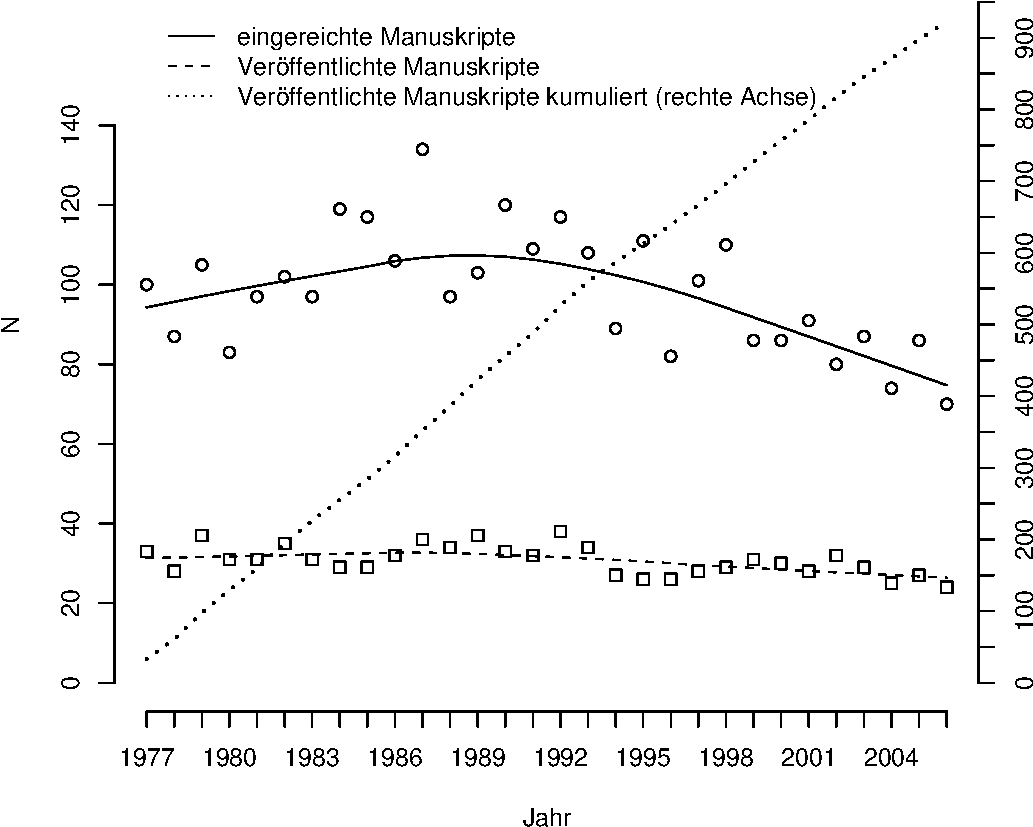
\includegraphics[scale = 0.5]{figKZFSS}
  \end{center}
\end{frame}


\begin{frame}
  \frametitle{Wie lassen sich große Mengen an Forschungsbefunden aufbereiten?}
  %%
  \begin{enumerate}
  \item \textbf{Bibliographien} ("`Fischer, Sonja (Hg.), 2005: Schulmüdigkeit
    und Schulverweigerung. Eine annotierte Bibliografie für die Praxis. München:
    DJI"')
  \item \textbf{Narrative Reviews} ("`Blumel, Susan R., 1992: Explaining Marital
    Success and Failure. S. 1-114 in: Bahr, Stephan J. (Hg.), Family Research. A
    Sixty Year Review, 1930-1990. New York: Lexington Books."')
  \item \textbf{Systematische Reviews\,/\,Forschungssynthesen}
    \begin{itemize}
    \item Qualitative Ausrichtung
    \item Quantitative Ausrichtung (Meta-Analyse)
    \end{itemize}
  \end{enumerate}
\end{frame}


\begin{frame}
  \frametitle{Grenzen von Bibliographien und narrativen (qualitativen) Reviews}
  \begin{itemize}
  \item<+-> Publikationsauswahl ist häufig unsystematisch und intersubjektiv nicht nachvollziehbar (\emph{confirmation bias}).
  \item<+-> Kein/Unzureichender Umgang mit \emph{widersprüchlichen} Befunden.
  \item<+-> Kein/Unzureichender Umgang mit \emph{vielen} empirischen Befunden.
  \item<+-> Ausmaß der Variabilität der Befunde kann nicht bestimmt werden.
  \item<+-> Erklärungen der Variabilität der Befunde können nicht überprüft werden.
  \end{itemize}
\end{frame}



\section{Begriffliche und konzeptionelle Grundlagen}

\begin{frame}<+->\frametitle{Vielfalt an Begriffen}
  %%
  \begin{itemize}
  \item Systematischer Review\,/\,Systematischer Übersichtsartikel
    (\emph{Systematic review})
  \item (Quantitative) Forschungssynthese (\emph{(Quantitative) Research
      synthesis})
  \item Integrativer Review (\emph{Integrative review})
  \item Meta-Analyse, Metaanalyse (\emph{Meta-analysis})
  \end{itemize}
\end{frame}


\begin{frame}
  \frametitle{Systematischer Reviews und Meta-Analysen}
  \begin{block}{Systematic (literature) review}
    "`A review that strives to comprehensively identify, appraise, and
    synthesize all the relevant studies on a given topic. Systematic reviews are
    often used to test just a single hypothesis, or a series of related
    hypothesis."'
  \end{block}
  %%
  \begin{block}{Meta-analysis}
    "`A review that uses a specific statistical technique for synthesizing the
    results of several studies into a single quantitative estimate (i.e. a
    summary effect size)"' \citep[19]{petticrew_systematic_2006}.
  \end{block}
\end{frame}


\begin{frame}\frametitle{Begriff der Meta-Analyse nach Glass (1976) }
  %%
  \enquote{Meta-analysis refers to the analysis of analyses. I use it to refer to the
  statistical analysis of a large collection on analysis results from individual
  studies for the purpose of integrating the findings} \citep[3]{glass_primary_1976}.
\end{frame}


\begin{frame}\frametitle{Begriff der Meta-Analyse nach Drinkmann (1990)}
  %%
  \enquote{Mit Meta-Analyse wird eine an den Kriterien empirischer Forschung
    orientierte Methode zur quantitativen Integration der Ergebnisse empirischer
    Untersuchungen sowie zur Analyse der Variabilität dieser Ergebnisse
    bezeichnet} \citep{drinkmann_methodenkritische_1990}.
\end{frame}


\begin{frame}
  \frametitle{Begriff der Meta-Analyse nach Borenstein et al (2009)}
  "`Meta-analysis refers to the statistical synthesis of results from a series
  of studies. While the statistical procedures used in a meta-analysis can be
  applied to any set of data, the synthesis will be meaningful only if the
  studies have been collected systematically. This could be in the context of a
  systematic review, the process of systematically locating, appraising, and
  then synthesizing data from a larger number of sources."' (Borenstein et
  al. 2009: xxif.)
\end{frame}


\begin{frame}\frametitle{Zum Verhältnis von systematischem Review, Forschungssynthese und Meta-Analyse: Ein Fazit}
  %%
  \begin{itemize}[<+->]
  \item Der Begriff (quantitative) Forschungssynthese (oder: quantitativer
    systematischer Review) beschreibt den gesamten
    Forschungsprozess. Forschungssynthesen haben sowohl \emph{qualitative} als
    auch \emph{quantitative} Elemente.
  \item Der quantitative (statistische) Teil einer Forschungssynthese heißt
    \emph{Meta-Analyse}.
  \end{itemize}
\end{frame}


\begin{frame}\frametitle{Systematik von Meta-Analysen I}
  %%
  \begin{itemize}[<+->]
  \item (Typ I: Qualitative Zusammenfassung, klassisches narratives Review)
  \item Typ II: Quantitative Zusammenfassung von publizierten, aggregierten
    Statistiken ("`publikationsbasierte"' Meta-Analyse)
  \item Typ III: Neuauswertung auf der Basis von zusammengeführten Originaldaten
    ("`originaldatenbasierte"' Meta-Analyse)
  \item Typ IV: Prospektiv geplante, gepoolte Auswertungen
  \end{itemize}
  
\citetext{Quellen: \citealt[149]{blettner_vergleich_1997}, \citealt[91]{finney_statistician_1995}}
\end{frame}


\begin{frame}\frametitle{Systematik von Meta-Analysen II}
  \begin{itemize}[<+->]
  \item Analyseebene: Aggregat- (APD) oder Individualdaten (IPD)
  \item Skalierung der abhängigen Variablen
  \item Forschungsdesign:
    \begin{itemize}
    \item Experiment oder Beobachtung\,/\,Befragung
    \item Intervention oder Zusammenhang
    \end{itemize}

  \end{itemize}
  (Sauerbrei und Blettner 2003)
\end{frame}



\begin{frame}
  \frametitle{Vier prototypische Forschungsprobleme von Forschungssynthesen}
  \begin{itemize*}
  \item<+-> Deskription
    \begin{itemize}
    \item<+-> Verbreitung des Schulschwänzens (Weiß 2008)
    \item<+-> Meta-Analyse von Studien zur Motivation von Stadt-Umland-Wanderung (Bleck/Wagner 2006)
    \end{itemize}
  \item<+-> Exploration: Meta-Analysen zum Stand der Ehescheidungsforschung (Wagner/Weiß 2003; 2004)
  \item<+-> Hypothesentests: Meta-Analysen zum Ehescheidungsrisiko in Europa (Wagner/Weiß 2006)
  \item<+-> Evaluation (von Interventionen): Meta-Analyse zur Wirksamkeit von Psychotherapien (Smith/Glass 1977)
  \end{itemize*}
\end{frame}



\begin{frame}
  \frametitle{Geschichte der Meta-Analyse}
  \begin{itemize}
  \item<+-> Erste Entwicklungen von Pearson (1904), Fisher (1932), Cochrane (1937).
  \item<+-> Zwischen 1930 und 1970 erfolgte keine Weiterentwicklung.
  \item<+-> Mitte der 1970er Jahre neues Forschungsinteresse: Glass (1976) prägt den Begriff "`Meta-Analyse"'
  \item<+-> In den 1980er Jahren bereits fünf Monographien: Glass et al. 1981, Hunter et al. 1982, Rosenthal
    1984, Light/Pillemer 1984, Hedges/Olkin 1985.
  \item<+-> Ab Mitte der 1980er Jahre kontinuierliche Anwendung und
    Weiterentwicklung der Methode in der Psychologie, Pädagogik und Medizin.
  \item<+-> In einigen Fächern bereits voller Institutionalisierungsgrad.
  \end{itemize}
\end{frame}


\begin{frame}\frametitle{Verschiedene Disziplinen kennen verschiedene "`Meta-Analyse-Schulen"'}
  %%
  \begin{itemize}
  \item Psychologie
  \item Erziehungswissenschaften
  \item Medizin, Gesundheitswissenschaften, Epidemiologie
  \item VWL (und BWL)
  \item (Soziologie)
  \end{itemize}
\end{frame}

\begin{frame}[plain]
  \frametitle{Soziologische Forschungssynthesen (SSCI)}
  \begin{center}
    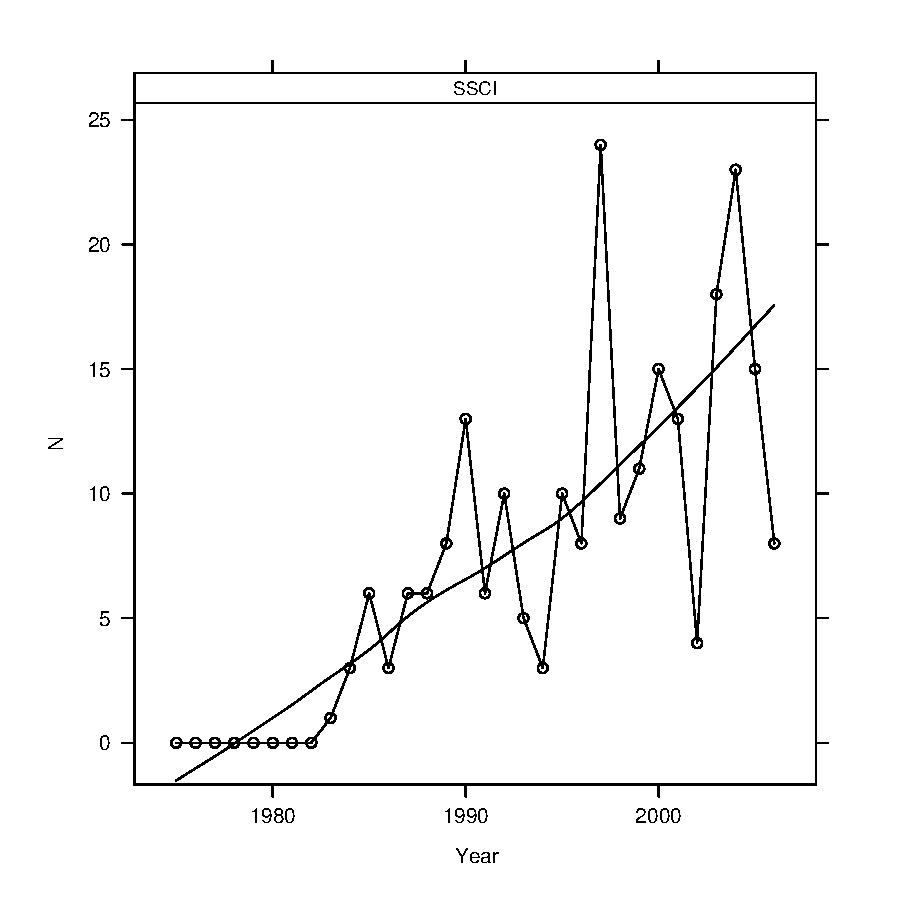
\includegraphics[scale = 0.55]{figLitDB-SSCI}
  \end{center}
\end{frame}





\section{Vorteile von Forschungssynthesen}


\begin{frame}
  \frametitle{Vorteile von (quantitativen) Forschungssynthesen}
  \framesubtitle{Systematisch, strukturiert und objektiv}
  %%
  Systematischer, strukturierter und objektiver (intersubjektiv nachvollziehbarer) Forschungsprozess:
  \begin{itemize}
  \item Dokumentation aller Arbeitsschritte (wie Literaturrecherche,
    Dateneingabe etc.)
  \item Offenlegung aller Regeln und abgeleiteten Entscheidungen
    bzgl. relevanter oder irrelevanter Forschungsbefunde
  \end{itemize}
\end{frame}


\begin{frame}
  \frametitle{Vorteile von (quantitativen) Forschungssynthesen}
  \framesubtitle{Differenzierte und aussagekräftige Ergebnisdarstellung}
  Forschungssynthesen erlauben eine differenziertere und aussagekräftigere
  Darstellung der Ergebnisse als narrative Reviews.
  \begin{itemize}
  \item Ein umfangreicher Forschungsstand kann auf wenige, klar zu
    interpretierende Statistiken reduziert werden.
  \item Quantifizierung der Ergebnisse geht aber \emph{nicht} mit einem
    Ausblenden von Unterschiedlichkeit/Heterogenität einher.
  \item Befunde einzelner, kleiner Studien können statistisch unbedeutsam sein
    (niedrige stat. \emph{power}); erst eine Forschungssynthese kann Nachweis
    statistischer Bedeutsamkeit liefern.
  \end{itemize}
\end{frame}



\begin{frame}
  \frametitle{Vorteile von (quantitativen) Forschungssynthesen}
  \framesubtitle{Erklärungen für einen heterogenen Forschungsstand}
 \begin{itemize}
 \item Systematische Kodierung von Studienbefunden und Studiencharakteristika.
 \item Dies ermöglicht die Untersuchung eines Zusammenhangs von Studienbefunden
   und Studiencharakteristika.
   \begin{itemize}
   \item<+-> Unterschiede werden \emph{entdeckt} und \emph{erklärt}.
   \end{itemize}
 \end{itemize}
\end{frame}






\section{Kritik an Forschungssynthesen und Meta-Analysen}

\begin{frame}
  \frametitle{Typische Kritik an Forschungssynthesen und Meta-Analysen}
  \begin{itemize}[<+->]
  \item "`Apples and Oranges"'
  \item "`Garbage in and Garbage out"'
  \item Unvollständiges Datenmaterial
  \item Verzerrungen durch selektives Publizieren (\emph{publication bias})
  \item Bivariate und multivariate Effektstärken
  \end{itemize}
\end{frame}

\begin{frame}\frametitle{Probleme von Meta-Analysen in der Soziologie}
  \begin{itemize}[<+->]
    \item APD Meta-Analysen: Fehlende Werte
    \item Integration von Regressionskoeffizienten
    \item Umgang mit abhängigen Effektstärken
  \end{itemize}
\end{frame}






 % Local variables:
 % TeX-open-quote: "\"`"
 % TeX-close-quote: "\"'"
 % End:



\part{Forschungssynthese als sozialwissenschaftliche Methode}\label{part:forsch-als-sozi}
\frame{\partpage}

\frame{\frametitle{Forschungssynthese als sozialwissenschaftliche Methode}
  \tableofcontents[part=3, hideallsubsections]}


\section{Der sozialwissenschaftliche Forschungsprozess}

\begin{frame}\frametitle{Relevante Dimensionen des Forschungsdesigns}
  \begin{itemize*}
  \item Wahl der Untersuchungseinheiten (bspw. Individuen vs. Kollektive)
  \item \textbf{Untersuchungsarten}
    \begin{itemize}
    \item Primäranalyse
    \item Sekundäranalyse
    \item Meta-Analyse
    \end{itemize}
  \item Zeitdimension (Querschnitt vs. Längsschnitt)
  \end{itemize*}
\end{frame}


\begin{frame}
  \frametitle{Untersuchungsarten}
  \begin{itemize*}
  \item<+-> \textbf{Primäranalyse}: Erstmalige Nutzung und Auswertung \emph{eines} Datensatzes.
  \item<+-> \textbf{Sekundäranalyse}: Erneute Nutzung \emph{eines} Datensatzes unter geänderten Bedingungen der
    Forschungsmethodik und\,/\,oder des theoretischen Bezugssystems.
  \item<+-> \textbf{Meta-Analyse}: Nutzung und Auswertung \emph{mehrerer} Datensätze\,/\,Studien mit gemeinsamer
    Fragestellung (womit noch \emph{nichts} über die Analyseeinheit gesagt wird!).
  \end{itemize*}
\end{frame}


\begin{frame}
  \frametitle{Elemente einer quantitativen Forschungssynthese}
  \begin{small}
    \begin{columns}[t]
    %%
      \begin{column}{0.35\linewidth}
        Diekmann (1997)
        \begin{enumerate}
        \item Formulierung und Präzisierung des Forschungsproblems
        \item Planung und Vorbereitung der Erhebung
        \item Datenerhebung
        \item Daten\-auswertung
        \item Berichterstattung
        \end{enumerate}
      \end{column}
      %%
      \begin{column}{0.3\linewidth}
        Cooper (1982)
        \begin{enumerate}
        \item Problem Formulation
        \item Data Collection
        \item Data Evaluation
        \item Analysis and Interpretation
        \item Public Presentation
        \end{enumerate}
      \end{column}
      %%
      \begin{column}{0.34\linewidth}
        Wagner\,/\,Weiß (2003)
        \begin{enumerate}
        \item Problem\,/\,\\Forschungsfrage
        \item Literatur-\- oder Datensatz\-recherche\- (allg. Datenerhebung)
        \item Dateneingabe
        \item Datenanalyse (Meta-Analyse)
        \item Ergebnis\-präsentation
        \end{enumerate}
      \end{column}
      %%
    \end{columns}
  \end{small}
\end{frame}



\section{Forschungsfrage}

\begin{frame}
  \frametitle{Bedeutung der Forschungsfrage}
  %%
  \begin{itemize}[<+->]
  \item Die Forschungsfrage \emph{muss} die interessierenden Merkmale und Zusammenhänge präzise beschreiben, um (später)
    relevante und irrelevante Studien/Publikationen voneinander unterscheiden zu können.
  \item Aus der Forschungsfrage lassen/sollten sich Kriterien für die Wahl relevanter bzw. irrelevanter Studien ableiten.
  \end{itemize}
\end{frame}


\begin{frame}
  \frametitle{Kriterien für eine gelungene Forschungsfrage}
  \begin{itemize}[<+->]
  \item Interessierende Variablen/Merkmale wurden klar definiert ("`Konzeptspezifikation"').
  \item Relevantes Forschungsdesign spezifizieren.
  \item Die Forschungsfrage in einen historischen, geographischen, theoretischen, methodologischen Kontext einbetten.
  \end{itemize}
\end{frame}


\begin{frame}[plain]
  \frametitle{Beispiel für Fragestellung (Wagner/Weiß 2006)}
  %%
  \begin{small}
    "`The aim of this paper is to summarize \alert{European} research on various \alert{divorce risks}. More precisely,
    we will examine how much divorce risks vary between European countries and whether such variations can be explained by
    country-specific macro-level factors. Are there any meaningful differences in the divorce risks between European
    countries?"'
  \end{small}
\end{frame}


\begin{frame}
  \frametitle{Beispiel für Fragestellung (Weiß 2008)}
  %%
  \begin{enumerate}[<+->]
  \item Wie viele Jugendliche schwänzen insgesamt die Schule?
  \item Wie hoch ist das Schulschwänzrisiko bei Jugendlichen mit Migrationshintergrund?
  \item Unterscheidet sich das Schulschwänzrisiko bei Jugendlichen mit Migrationshintergrund an Hauptschulen von den
    übrigen Schulformen?
  \end{enumerate}
\end{frame}


    \begin{frame}
      \frametitle{Beispiel für Fragestellung  (Wilson et al. 2008)}
      %%
      "`Objectives: To synthesize the extant empirical evidence on the effects of
      boot-camps and boot camp like programs on the criminal behavior (e.g., postrelease arrest, conviction, or
      reinstitutionalization) of convicted adult and juvenile offenders."'
    \end{frame}




\section{Datenerhebung: Literatur- und Studienrecherche}

\begin{frame}
  \frametitle{Ziel der (Literatur-)Recherche}
  %%
  Die Literaturrecherche entspricht der Phase der Datenerhebung im Rahmen einer Primäruntersuchung.
  \begin{itemize}[<+->]
  \item Erfassung eines möglichst großen Teiles der vorhandenen Literatur (Vollerhebung).
  \item Vermeidung von Verzerrungen:
    \begin{quotation}
      "`The point is not to track down every paper that is somehow related to
      the topic. (\ldots) The point is to avoid missing a useful paper that lies
      outside one's regular purview"' \citep[44]{white_scientific_1994}.
    \end{quotation}
  \item Systematische und transparente Suche.
  \end{itemize}
\end{frame}



\begin{frame}
  \frametitle{Spezifizierung des Untersuchungsgegenstandes der Forschungssynthese}
  \begin{itemize}[<+->]
  \item Abgrenzung zu anderen, verwandten Themen
  \item Definition der Grundgesamtheit
  \item Wichtige Untersuchungsvariablen
  \item Methodische Anforderungen
  \item Kulturelle und sprachliche Grenzziehungen
  \item \ldots
  \end{itemize}
\end{frame}



\subsection{Recherchestrategien}


\begin{frame}[plain]\frametitle{Genauigkeit und Vollständigkeit}
  \begin{center}
    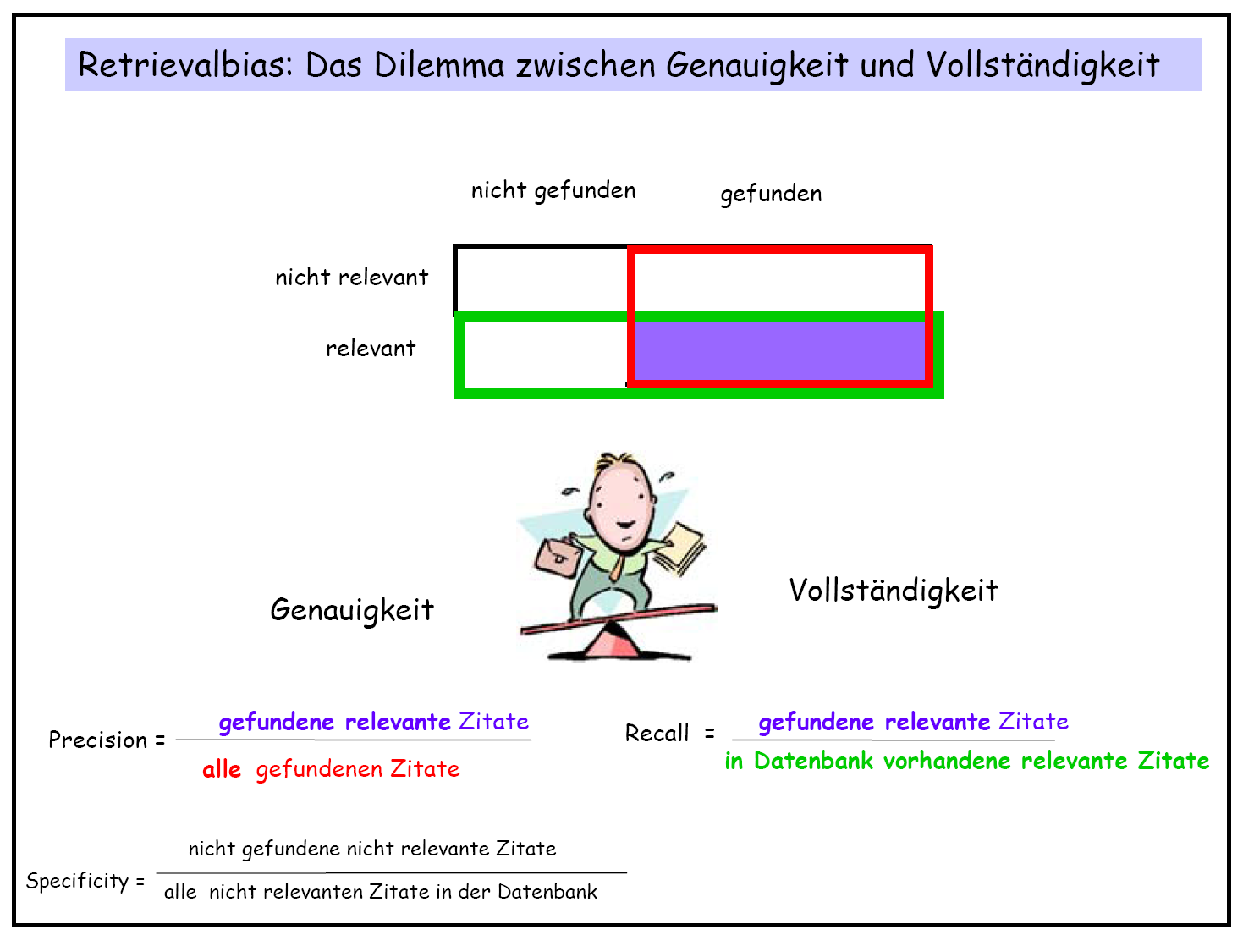
\includegraphics[scale=0.4]{figRecallPrecision}
  \end{center}
  \footnotesize{(Quelle: Motschall 2004: Medline-Suche mit PubMed,
    \url{http://www.agmb.de/04_mannheim/motschall.pdf})}
\end{frame}


\begin{frame}
  \frametitle{Ein unlösbares Problem}
  %%
  \begin{enumerate}[<+->]
  \item \emph{Recall} (Vollständigkeit): Anteil an gefundener relevanter
    Literatur im Verhältnis zur Gesamtzahl (hypothetische Größe) an
    \emph{relevanter} Literatur.
  \item \emph{Präzision} (Präzision, Genauigkeit): Anteil an gefundener
    relevanter Literatur im Verhältnis zur Anzahl \emph{insgesamt gefundener}
    (relevanter und nichtrelevanter) Literatur.
  \item Beide Maße stehen in einer inversen Beziehung und können nicht
    gleichzeitig optimiert werden:
    \begin{itemize}
    \item Je unspezifischer die Suche, desto höher der Recall und desto höher
      der Anteil an irrelevanten Publikationen $\Rightarrow$ hoher Arbeitsaufwand.
    \item Je spezifischer die Suche, desto höher die Precision und desto höher
      die Wahrscheinlichkeit, relevante Untersuchungen zu übersehen
      $\Rightarrow$ Repräsentativität der Stichprobe gefährdet.
    \end{itemize}
  \end{enumerate}
\end{frame}




\begin{frame}
  \frametitle{Suche in Literaturverweisen  ("`footnote chasing"')}
  %%
  \begin{block}{Vorgehen}
    \begin{itemize}[<+->]
    \item Reviews
    \item thematisch verwandte Artikel, Bücher oder Zeitschriften
    \item Bibliographien
    \end{itemize}
  \end{block}
  \pause
  \begin{block}{Beurteilung}
    \begin{itemize}[<+->]
    \item[$+$] guter Einstieg in die Suche
    \item[$+$] meist relativ hohe Präzision
    \item[$-$] selektive, persönliche Auswahl (eigene Untersuchungen / Literaturverweise) $\rightarrow$ Verzerrungen
    \item[$-$] Aktualität der Literatur hängt von Referenzquelle ab. 
    \end{itemize}
  \end{block}
\end{frame}


\begin{frame}
  \frametitle{Suche in (Fach-)Datenbanken: Vorgehen}
  %%
  \begin{itemize}[<+->]
  \item z.B. Wiso 3, SOLIS/FORIS, Sociological Abstracts, SocioFile etc.
  \item  Fachdatenbanken umfassen:
    \begin{itemize}
    \item  meist nur publizierte Artikel
    \item ab einem bestimmten Jahr
    \item innerhalb bestimmter geographischer Grenzen $\rightarrow$ deswegen: Charakteristika der Datenbanken beachten
    \end{itemize}
  \item Übereinstimmung von Suchabfrage mit den Angaben in der Datenbank notwendig $\rightarrow$ richtige Benutzung
    Boolscher Operationen, vorsichtiger Umgang mit Begriffen
  \end{itemize}
\end{frame}


\begin{frame}
  \frametitle{Suche in (Fach-)Datenbanken: Beurteilung}
  %%
  \begin{itemize}[<+->]
  \item[$+$] Vermeidet Verzerrungen aufgrund persönlicher Auswahl.
  \item[$-$] Relativ niedrige Präzision, sofern die Recall-Rate akzeptabel sein soll.
  \item[$-$] Verzerrungen aufgrund der in die Datenbanken aufgenommenen Artikel.
  \end{itemize}
\end{frame}

\begin{frame}
  \frametitle{Suche in Zitationsdatenbanken}
  %%
  \begin{block}{Vorgehen}
    z.B. Social Science Citation Index
  \end{block}
  \pause
  \begin{block}{Beurteilung}
    \begin{itemize}
    \item[$+$] ermöglicht das Auffinden von Literatur aus unterschiedlichen Fachbereichen
    \item[$+$] umfasst neueste Publikationen
    \item[$+$] relativ hohe Recall-Rate
    \item[$-$] Verzerrungen aufgrund der in die Datenbanken aufgenommenen Artikel
    \end{itemize}
  \end{block}
\end{frame}

\begin{frame}
  \frametitle{Kommunikation mit den peers}
  %%
  \begin{block}{Vorgehen}
    \begin{itemize}
    \item Konferenzen
    \item Anfragen bei Forschern
    \item Anfragen bei staatlichen Einrichtungen
    \end{itemize}
  \end{block}
  \begin{block}{Beurteilung}
    \begin{itemize}
    \item[$+$] ermöglicht Auffinden nicht publizierter Literatur
    \item[$+$] sehr hohe Präzision
    \item[$-$] selektive Auswahl $\rightarrow$ Verzerrungen
    \end{itemize}
  \end{block}
\end{frame}


\begin{frame}\frametitle{Systematische Suche in Bibliotheken und Zeitschriften (Browsing)}

  \begin{block}{Vorgehen}
    \begin{itemize}
    \item Systematisches Durchsuchen von Zeitschriftenjahrgängen (bspw. letzte 10 Jahrgänge von JMF)
    \end{itemize}
  \end{block}
  %%
  \begin{block}{Beurteilung}
    \begin{itemize}
    \item[$-$] meist geringe Präzision, zeitaufwendig
    \item[$+$] thematisch eng gefasste Zeitschriften oder Bibliotheksbereiche können aber die Suche sinnvoll ergänzen
    \end{itemize}
  \end{block}
\end{frame}




\subsection{Bewertung und Auswahlkriterien}


\begin{frame}
  \frametitle{Auswahlkriterien}
  %%%
  \begin{small}
    Die Auswahlkriterien definieren die Grundgesamtheit und betreffen die Generalisierbarkeit der Ergebnisse der
    Forschungssynthese. Relevante Dimensionen sind u.a.:
    \begin{itemize}[<+->]
    \item Forschungsdesign (Längsschnitt/Querschnitt, Experiment/Umfrage/\ldots)
    \item Messung zentraler Konstrukte
    \item Grundgesamtheit der einzelnen Studie (Stichprobenzusammensetzung, Alter, Ost/West, \ldots)
    \item Zeitlicher und geographischer Kontext der Studie (Jahr der Stichprobenerhebung, Publikationsjahr, \ldots)
    \item Qualität der Studien (inkl. ausreichend Daten für Durchführung stat. Analysen)
    \item Publikationstyp (un-/veröffentlichte Literatur, graue Literatur, \ldots)
    \item \ldots
    \end{itemize}
  \end{small}
\end{frame}


\begin{frame}
  \frametitle{Beispiel für Auswahlkriterien (Wagner/Weiß 2006)}
  %%
  \begin{small}
    "`Publications dealing with our research question should meet the following
    criteria to be included in our meta-analysis: on the one hand, we were
    interested in publications in which marital stability is the dependent
    variable.  On the other hand, we limited our search to publications that
    explicitly used European longitudinal data sets. The countries considered
    here are the 18 countries of the European Economic Area (EEA), the candidate
    countries for the European Union, and Switzerland"' (Wagner/Weiß 2006: 487).
  \end{small}
\end{frame}


\begin{frame}
  \frametitle{Beispiel für Auswahlkriterien (Weiß 2008)}
  "`Letztlich orientierte sich die Auswahl geeigneter Datensätze an drei
  Kriterien: (1) Der Datensatz enthält Angaben zur selbst- oder fremdberichteten
  unentschuldigten Schulabwesenheit. Dabei ist gleichgültig, für welchen
  Zeitraum das Schulschwänzen erfasst oder wie präzise die Häufigkeit des
  Phänomens gemessen wurde. (2) Die Datensätze sind für Sekundäranalysen
  verfügbar. (3) Die Stichprobe wurde in Deutschland gezogen, ohne jedoch
  vorauszusetzen, nur Schüler mit deutscher Staatsangehörigkeit zu erfassen"'
  (Weiß 2008).
    \end{frame}


    \begin{frame}
      \frametitle{Beispiel für Auswahlkriterien (Wilson et al. 2008)}
      "`Selection Criteria: The eligibility criteria were (a) that the study
      evaluated a correctional boot camp, shock incarceration, or intensive
      incarceration program; (b) that the study included a comparison group that
      received either probation or incarceration in an alternative facility; (c)
      that the study participants were exclusively under the supervision of the
      criminal or juvenile justice system; and (d) that the study reported a
      post-program measure of criminal behavior, such as arrest or conviction"'
      (Wilson et al. 2008: 2).
    \end{frame}




\subsection{Dokumentation der Recherche und Verwaltung der Quellen}

\begin{frame}
  \frametitle{Verwaltung der Literatur}
  \begin{itemize}[<+->]
  \item Tabellenkalkulation (OO-Calc, MS-Excel).
  \item (Kostenpflichtige) Programmee zur Literaturverwaltung wie Endnote,
    Reference Manager etc.
  \item (Kostenfreie) Programme wie Mendeley, Zotero oder RevMan.
  \end{itemize}
  \emph{Ein} Argument für die Verwendung eines bestimmten Programms ist eine
  offene Schnittstelle auf die bspw. Statistiksoftware zugreifen kann (bieten
  etwa Mendeley oder Zotero).
\end{frame}


\begin{frame}[plain]
  \frametitle{Dokumentation der Literaturrecherche (Weiß 2008)}
  \begin{center}
    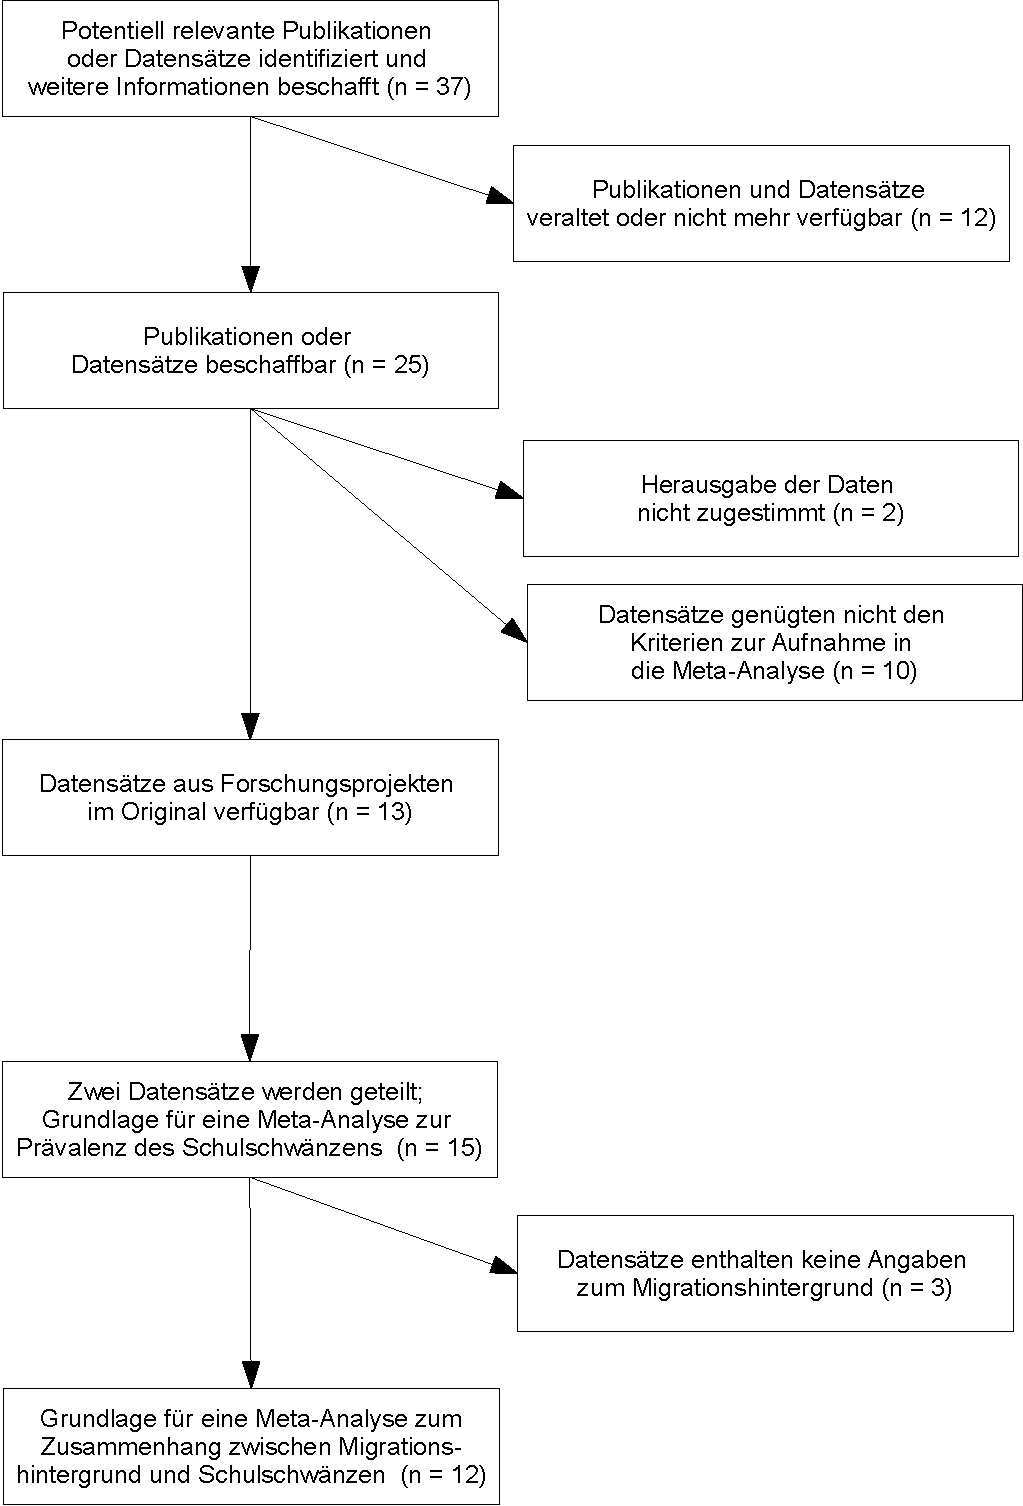
\includegraphics[width = 0.5\textwidth]{figRechercheDatensaetze}
  \end{center}
\end{frame}


\begin{frame}[plain]
  \frametitle{Dokumentation der Literaturrecherche \citep{lorant_socioeconomic_2003}}
  \begin{center}
    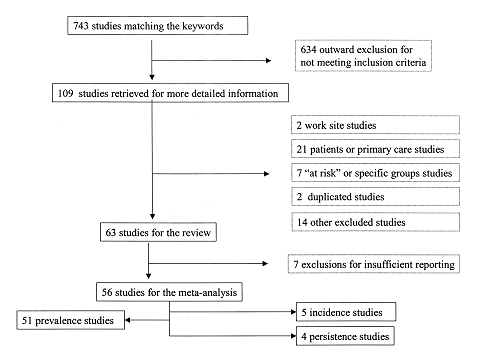
\includegraphics[width=0.85\textwidth]{figDokRechercheLorant}  
  \end{center}
\end{frame}


\subsection{Stichprobenselektivität}

\begin{frame}
  \frametitle{Quellen der Verzerrungen bei der Literatursuche}
  %%
  \begin{itemize}[<+->]
  \item Subjektive Auswahl bei Reviews (ebenfalls eher statistisch signifikante Ergebnisse)
  \item Verzerrung durch Sprachbarrieren
  \item Verzerrung durch einseitige Literaturrecherche
  \item \ldots
  \item $\rightarrow$ Verzerrungen führen tendenziell zu einer Überschätzung der Effektstärken.
  \end{itemize}

  Weitere Informationen zum Thema "`Publication Bias"' finden sich ab Folie \pageref{sec:pubbias}.

\end{frame}

\section{Datenvercodung/-eingabe und Effektstärken}


\begin{frame}
  \frametitle{Übersicht}
  \begin{itemize}[<+->]
  \item Nach der Identifikation relevanter Publikationen müssen die darin enthaltenen Informationen erfasst werden
    (ähnelt einer Inhaltsanalyse).
  \item Festlegen, welche Informationen für die Fragestellung wichtig sind.
  \item Fragebogen (Codierbogen) erstellen.
  \item Insbesondere auf die Vergleichbarkeit der empirischen Befunde achten.
  \end{itemize}
\end{frame}



\begin{frame}
  \frametitle{Datenerhebung und -vercodung}
  \begin{itemize}[<+->]
  \item Welche Informationen aus den Studien besitzen Relevanz (Synthese\,/\,Heterogenität)?
    \begin{itemize}
    \item Publikationsbefunde (Statistiken, Effektstärken, \ldots)
    \item Publikationsmerkmale (Publikationstyp, Publikationsjahr, \ldots)
    \item Studien-/Stichprobenmerkmale (Erhebungsjahr, Organisation, Stichprobendesign, \ldots)
    \item Methode und Qualität (Statistische Verfahren, bestimmte Qualitätskriterien, \ldots)
    \end{itemize}
  \item Konstruktion eines \glq Fragebogens\grq\ (Codierbogen).
  \item Problem: Auswahl überflüssiger oder Auslassen bedeutsamer Variablen.
  \end{itemize}
\end{frame}


% \begin{frame}
%   \frametitle{Studienmerkmale XXX}

%   \begin{itemize}
%   \item Stichprobenquelle
%   \item Stichprobenmerkmale (demographische Angaben: sozioökonomische  Herkunft, Alter, Geschlecht etc.;
%     Personenmerkmale: kognitive Fähigkeiten, Charaktereigenschaften)
%   \item unabhängige Variablen
% 	allgemeine Beschreibung (kategorial oder metrisch etc.)
% 	Ausprägungen
% Methode
% 	Studiendesign

% Quellen der Meta-Analyse
% 	Art der Veröffentlichung (Zeitschrift, Buch, Dissertation etc.)
% 	Publikationsjahr
% 	Sprache in der veröffentlicht wurde
% 	finanzielle Unterstützung der Studie und durch wen
% 	Eigenschaften des Forschers (Geschlecht, Zugehörigkeit zu Institut XY etc.)
%   \end{itemize}
% \end{frame}


\begin{frame}
  \frametitle{Beispiel für Codierbogen (Auszug)}
  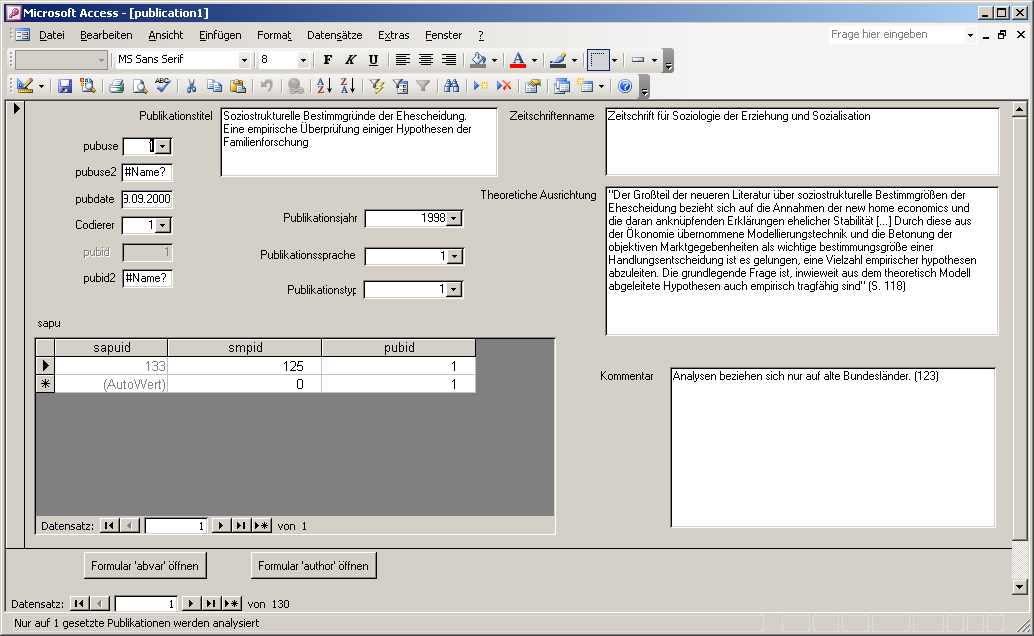
\includegraphics[scale = 0.3]{figCodierbogenScheidung}
\end{frame}


\begin{frame}
  \frametitle{Beispiel für Codierbogen  (Auszug)}
  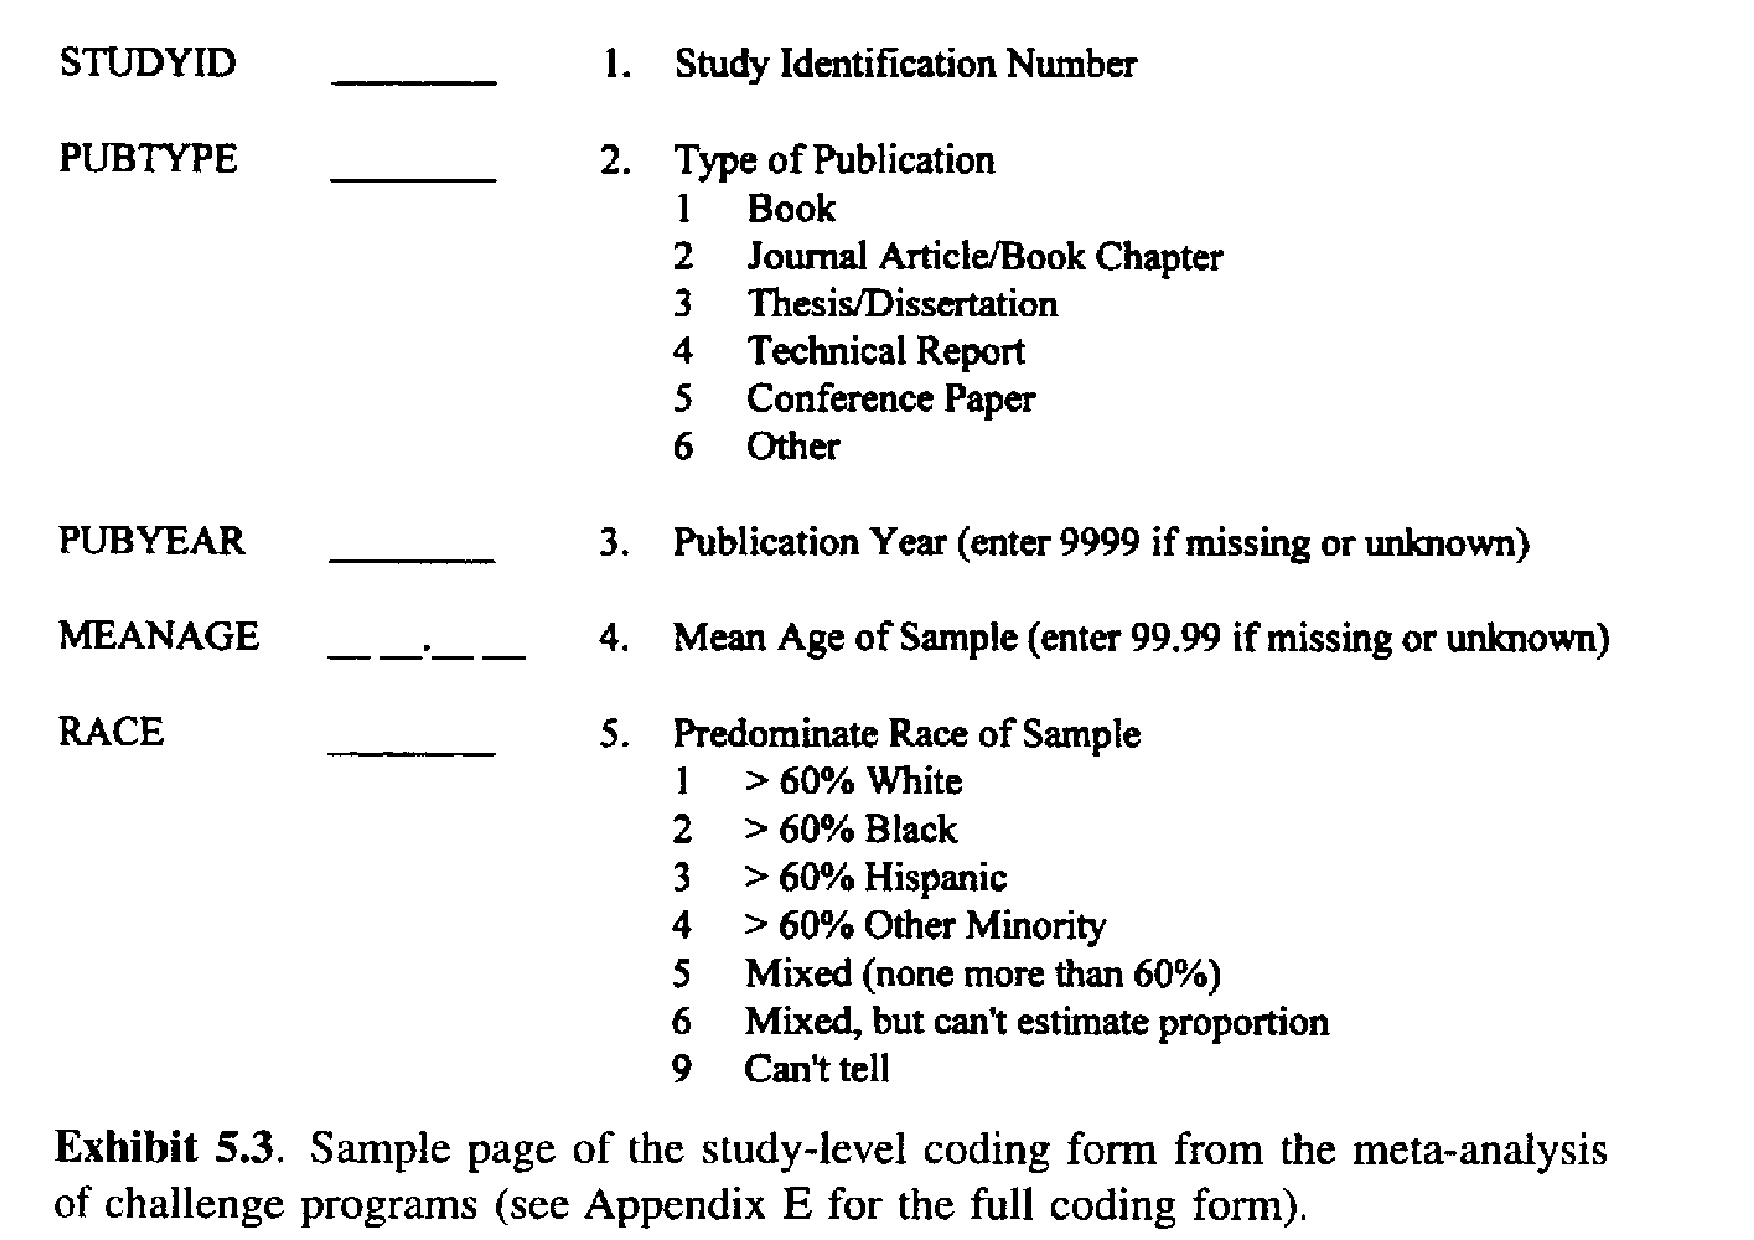
\includegraphics[scale = 0.3]{figKodierschema.pdf}
\end{frame}


\begin{frame}
  \frametitle{Was ist ein (empirischer) Forschungsbefund?}
  %%
  \begin{small}
    \begin{itemize}[<+->]
    \item Glass (1976: 6) weist die \emph{Effektstärke} als Mittelwertsdifferenz zwischen Experimental- und
      Kontrollgruppe aus, die durch Division mit der Gruppenvarianz (angenommen wird eine Gleichheit der
      Gruppenvarianzen) standardisiert wird.
    \item Nach Rosenthal (1991) beschreibt ein Forschungsbefund den Zusammenhang zwischen Variable $X$ und Variable
      $Y$. Dieser Zusammenhang enthält zwei Elemente:
      \begin{enumerate}
      \item ein Schätzer der Größe des Zusammenhangs (Effektstärke, engl. "`effect size"').
      \item eine Maßzahl für die Reliabilität der Effektgröße (Standardfehler, Konfidenzintervalle, $p$-Wert).
      \end{enumerate}
    \item Allgemein lässt sich ein Forschungsbefund definieren als "`[\ldots] statistical representation of one
      empirical relationship involving the variable(s) of interest to the meta-analysis measured on a single subject
      sample."'(Lipsey/Wilson 2000: 35)
    \end{itemize}
  \end{small}
\end{frame}



\begin{frame}
  \frametitle{Effektstärke}
  %%
  \begin{itemize*}
  \item Die wesentliche Eigenschaft einer Effektstärke ist nach Hedges\,/\,Olkin (1985: 7) ihre Skaleninvarianz
    (ermöglicht die Vergleichbarkeit zwischen Studien).
  \item Wünschenswerte Eigenschaften von Effektstärken sind zudem Informationen über \emph{Größe} und \emph{Richtung}
    des Zusammenhangs zwischen Variablen.
  \end{itemize*}
\end{frame}

\begin{frame}
  \frametitle{Von der Hypothese zur Effektstärke}
  %%
  \begin{itemize}[<+->]
  \item Unterschieds- oder Zusammenhangshypothesen
    \begin{itemize}
    \item Unterschiedshypothese: "`Wenn Jugendliche eine Klasse wiederholen müssen, dann steigt ihr Schwänzrisiko."'
    \item Zusammenhangshypothese: "`Je schlechter das Klassenklima vom einzelnen Schülern bewertet wird, desto höher
      auch das individuelle Schwänzrisiko."'
    \end{itemize}
  \item Gerichtete oder ungerichtete Hypothesen
    \begin{itemize}
    \item Unterschiedshypothesen (Wenn\ldots dann) und Zusammenhangshypothesen sind \emph{gerichtete} Hypothesen.
    \item Ungerichtete Hypothesen behaupten lediglich einen Unterschied, ohne jedoch eine Richtung (besser --
      schlechter, höher -- niedriger etc.) vorzugeben.
    \end{itemize}
\end{itemize}
\end{frame}


\begin{frame}
  \frametitle{Typen von Effektstärken\,/\,Forschungsbefunden (1)}
  %
  \begin{itemize}[<+->]
  \item Kontinuierliche Merkmale:
    \begin{itemize}
    \item Maßzahlen der $r$-Familie: z.B. $r$, ($\phi$), $r_{pb}$ und $\rho$
    \item Maßzahlen der $d$-Familie: z.B. Hedges' $g$, Glass' $\Delta$ und Cohen's $d$
    \end{itemize}
  \item Dichotome (kategoriale) Merkmale: z.B. odds ratio, risk ratio, $\phi$
  \item Teststatistiken (etwa $t$-, $F$- oder $\chi^2$-Werte)
  \item Narrative Darstellung signifikant positiver, negativer oder nichtsignifikanter Effekte
  \item $p$-Werte (kond. Wahrscheinlichkeit der fälschlichen Zurückweisung der $H_0$, gegeben, dass in GG die $H_0$
    gilt; $\alpha$-Fehlerwahrscheinlichkeit)
  \item \ldots
  \end{itemize}

  (mehr Informationen zu ES auf den Folien \pageref{sec:effectstaerken}ff verfügbar)

\end{frame}



\begin{frame}
  \frametitle{Typen von Effektstärken\,/\,Forschungsbefunden (2)}
  %%
  Effektstärken (besser: Forschungsbefunde) lassen sich aber auch nach der Anzahl der Variablen unterscheiden:
    \begin{itemize}
    \item Univariate Effektstärken (bspw. Anteile, Mittelwerte)
    \item Bivariate Effektstärken (bspw. $d$, $r$, odds ratio)
    \item Multivariate Effektstärken (bspw. Regressionskoeffizienten)
    \end{itemize}
  \end{frame}



\begin{frame}
  \frametitle{Welche meta-analytischen Verfahren gibt es für die verschiedenen Formen von Forschungsbefunden?}
  \begin{enumerate}
  \item Vote counting
  \item Zusammenfassen von Signifikanzwerten
  \item Zusammenfassen von Effektstärken (Effektstärkensynthese)
  \item Zusammenfassen von Korrelationsmatrizen
  \item \ldots
  \end{enumerate}
\end{frame}


\begin{frame}
  \frametitle{Ein Vorgriff auf das Berechnen einer mittleren Effektstärke}
  \begin{itemize}[<+->]
  \item Auf Grundlage der Ergebnisse ($T_j$) von $k$ unabhängigen Studien wird
    im einfachsten Fall eine mittlere Effektstärke ($\overline{T}$) als
    gewichtetes arithmetisches Mittel berechnet:
    \begin{equation*}
      \overline{T} = \frac{\sum\limits^k_{j=1}{w_j \times T_j}}{\sum\limits^k_{j=1}{w_j}}
    \end{equation*}

  \item Neben den ES werden auch noch \alert<+->{Gewichte} benötigt:
    \begin{itemize}
    \item Fallzahl ($w_j = n_j$)
    \item Inverse quadrierte Standardfehler (Fehlervarianz): $w_j = \frac{1}{SE_j^2}$
    \end{itemize}
  \end{itemize}
\end{frame}


\begin{frame}[plain]
  \frametitle{Abhängige Effektstärken}\label{slide:abhaeng-es}
  
  \begin{footnotesize}
    Wie entstehen abhängige Effektstärken?
    \begin{itemize}
    \item Multiple Befundstatistiken pro Person (bspw. mehrere Testergebnisse; hierarchische Regressionsmodelle).
    \item Verschiedene Treatment-Gruppen haben eine gemeinsame Kontrollgruppe.
    \item \ldots
    \end{itemize}

    Umgang mit abhängigen ES:
    \begin{itemize}
    \item Die "`beste"' (oder "`mittlere"') ES wählen.
    \item Zunächst pro Set abh. ES eine Meta-Analyse durchführen (Stufe 1) und
      dann eine zweite Meta-Analyse über die gemittelten ES durchführen (Stufe
      2).
    \item Bei multiplen ES (mehrere abh. Variablen) pro Personen pro Gruppe eine
      Meta-Analyse durchführen.
    \item Multivariate Meta-Analyse (Korrelationsmatrix muss vorliegen)
    \item Mehrebenen-Meta-Analyse
    \end{itemize}

    \citep[Quellen: ][]{kim_degree_2010, lambert_meta-analysis_1996,
      raudenbush_modeling_1988, thompson_impact_2013}
  \end{footnotesize}
\end{frame}



\section{Effektstärken (ES)}\label{sec:effectstaerken}

\begin{frame}\frametitle{Effektstärkenschätzer und -parameter}

  Bezüglich des Umgangs mit Effektstärken im Rahmen einer Meta-Analyse ist die
  folgende Unterscheidung wichtig:
  \begin{itemize}
  \item (Effektstärken-)\emph{Schätzer} werden in den Publikationen berichtet
    und basieren auf einer \emph{bestimmten} Stichprobe (\emph{sample effect
      sizes}).
  \item (Effektstärken-)\emph{Parameter} repräsentieren den \emph{wahren} Wert
    in der Grundgesamtheit (\emph{population (or true) effect size}).
  \end{itemize}

  Ein Ziel von Meta-Analyse ist, mit Hilfe der Effektstärken\emph{schätzer}
  den Populationsparameter zu schätzen. Neben dem eigentlichen ES-Schätzer wird
  (fast) immer auch der \emph{Standardfehler} als Gewicht benötigt.
   (Campbell Collaboration 2009: 5).
\end{frame}


\begin{frame}\frametitle{Übersicht und weiterführende Informationen}
  \begin{itemize}
  \item Hier werden
    \begin{itemize}
    \item die Produkt-Moment-Korrelation $r$,
    \item Cohens $d$,
    \item Hedges $g$,
    \item das Odds Ratio sowie
    \item der semi-partielle Korrelationskoeffizient (für Koeffizienten von
      multiplen linearen Regressionsmodellen) näher erläutert.
    \end{itemize}
  \item Gute Übersichten liefern u.a.
    \begin{itemize}
    \item \citet{borenstein_introduction_2009}, \citet{lipsey_practical_2001}
    \end{itemize}
  \end{itemize}
\end{frame}


\subsection{Effektstärken der $r$-Familie}


\begin{frame}
  \frametitle{Übersicht}
  %%
  \begin{itemize}[<+->]
  \item Produkt-Moment-Korrelation $r$ von (Bravais und) Pearson (beide Merkmale haben metrisches Skalenniveau)
  \item Korrelationskoeffizient nach Spearman (beide Merkmale haben ordinales Skalenniveau)
  \item Punkt-biserale Korrelation (ein Merkmal dichotom, ein Merkmal metrisch)
  \item \ldots
  \end{itemize}
  (Borenstein et al. 2009: 23ff)
\end{frame}


\begin{frame}[shrink = 5]
  \frametitle{Produkt-Moment-Korrelation}
  \framesubtitle{Eigenschaften der Effektstärke}
  %%
  \begin{itemize}[<+->]
  \item Pearsons $r$ errechnet sich aus der normierten Kovarianz und misst die Stärke des Zusammenhanges zweier Variablen.
  \item Der Korrelationskoeffizient liegt zwischen $-1$ (bei vollständig gegenläufigem Zusammenhang) und $+1$ (bei
    vollständig gleichläufigem Zusammenhang).
  \item Pearsons r ist ebenso wie die Kovarianz bei fehlendem Zusammenhang gleich 0.
  \item Der Korrelationskoeffizient kann nur für metrische Daten angewandt werden. Eine Ausnahme sind zwei dichotome
    Variablen, die 0/1 kodiert sind. In diesem Fall entspricht der Korrelationskoeffizient der Chi-Quadrat-basierten Maßzahl $\phi$.
  \end{itemize}
\end{frame}


\begin{frame}
  \frametitle{\large{Der Korrelationskoeffizient r von Bravais und Pearson}}
  \framesubtitle{Definition der Effektstärke}
  %%
  Pearsons $r$ lässt sich auch als die Kovarianz von $X$ und $Y$ ($S_{XY}$) dividiert durch das
  Produkt der Standardabweichungen von $X$ und $Y$ ($S_X$ und $S_Y$) definieren.
  % Durch die Normierung der Kovarianz fallen zum einen die Dimensionen der Ausgangsvariablen weg, zum anderen liegt der
  % Wertebereich des Koeffizienten immer zwischen $-1$ und +1. So können auch die unterschiedlichsten Verteilungen
  % miteinander verglichen werden.
  \begin{equation}
    r = \frac{S_{XY}}{S_X \cdot S_Y}
  \end{equation}
  mit:\\
  \begin{equation}
    S_{XY} = \frac{1}{n-1}\sum\limits^n_{i = 1}(x_i - \overline{x}) \cdot (y_i - \overline{y})
  \end{equation}

  \begin{equation}
    S_x = \sqrt{\frac{1}{n-1} \sum\limits^n_{i = 1} (x_i - \overline{x})^2} \text{  und  }
    S_y = \sqrt{\frac{1}{n-1} \sum\limits^n_{i = 1} (y_i - \overline{y})^2}
  \end{equation}
\end{frame}


\begin{frame}\frametitle{Die Fisher Z-Transformation}
  %%
  Bei der Befundsynthese von Korrelationskoeffizienten gilt es zu beachten, dass diese (i.A.) erst transformiert werden
  müssen. Diese Transformation hat zwei Gründe:
  \begin{enumerate}[<+->]
  \item Der Korrelationskoeffizient ist nicht normalverteilt.
  \item Der Standardfehler lässt sich nur für den transformierten Korrelationskoeffizienten bestimmen, da die
    Z-Transformation varianzstabilisierend ist und die Varianz von $z_r$ nicht von $r$ abhängt.
  \end{enumerate}
  \pause
  Es gilt dann:
  \begin{itemize}[<+->]
  \item Z-Transformation von $r$: $z_r=0.5 \cdot ln(\frac{1+r}{1-r})$.
  \item Standardfehler für $z_r$: $SE_{z_r}=\frac{1}{\sqrt{N-3}}$ mit $N$: Fallzahl.
  \item Rücktransformation $z_r$ zu $r$: $r=\frac{e^{2 \cdot z_r}-1}{e^{2 \cdot z_r}+1}$.
  \end{itemize}
\end{frame}


\begin{frame}\frametitle{Beispiel Fisher Z-Transformation}
  
  \begin{itemize}
  \item Gegeben sind: $r=0.13$ und $n=123$
  \item Fisher Z-transformierte Korrelation: $z_r = 0.5 \cdot
    \ln(\frac{1+0.13}{1-0.13})$ = 0.1307
  \item Standardfehler:
    $SE_{z_r}=\frac{1}{\sqrt{123-3}}$=0.0913
  \item Rücktransformation: $r=\frac{e^{2 \cdot 0.1307} -1}{e^{2 \cdot 0.1307} +
      1}$ = 0.13
  \end{itemize}
  
\end{frame}


\subsection{Effektstärken der $d$-Familie}

\begin{frame}
  \frametitle{Übersicht}
  %%
  \begin{itemize}[<+->]
  \item Die abhängige Variable ist metrisch skaliert, die unabhängige Variable
    ist ein (dichotomer) Faktor (Gruppenmerkmal, Pre-Post-Vergleich).
  \item Unstandardisierte Mittelwertdifferenz
    \begin{itemize}
    \item Für zwei unabhängige Gruppen
    \item Für abhängige Gruppen (etwa Pre-Post-Tests) (wird nicht weiter erläutert)
    \end{itemize}
  \item Standardisierte Mittelwertdifferenzen (Cohens $d$, Hedges $g$)
    \begin{itemize}
    \item Für zwei unabhängige Gruppen
    \item Für abhängige Gruppen (etwa Pre-Post-Tests) (wird nicht weiter erläutert)
    \end{itemize}
  \item \ldots
  \end{itemize}
  (Borenstein et al. 2009: 22ff)
\end{frame}


\begin{frame}\frametitle{Unstandardisierte Mittelwertdifferenz}

  Die unstandardisierte Mittelwertdifferenz zweier unabhängiger Mittelwerte
  $\mu_1$ und $\mu_2$ ist definiert als:

  \begin{equation}
    \Delta = \mu_1 - \mu_2,
  \end{equation}

  Die Schätzung von $\widehat{\Delta} = D$ erfolgt über zwei unabhängige
  Stichprobenmittelwerte $\overline{Y_1}$ und $\overline{Y_1}$:

  \begin{equation}
    D = \overline{Y_1} - \overline{Y_1}.
  \end{equation}
  
\end{frame}



\begin{frame}[plain, shrink]\frametitle{Varianz der unstandardisierten
    Mittelwertdifferenz}\label{sec:effektstarken-der-d}

  \begin{itemize}
  \item Seien $S_1$ und $S_2$ die beiden Standardabweichungen von $Y_1$ und
    $Y_2$ und angenommen, diese unterscheiden sich \emph{nicht} in der
    Population, dann ergibt sich die Varianz von $D$ als:
    
    \begin{equation}
      V_D = \frac{n_1 + n_2}{n_1n_2}S^2_{pooled} 
    \end{equation}
    
    mit
    
    \begin{equation}\label{eq:sd_pooled}
      S_{pooled} = \sqrt{\frac{(n_1-1)S^2_1 + (n_2-1)S^2_2}{n_1+n_2-2}}.
    \end{equation}
    
  \item Für unterschiedliche Populationsstandardabweichungen ergibt sich die Varianz
    von $D$ nach:
    
    \begin{equation}
      V_D = \frac{S^2_1}{n_1} + \frac{S^2_2}{n_2}.
    \end{equation}
  \end{itemize}
  
  Der Standardfehler von $D$ ergibt sich aber immer nach: 

  \begin{equation}
    SE_D = \sqrt{V_D}.
  \end{equation}
\end{frame}


\begin{frame}\frametitle{Beispiel unstandardisierte Mittelwertdifferenz}
  \begin{itemize}
  \item Gegeben sind:
    \begin{itemize}
    \item $\overline{Y}_1=103$, $S_1=5.5$, $n_1=50$
    \item $\overline{Y}_2=100$, $S_2=4.5$, $n_2=50$.
  \end{itemize}
  \item $D$ ist: $103-100=3$
  \item $SE_D$ ist (angenommen $\sigma_1 = \sigma_2$):
    \begin{itemize}
    \item $S_{pooled}=\sqrt{\frac{(50-1)5.5^2 + (50-1)4.5^2}{50+50-2}}=5.0249$
    \item $V_D = \frac{50+50}{50 \cdot 50} \cdot 5.0249 = 1.0100$
    \item $SE_D= \sqrt{1.0100} = 1.0050$
  \end{itemize}
  \end{itemize}
  \vfill
  \citep[22]{borenstein_introduction_2009}
\end{frame}



\begin{frame}\frametitle{Standardisierte Mittelwertdifferenz (Cohens $d$)}

  Die standardisierte Mittelwertdifferenz zweier unabhängiger Mittelwerte
  $\mu_1$ und $\mu_2$ ist definiert als:

   \begin{equation}
     \delta = \frac{\mu_1 - \mu_2}{\sigma}, \text{ wobei } \sigma_1 = \sigma_2 =\sigma,
   \end{equation}
   Die Schätzung von $\widehat{\delta} = d$ erfolgt über die zwei
   Stichprobenmittelwerte $\overline{Y_1}$ und $\overline{Y_1}$:
   \begin{equation}
     d = \frac{\overline{Y_1} - \overline{Y_1}}{S_{within}} \text{ (für $S_{within}$ siehe Gleichung \ref{eq:sd_pooled})}.
   \end{equation}
 
 \end{frame}

 
 \begin{frame}\frametitle{Varianz der standardisierten
     Mittelwertdifferenz}

   Seien $S_1$ und $S_2$ die beiden Standardabweichungen von $Y_1$ und $Y_2$ und
   angenommen, diese unterscheiden sich \emph{nicht} in der Population, dann
   ergibt sich die Varianz von $d$ (approximiert) als:
    
   \begin{equation}
      V_d = \frac{n_1 + n_2}{n_1n_2}+ \frac{d^2}{2(n_1+n_2)} 
    \end{equation}
    
    und einem Standardfehler $SE_d$ von
    
    \begin{equation}
      SE_d=\sqrt{V_d}.
    \end{equation}
    
\end{frame}



 \begin{frame}\frametitle{Standardisierte Mittelwertdifferenz (Hedges $g$)}

   In kleinen Stichproben überschätzt $d$ die wahre Mittelwertsdifferenz
   $\delta$. Dies lässt sich durch eine von Hedges vorgeschlagene Korrektur
   beheben:
   
   \begin{equation}
     g = J \times d, \text{ wobei } J = 1-\frac{3}{4df - 1}.
   \end{equation}
   
   mit $df=n_1 + n_2 - 2$ (für unabhängige Gruppen). 
   
   Für die Varianz von $g$ gilt:
   
   \begin{equation}
     V_g=J^2 \cdot V_d
   \end{equation}
   
   und entsprechend gilt für den Standardfehler von $g$:
   
   \begin{equation}
     SE_g=\sqrt{V_g}.
   \end{equation}
 \end{frame}
 
 
\begin{frame}\frametitle{Beispiel standardisierte Mittelwertdifferenz}
  \begin{itemize}
  \item Gegeben sind:
    \begin{itemize}
    \item $\overline{Y}_1=103$, $S_1=5.5$, $n_1=50$
    \item $\overline{Y}_2=100$, $S_2=4.5$, $n_2=50$.
    \end{itemize}
  \item $d$ ist: $\frac{103-100}{5.0249}=0.5970$
  \item $SE_D$ ist (angenommen $\sigma_1 = \sigma_2$):
    \begin{itemize}
    \item $S_{pooled}=\sqrt{\frac{(50-1)5.5^2 + (50-1)4.5^2}{50+50-2}}=5.0249$
    \item $V_D = \frac{50+50}{50 \cdot 50} + \frac{0.5970^2}{2(50+50)} = 0.0418$
    \item $SE_D= \sqrt{0.0418} = 0.2044$
    \end{itemize}
  \item Hedges $g$ ist:
    \begin{itemize}
    \item Korrekturfaktor: $J=\left(1-\frac{3}{4 \cdot 98 - 1}\right)=0.9923$
    \item $g=0.9923 \cdot 0.5970 = 0.5924$
    \item $V_g = 0.9923^2 \cdot 0.0418=0.0411$
    \item $SE_g= \sqrt{0.0411}= 0.2028$
    \end{itemize}
  \end{itemize}
  \vfill
  \citep[26ff]{borenstein_introduction_2009}
\end{frame}


\subsection{Kategoriale Effektstärken}

\begin{frame}\frametitle{Übersicht}
 
  Unter kategorialen Effektstärken werden vor allem Assoziationsmaße verstanden, die auf $2 \times 2$-Tabellen basieren:
  \begin{itemize}
  \item Risiko-Verhältnis (\emph{risk ratio})
  \item Chancenverhältnis (\emph{odds ratio})
  \item Risiko-Differenz (\emph{risk difference})
  \item Phi-Koeffizient
  \item \ldots
  \end{itemize}
\end{frame}


\begin{frame}\frametitle{Das Odds Ratio (1)}
  \begin{itemize}
  \item Eine \emph{Chance} (\emph{odds}) ist definiert als die
    Wahrscheinlichkeit $p(A)$, dass ein Ereignis A eintritt, geteilt durch die
    Gegenwahrscheinlichkeit $1-p(A)$, also:
    \begin{equation}
      Odds = \frac{p(E)}{1-p(E)}
    \end{equation}
  \item Das Chancenverhältnis (Odds Ratio) vergleicht nun die Chancen für Ereignis A über
    zwei Gruppen (z.B. Männer/Frauen, Control/Treatment ). Angenommen,
    \begin{itemize}
    \item in der Kontrollgruppe sterben 10,
    \item in der Treatment-Gruppe aber nur 5 von 100 Patienten. Daraus resultiert folgende Tabelle:
      \begin{tabular}{|r|c|c|}
        \hline
        & Control (0) & Treatment (1) \\
        \hline
        Alive (0) & 90    & 95    \\
        Death (1) & 10    & 5     \\
        \hline
      \end{tabular}
      \end{itemize}   
  \end{itemize}
\end{frame}


\begin{frame}\frametitle{Das Odds Ratio (2)}
  \begin{itemize}
  \item Für die Kontrollgruppe gilt: $Odds_C = \frac{10/100}{1 - (10/100)} = \frac{1/10}{9/10} = \frac{10}{90} = \frac{1}{9} \approx 0.1111$
  \item Für die Treatment-Gruppe gilt: $Odds_T = \frac{5}{95} \approx 0.0526$
  \item Das Odds Ratio beträgt dann: $\frac{5/95}{1/9}=\frac{45}{95} = \frac{9}{19} \approx 0.4737$
  \end{itemize}

  Die Interpretation des Odds Ratio ist wie folgt:
  \begin{itemize}
  \item Das Odds ratio kann Werte von 0 bis $+\infty$ annehmen und ist damit asymmetrisch verteilt.
  \item Ein Wert von 1 zeigt die statistische Unabhängigkeit der Merkmale an.
  \item Ein Wert kleiner 1 bzw. $[0;1)$ zeigt einen negativen Zusammenhang an.
  \item Ein Wert größer 1 bzw. $(1; \infty)$ zeigt einen positiven Zusammenhang an.
  \end{itemize}
\end{frame}
    


\begin{frame}\frametitle{Das Odds Ratio (3)}

Gilt allgemein die folgenden Tabellennotation  

\begin{center}
  \begin{tabular}{|r|c|c|}
    \hline
    & Control (0) & Treatment (1) \\
    \hline
    Alive (0) & A  & B   \\
    Death (1) & C  & D   \\
    \hline
  \end{tabular}
\end{center}

dann lässt sich das Odds Ratio ($\alpha$) schneller nach folgender Formel berechnen:

\begin{equation}
  \alpha = \frac{AD}{BC}
\end{equation}
\end{frame}
    

\begin{frame}\frametitle{Das Odds Ratio (4)}

  \begin{itemize}
  \item Ähnlich wie bei der PM-Korrelation, so muss auch das Odds Ratio in einer
    Meta-Analyse zunächst tranformiert (logarithmiert) werden (nicht normalverteilt,
    Standardfehler nicht bestimmt für Originalskala), also $ln(Odds Ratio) = ln(\alpha)$ (natürlicher Logarithmus).
  \item Die Rücktransformation erfolgt über die Exponentialfunktion: $exp(ln(\alpha))$.
  \item Die (approximierte) Varianz für $ln(\alpha)$ ist: 
    \begin{equation}
      V_{ln(\alpha)}= \frac{1}{A} + \frac{1}{B} + \frac{1}{C} + \frac{1}{D}
    \end{equation}
  \item Der (appr.) Standardfehler ist: $SE_{ln(\alpha)} = \sqrt{V_{ln(\alpha)}}$
  \end{itemize}
\end{frame}


\begin{frame}\frametitle{Beispiel Odds Ratio}
  \begin{itemize}
  \item Gegeben ist die folgende Tabelle:
    \begin{center}
      \begin{tabular}{|r|c|c|}
        \hline
        & Control (0) & Treatment (1) \\
        \hline
        Alive (0) & 90    & 95    \\
        Death (1) & 10    & 5     \\
        \hline
      \end{tabular}
    \end{center}
  \item Das Odds Ratio ist: $\alpha = \frac{90 \cdot 5}{10 \cdot 95} \approx 0.4737$
  \item Die Varianz beträgt: $V_{ln(\alpha)}= \frac{1}{90} + \frac{1}{95} + \frac{1}{10} + \frac{1}{5} \approx 0.3216$
  \item Der Standardfehler: $SE_{ln(\alpha)} = \sqrt{0.3216} = 0.5671$
  \end{itemize}
\end{frame}



\subsection{Regressionskoeffizienten}

\begin{frame}\frametitle{Überblick}

  \begin{itemize}
  \item Die Synthese von Regressionskoeffizienten in Meta-Analysen ist schwierig \citep[333ff.]{aloe_advances_2011}: 
    \begin{itemize}
    \item Regressionskoeffizienten (RK) für den \emph{focal predictor} von Modellen mit unterschiedlichen abhängigen
      Variablen (damit auch unterschiedliche Schätzverfahren) können i.d.R. nicht zusammengefasst werden.
    \item Der Wert eines RK hängt u.a. von der Existenz anderer Prädiktoren
      sowie dem Ausmaß der Interkorrelation aller Prädiktoren ab (Kollinearität).
    \item Unterschiedliche Operationalisierungen (Skalen) von abhängiger und unabhängiger (\emph{focal predictor}) Variable.    \end{itemize}
  \item Bislang existieren vor allem Verfahren für das \emph{allgemeine lineare Modell} ("`lineare Regression"').
  \end{itemize}   
\end{frame}



\begin{frame}
  \frametitle{Ansätze zur Synthese linearer Regressionsmodelle}
  
  \begin{itemize}
  \item Synthese unstandardiserter Koeffizienten mit Hilfe eines GLS-Ansatzes
    (benötigt aber die Varianz-Kovarianzmatrix des Regressionsmodells)
    \citep{becker_synthesis_2007}
  \item Standardisierte Regressionskoeffizienten \citep{kim_standardized_2011}
  \item "`Partial effect sizes"' (nur dichotome Prediktoren) \citep{keef_meta-analysis_2004}
  \item t-Statistiken \citep{stanley_metaregression_1989}
  \item Der semi-partielle Korrelationskoeffizient ($r_{sp}$; \emph{semi-partial correlation}) \citep{aloe_effect_2011, aloe_advances_2011}
  \item \ldots
  \end{itemize}
\end{frame}


\begin{frame}[plain ]
  \frametitle{Der semi-partielle Korrelationskoeffizient}
  
  \begin{equation}
    r_{sp} = sgn(t_f)\sqrt{r^2_Y - r^2_{Y(f)}}
  \end{equation}
  
  mit:\\
  $sgn$: Vorzeichenfunktion, gibt das Vorzeichen der t-Statistik zurück\\
  $t_f$: t-Statistik für Regressionskoeffizient des \emph{focal predictor}\\
  $r^2_Y$: Erklärte Varianz Gesamtmodell \\
  $r^2_{Y(f)}$: Erklärte Varianz für das Modell ohne \emph{focal predictor}
  
  \vspace{2ex}
  Besser geeignet ist aber die nachfolgende Formel:
  
  \begin{equation}
    r_{sp} = \frac{t_f \sqrt{(1-r^2_Y)}}{\sqrt{(n-p-1)}}
  \end{equation}
  
  mit:\\
  $n$: Fallzahl des Regressionsmodells\\
  $p$: Gesamtanzahl unabhängiger Variablen
     
\end{frame}



\begin{frame}
  \frametitle{Gemeinsame Meta-Analysen von $r_{sp}$ und $r$ möglich?}
  
  \begin{itemize}
  \item $r_{sp}$ sind gewöhnlich kleiner als PM-Korrelationen ($r$).
  \item Beide können gemeinsam in einer Meta-Analyse verwendet werden, aber im
    Rahmen einer Meta-Regression gilt es zu prüfen, ob sich beide Korrelationstypen
    systematisch unterscheiden \citep[346]{aloe_advances_2011}.
  \item Für eine Beispielanwendung siehe \citet{aloe_teacher_2009}.
  \end{itemize}
\end{frame}



\begin{frame}
  \frametitle{Varianz des semi-partiellen Korrelationskoeffizienten}
  Die Varianz für $r_{sp}$ lässt sich wie folgt schätzen:
  
  \begin{equation}
    V_{r_{sp}}= \frac{r^4_Y-2r^2_Y+r^2_{Y(f)}+1-r^4_{Y(f)}}{n}
  \end{equation}

  Unbekannt ist dabei meistens der Term $r^2_{Y(f)}$. Dieser ergibt sich aber aus:
  
  \begin{equation}
    r^2_{Y(f)}=r^2_Y - r^2_{sp}
  \end{equation}
  
\end{frame}


\begin{frame}
  \frametitle{Beispiel semi-partieller Korrelationskoeffizient}\label{slide:chaney-tab}

  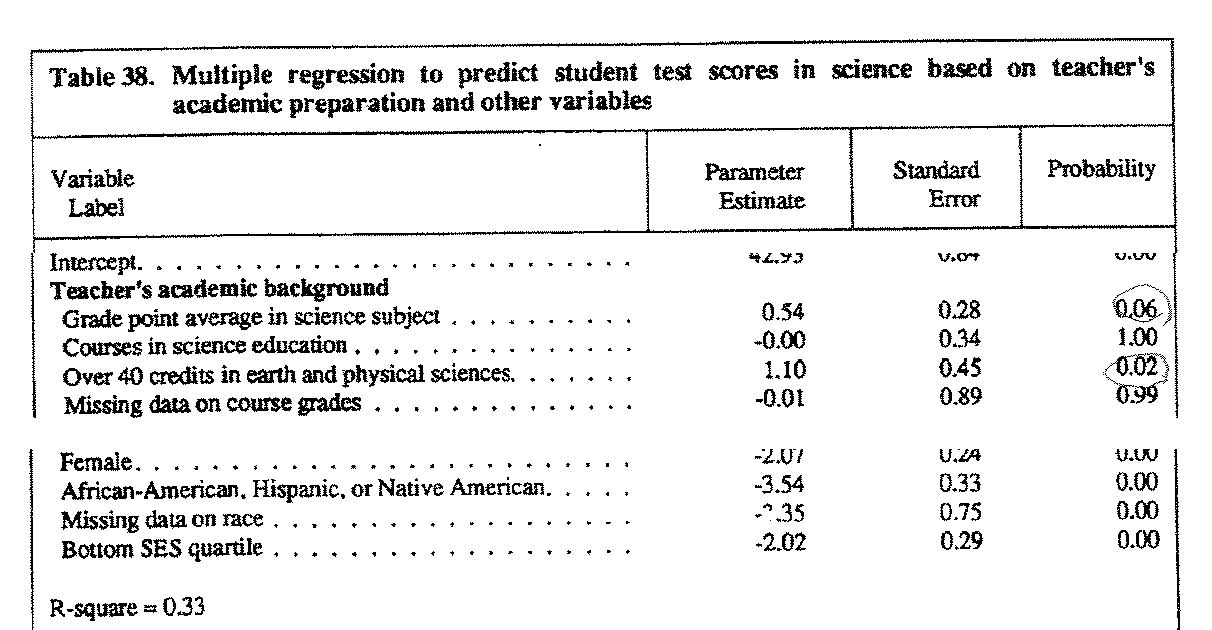
\includegraphics[width=0.9\linewidth]{f_chaney95_regtab.png}
    
  \citep[Quelle:][74; die Tabelle ist nicht vollständig dargestellt]{chaney_student_1995}
  
\end{frame}


\begin{frame}[plain]
  \frametitle{Beispiel semi-partieller Korrelationskoeffizient}
  
  Dem Tabellenausschnitt auf Folie \pageref{slide:chaney-tab} lassen sich
  folgende Informationen für den Effekt von "`Grade point average in science
  subject"' entnehmen:

  \begin{itemize}
  \item $t$-Statistik: 0.54/0.28=1.93
  \item $r_Y^2$ (R-square): 0.33
  \item N (nicht in Tabelle, siehe Fußnote)\footnote{Aloe \& Becker verwenden
      vermutlich die falsche Fallzahl (richtig: 24599), siehe
      \url{http://nces.ed.gov/pubs94/94378.pdf}, Fußnote 3}:
    26435
  \item p (Anzahl Prädiktoren): 26
  \end{itemize}
  
  Dann berechnet sich $r_{sp}$ nach (trotz kleinerer Fehler in Aloe \& Becker
  halte ich mich weitgehend an deren Darstellung):
  
  \begin{equation*}
    r_{sp}=\frac{1.9\sqrt{(1-0.33)}}{\sqrt{(26435-26-1)}}=0.0097
  \end{equation*}
    
  \citep[Quelle: ][346; kleine Typo in Beispielrechnung, $p=26$, nicht
  27]{aloe_advances_2011}
  
\end{frame}


\begin{frame}
  \frametitle{Beispiel Varianz des semi-partiellen Korrelationskoeffizienten}

  Zur Berechnung der Varianz von $r_{sp}$ fehlt noch $r^2_{Y(f)}$, d.h. die
  erklärte Gesamtvarianz für ein Modell \emph{ohne} den \emph{focal predictor}. 
  
  \begin{equation*}
    r^2_{Y(f)}=r^2_Y - r^2_{sp} = 0.33 - 0.0097^2 = 0.3299
  \end{equation*}
  
  Für die Varianz von $r_{sp}$ gilt dann:
  
  \begin{equation*}
    V_{r_{sp}} = \frac{0.1089 - 2 \cdot 0.33 + 0.3299 + 1 - 0.1088}{26435} = 
    0.000025 
  \end{equation*}
    
  Der Standardfehler beträgt:
  
  \begin{equation*}
    SE_{r_{sp}}=0.005
  \end{equation*}
  
  \citep[Quelle: ][347]{aloe_advances_2011}
  
\end{frame}



\subsection{Effektstärkenkonvertierung}

\begin{frame}
  \frametitle{Überblick}
  
  \begin{itemize}
  \item Unterschiedliche Studien berichten trotz gleicher/ähnlicher
    Fragestellung unterschiedliche Statistiken/Effektstärken.
  \item Viele bivariate Effektstärken lassen sich (approximativ) ineinander
    überführen.
  \item Anschließend lassen sich diese konvertierten Effektstärken gemeinsam im
    Rahmen einer Meta-Analyse analysieren.
  \item Hier wird nur eine kleine Auswahl gängiger Transformationsregeln
    vorgestellt. Weiterführende Darstellungen finden sich u.a. bei
    \begin{itemize}
    \item \citet{borenstein_introduction_2009},
    \item \citet{rosenthal_contrasts_2000},
    \item \citet{lipsey_practical_2001},
    \item \citet{higgins_cochrane_2008},
      \item \ldots
    \end{itemize}
  \item Die nachfolgenden Ausführungen basieren auf \citet[46ff.]{borenstein_introduction_2009}.
  \end{itemize}
\end{frame}


\begin{frame}
  \frametitle{Konvertierung zwischen $ln(\text{odds ratio})$ und $d$}

  \begin{equation}
    d = \ln(\text{odds ratio}) \cdot \frac{\sqrt{3}}{\pi}
  \end{equation}
  
  \begin{equation}
    V_d = V_{ln(\text{odds ratio})} \cdot \frac{3}{\pi^2}
  \end{equation}
  
  \begin{equation}
    \ln(\text{odds ratio})=d\frac{\pi}{\sqrt{3}}
  \end{equation}

    \begin{equation}
    V_{ln(\text{odds ratio})} = V_d \frac{\pi^2}{3}
  \end{equation}  

\citep[46ff]{borenstein_introduction_2009}
      
\end{frame}


\begin{frame}
  \frametitle{Konvertierung zwischen $r$ und $d$}

  \begin{equation}
    d = \frac{2r}{\sqrt{1-r^2}}
  \end{equation}
  
  \begin{equation}
    V_d = \frac{4V_r}{(1-r^2)^3}
  \end{equation}
  
  \begin{equation}
    r = \frac{d}{\sqrt{d^2+a}},
  \end{equation}
  
  wobei $a$ ein Korrekturfaktor für $n_1 \neq n_2$ ist:
  
  \begin{equation}
    a = \frac{(n_1+n_2)^2}{n_1n_2}
  \end{equation}
  
  \begin{equation}
    V_r = \frac{a^2V_d}{(d^2+a)^3}
  \end{equation}

  \citep[46ff]{borenstein_introduction_2009}
  
\end{frame}

  



%%% Local Variables:
%%% TeX-master: "ps2012gesis-ma-workshop.tex"
%%% End:



%1
\part{Statistische Verfahren der Meta-Analyse}\label{part:datenanalyse}

\frame{\partpage}

\frame[allowframebreaks]{\frametitle{Statistische Verfahren der Meta-Analyse}
  \begin{footnotesize}\tableofcontents[part=4, hideallsubsections]\end{footnotesize}}

\begin{frame}
  \frametitle{Meta-Analyse auf einen Blick}
  \begin{enumerate}
  \item \emph{Ein} Ziel einer Meta-Analyse ist das Zusammenfassen einer
    Effektstärkenverteilung (ESV) mit Hilfe einer (gewichteten) mittleren ES.
  \item Die Wahl des Schätzverfahrens hängt u.a. vom Ausmaß der Unterschiede
    (Heterogenität, siehe ausführlich \pageref{fr:heterodef}) zwischen
    den ES ab. Es werden (im univariaten Fall) zwei ES-Modelle unterschieden:
    (1) Fixed-effects model (geringe Unterschiede), (2) Random-effects model
    (große Unterschiede).
  \item Neben der Bestimmung eines Mittelwertes geht es in MA \emph{auch/vor
      allem} um die Darstellung/Erfassung und Aufklärung der ES-Heterogenität
    (Regressionsmodelle oder ANOVA-ähnliche Modelle).
  \end{enumerate}
\end{frame}



\section{Befundsynthese von Aggregatdaten}


\begin{frame}
  \frametitle{Befundsynthese} Die Befundsynthese von Aggregatdaten ist ein
  typischer Anwendungsfall einer Meta-Analyse. Dabei sind die folgenden drei
  Bedingungen zu beachten:
  %
  \begin{enumerate}
  \item Die Bildung eines synthetischen Befundes ist nur sinnvoll, wenn
    mindestens zwei einzelne Statistiken berichtet werden,
  \item diese müssen i.A. statistisch unabhängig\footnote{Für abhängige Effektstärken
      gibt es spezielle Verfahren, siehe Folie \pageref{slide:abhaeng-es}.} sein und
  \item in die Mittelwertbildung gehen die einzelnen Befunde nach dem Kriterium
    ihrer Reliabilität (Fehlervarianz/quadrierter SE; Fallzahl) gewichtet ein.
  \end{enumerate}
\end{frame}



\begin{frame}
  \frametitle{Effektstärkenverteilungen beschreiben}
  \begin{itemize}
  \item Ziel ist es, den Lageparameter ("`Mittelwert"') einer ES-Verteilung zu schätzen.
  \item Schätzung ist mit stat. Unsicherheit verbunden, u.a. sind Informationen der
    SEs der einzelnen Effektstärken zu berücksichtigen.
  \item Möglicherweise aber ist die ES-Verteilung durch (unbekannte) Faktoren wie Alter
    oder Geschlecht beeinflusst, d.h. überzufällige Unterschiede zwischen
    Effektstärkengruppen.
  \item Diese Heterogenität/Zwischenstudienvariation beeinflusst die Schätzung
    des Mittelwertes und der stat. Unsicherheit.
  \item Eine zentrale Frage: Ist die ES-Heterogenität so groß, dass wir sie
    berücksichtigen müssen?
    \begin{itemize}
    \item Nein: Fixed-effects model
    \item Ja: Random-effects model
    \end{itemize}
  \end{itemize}
\end{frame}






\subsection{Fixed-effects model (FEM)}

\begin{frame}
  \frametitle{Das \emph{fixed-effects model} (FEM)}
  %%
  \begin{itemize}
  \item Annahmen
    \begin{itemize}
    \item Es gibt \emph{einen} gemeinsamen (\emph{common effect})
      Populationsparameter ($\theta$).
    \item Alle Studien sind sich sehr ähnlich (Design, Stichprobe, Operationalisierung, \ldots).
    \item Es gibt statische Belege für die Homogenität der Effektstärken (Test
      auf Heterogenität), d.h. es gibt keine (kaum) unbeobachtete Heterogenität.
    \item Man kan sich sicher sein, die allermeisten Publikationen entdeckt zu
      haben.
    \end{itemize}
  \item Konsequenzen
    \begin{itemize}
    \item Der Populationsparameter kann relativ genau geschätzt werden (kleiner
      Standardfehler, enges Konfidenzintervall).
    \item Studien mit großen Fallzahlen werden stark gewichtet.
    \end{itemize}
  \end{itemize}
\end{frame}



\begin{frame}
  \frametitle{Verteilung der wahren Effekte im FEM}
  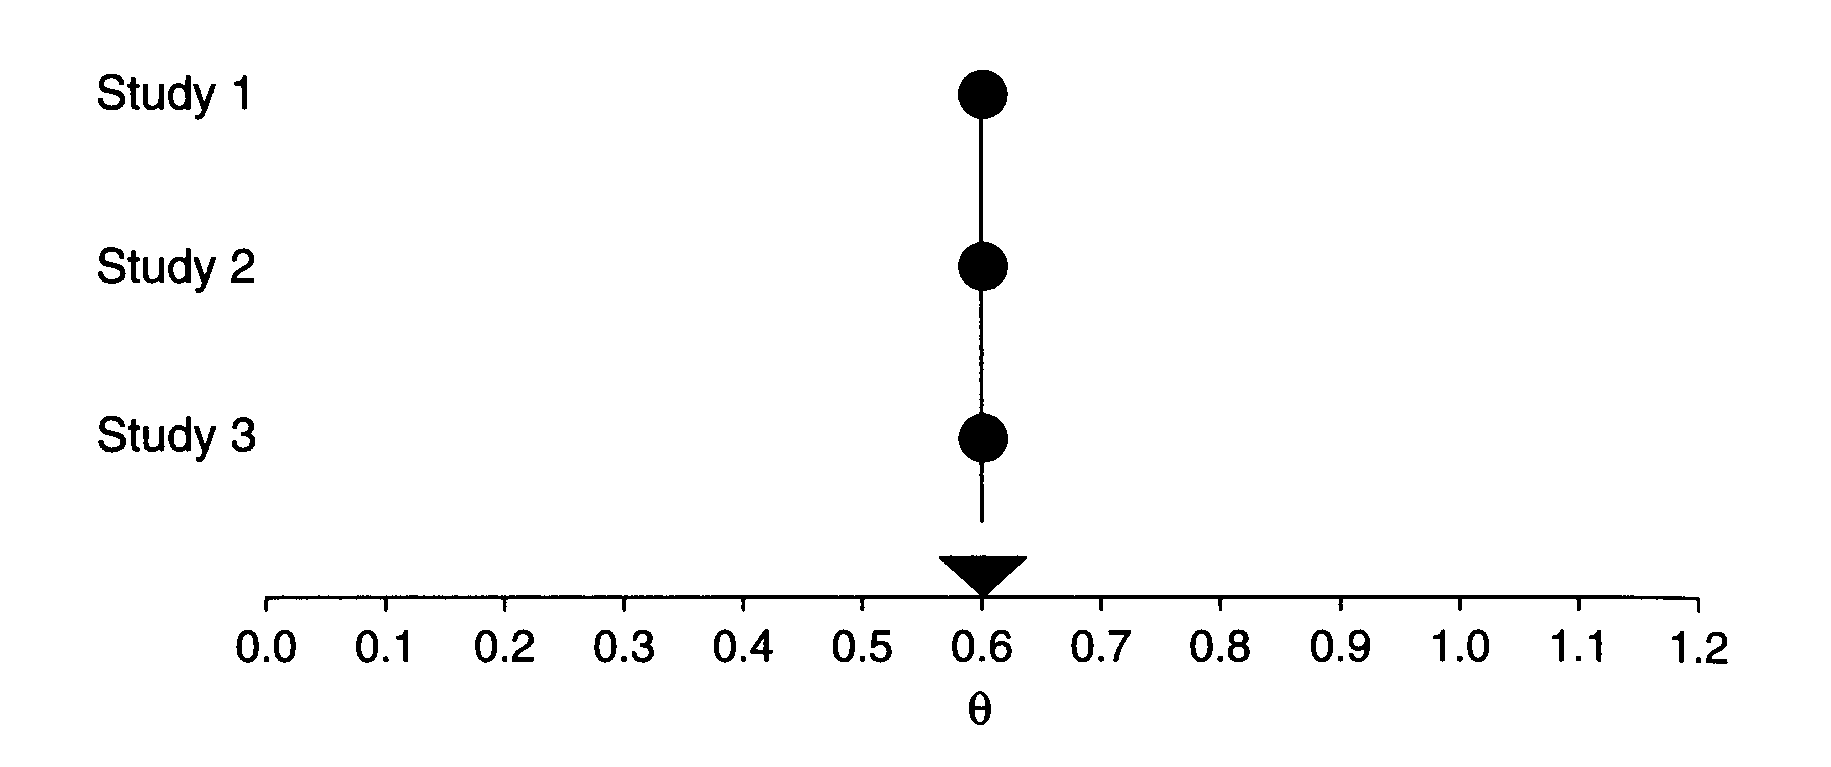
\includegraphics[width=\textwidth]{Borenstein1}
  \newline
  Legende:
  \begin{itemize}
  \item[\FilledSmallCircle] Wahre Effektstärke in Studie $j$
  \item[\FilledSmallTriangleDown] Wahre Effektstärke über alle Studien
    (combined) ($\theta_1 = \theta_2 = \ldots = \theta$)
  \end{itemize}
  \citep[Quelle: ][64]{borenstein_introduction_2009}
\end{frame}


\begin{frame}[shrink = 5]
  \frametitle{Fehler im FEM}
  \includegraphics[width=\textwidth]{Borenstein2}
  \newline
  %%Legende: \FilledSmallCircle, \FilledSmallSquare, \FilledSmallTriangleDown, \FilledSmallDiamondshape
  Legende:
  \begin{itemize}
  \item[\FilledSmallCircle] Wahre Effektstärke in Studie $j$
  \item[\FilledSmallTriangleDown] Wahre Effektstärke über alle Studien
    (combined) ($\theta_1 = \theta_2 = \ldots = \theta$)
  \item[\FilledSmallSquare] Empirische/Beobachtete Effektstärken
  \end{itemize}
  \citep[Quelle: ][64]{borenstein_introduction_2009}
\end{frame}


\begin{frame}[shrink = 5]
  \frametitle{Befundsynthese von Aggregatdaten (FEM)}
  %%
  Gegeben seien $k$ unabhängige Effektstärken $T_j$ ($j = 1, \ldots,k$), dann
  berechnet sich die gewichtete mittlere Effektstärke nach:
  \begin{equation}
    \overline{T}_{FEM} = \frac{\sum\limits^k_{j=1}{w_j \times T_j}}{\sum\limits^k_{j=1}{w_j}},
  \end{equation}
  mit einem Gewicht $w_j$, das der inversen Fehlervarianz ($1/v_j$) bzw. dem
  inversen quadrierten Standardfehler ($1/SE_j$) der $j$-ten Effektstärke
  entspricht:
  \begin{equation}
    w_j=\frac{1}{SE^2_j} = \frac{1}{v_j}.
  \end{equation}
  Die zusammengefasste Fehlervarianz $\overline{v}_{FEM}$ selbst ergibt sich
  aus:
  \begin{equation}
    \overline{v}_{FEM}=\frac{1}{\sum\limits^k_{j=1}(1/v_j)}.
  \end{equation}
  Für den Standardfehler von $\overline{T}_{FEM}$ gilt dann $\overline{SE}_{FEM}
  = \sqrt{\overline{v}_{FEM}}$.
\end{frame}



\subsection{Random-effects model (REM)}

\begin{frame}[shrink=10]
  \frametitle{Das \emph{random-effects model} (REM)}
  %%
  \begin{itemize}
  \item Annahmen
    \begin{itemize}
    \item Jede Studie $j$ besitzt ihren eigenen Populationsparameter
      ($\theta_j$), geschätzt wird ein "`mittlerer"' Effekt (\emph{average effect}).
    \item Man kann nicht annehmen, dass alle Studien ähnlich sind (Design,
      Stichprobe, Operationalisierung, \ldots).
    \item Es lassen sich u.U. aus der Theorie Einflussgrößen ableiten, die für
      Unterschiede in den Studienbefunden verantwortlich gemacht werden können.
    \item Es gibt statische Belege für die Heterogenität der Effektstärken (Test
      auf Heterogenität).
    \item Man kan sich nicht sicher sein, die allermeisten Publikationen
      entdeckt zu haben.
    \end{itemize}
  \item Konsequenzen
    \begin{itemize}
    \item Der gemeinsame Populationsparameter kann nur ungenau geschätzt werden
      (großer Standardfehler, breites Konfidenzintervall).
    \item Die Studiengewichte werden ähnlicher, d.h. große Studien erhalten
      weniger Einfluss, kleine Studien gewinnen Einfluss.
    \end{itemize}
  \end{itemize}
\end{frame}


\begin{frame}
  \frametitle{Verteilung der wahren Effektstärken im REM}
  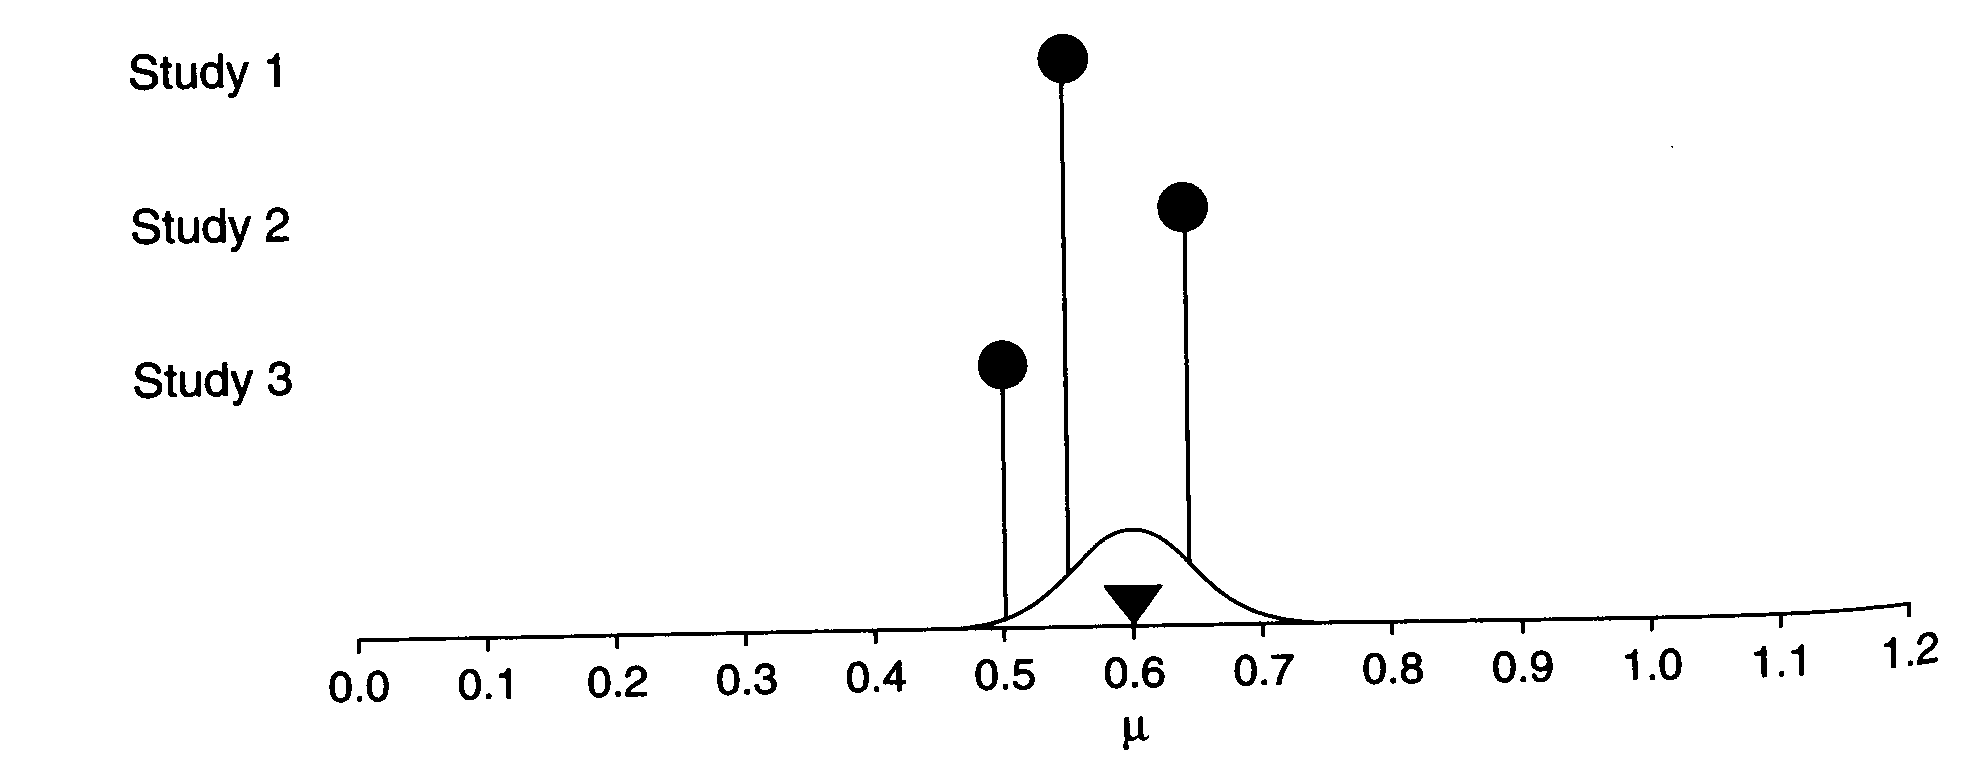
\includegraphics[width=\textwidth]{Borenstein5}
  \newline
  Legende:
  \begin{itemize}
  \item[\FilledSmallCircle] Wahre Effektstärke in Studie $j$
  \item[\FilledSmallTriangleDown] Mittlere ("`average"') Effektstärke über alle
    Studien (combined)
  \end{itemize}
  \citep[Quelle: ][70]{borenstein_introduction_2009}
\end{frame}


\begin{frame}[shrink = 5]
  \frametitle{Fehler im REM}
  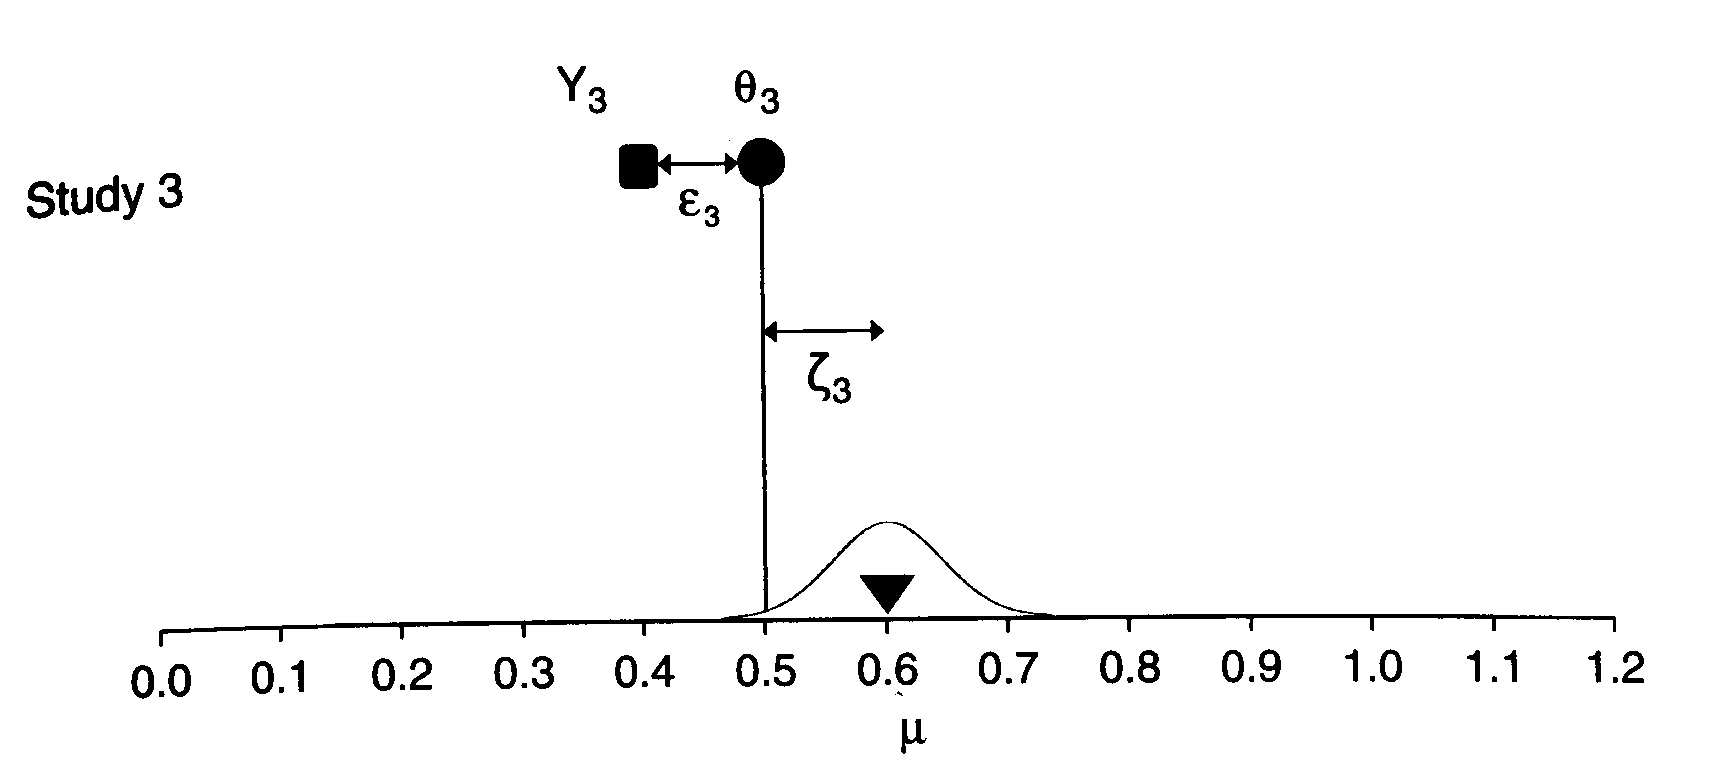
\includegraphics[width=\textwidth]{Borenstein6}
  \newline
  %%Legende: \FilledSmallCircle, \FilledSmallSquare, \FilledSmallTriangleDown, \FilledSmallDiamondshape
  Legende:
  \begin{itemize}
  \item[\FilledSmallCircle] Wahre Effektstärke in Studie $j$
  \item[\FilledSmallSquare] Empirische/Beobachtete Effektstärken
  \item[\FilledSmallTriangleDown] Wahre Effektstärke über alle Studien (combined)
  \item Übersetzung der unterschiedlichen Nomenklatur (siehe Folie \pageref{slide:fem-refm-fehler}): $\zeta_3 = u_3$
  \end{itemize}
  \citep[Quelle: ][71]{borenstein_introduction_2009}
\end{frame}


\begin{frame}[shrink = 5]
  \frametitle{Verteilung der Stichprobenfehler im REM: Binnen- und Zwischenstudienvarianz}
  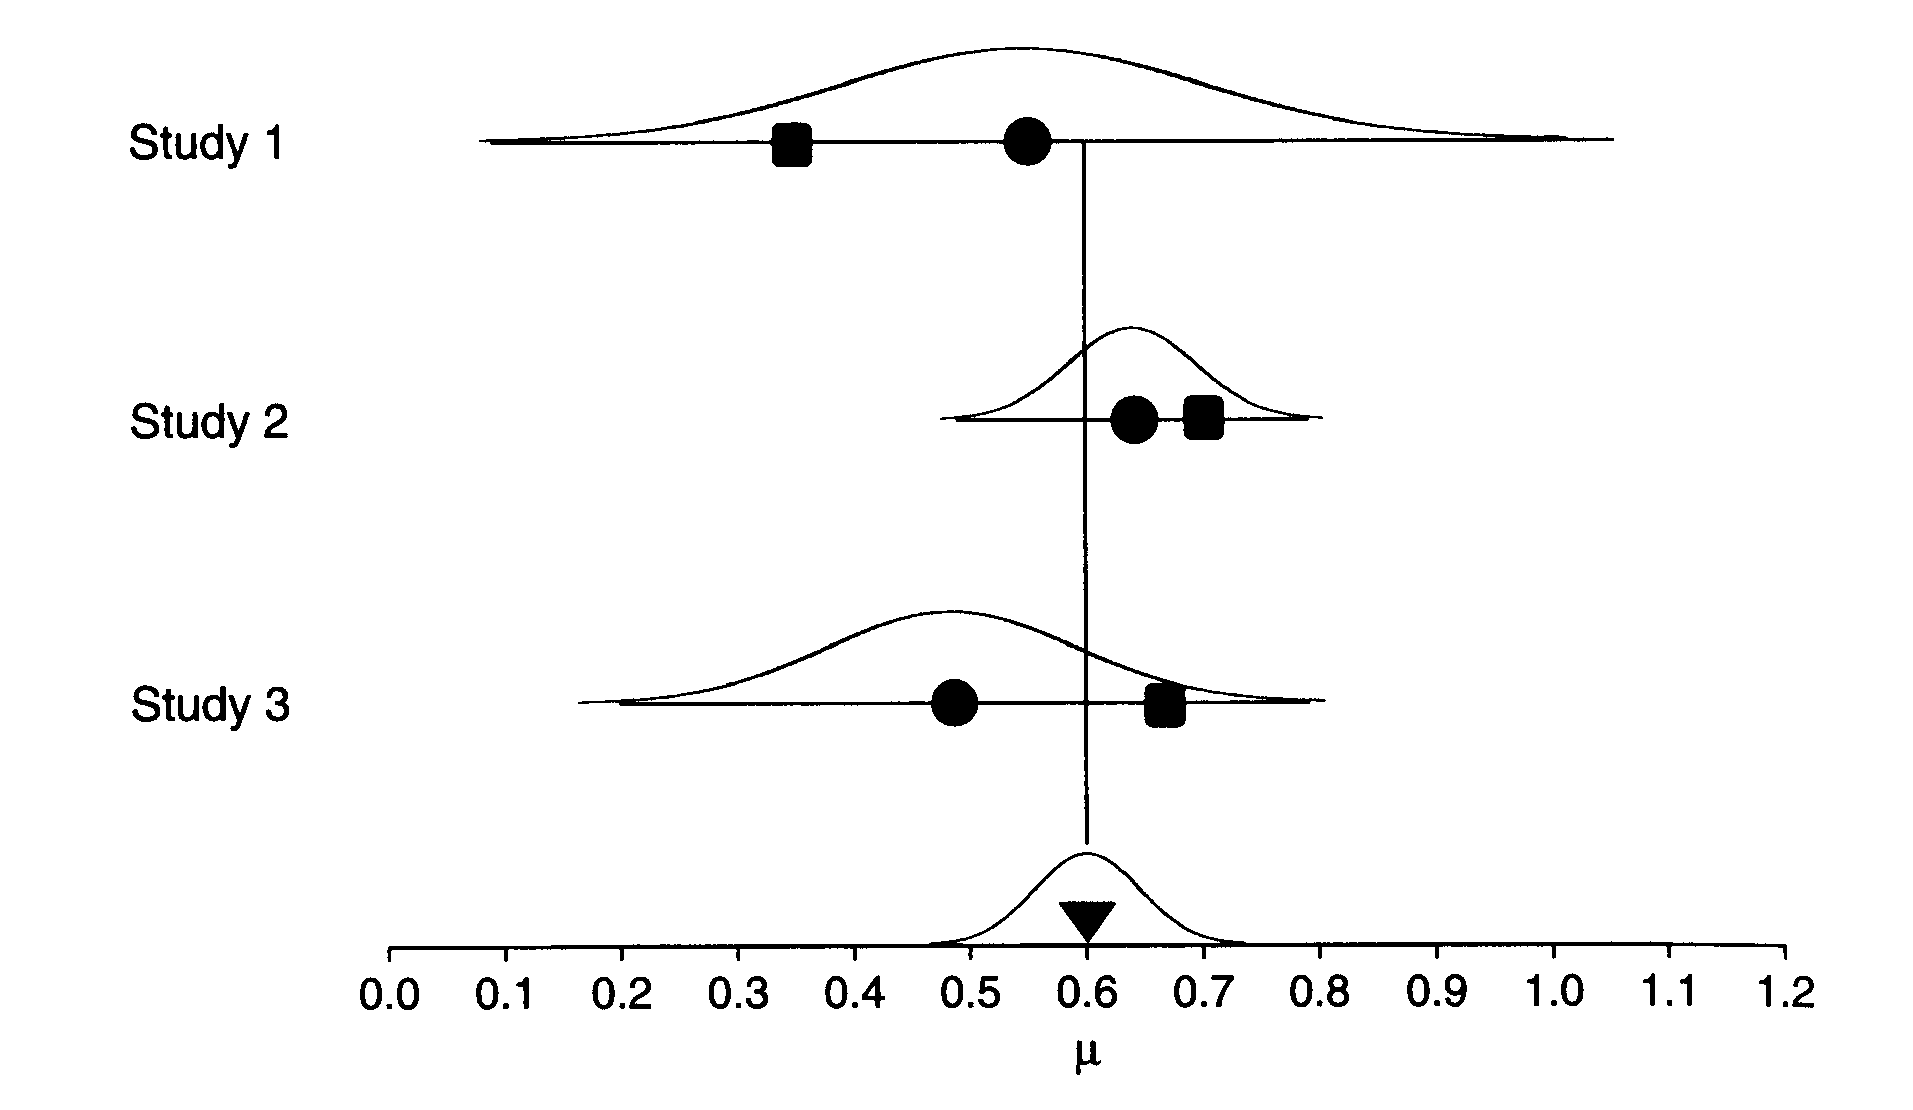
\includegraphics[width=\textwidth]{Borenstein7}
  \newline
  %%Legende: \FilledSmallCircle, \FilledSmallSquare, \FilledSmallTriangleDown, \FilledSmallDiamondshape
  Legende:
  \begin{itemize}
  \item[\FilledSmallCircle] Wahre Effektstärke in Studie $j$
  \item[\FilledSmallSquare] Empirische/Beobachtete Effektstärken (Hinweis: Studie 1 kleines N, Studie 2 großes N)
  \item[\FilledSmallTriangleDown] Mittlere ("`average"') Effektstärke über alle Studien (combined)
  \end{itemize}
  \citep[Quelle: ][71]{borenstein_introduction_2009}
\end{frame}


\begin{frame}[plain]
  \frametitle{Das REM als ein zweistufiger Prozess}
  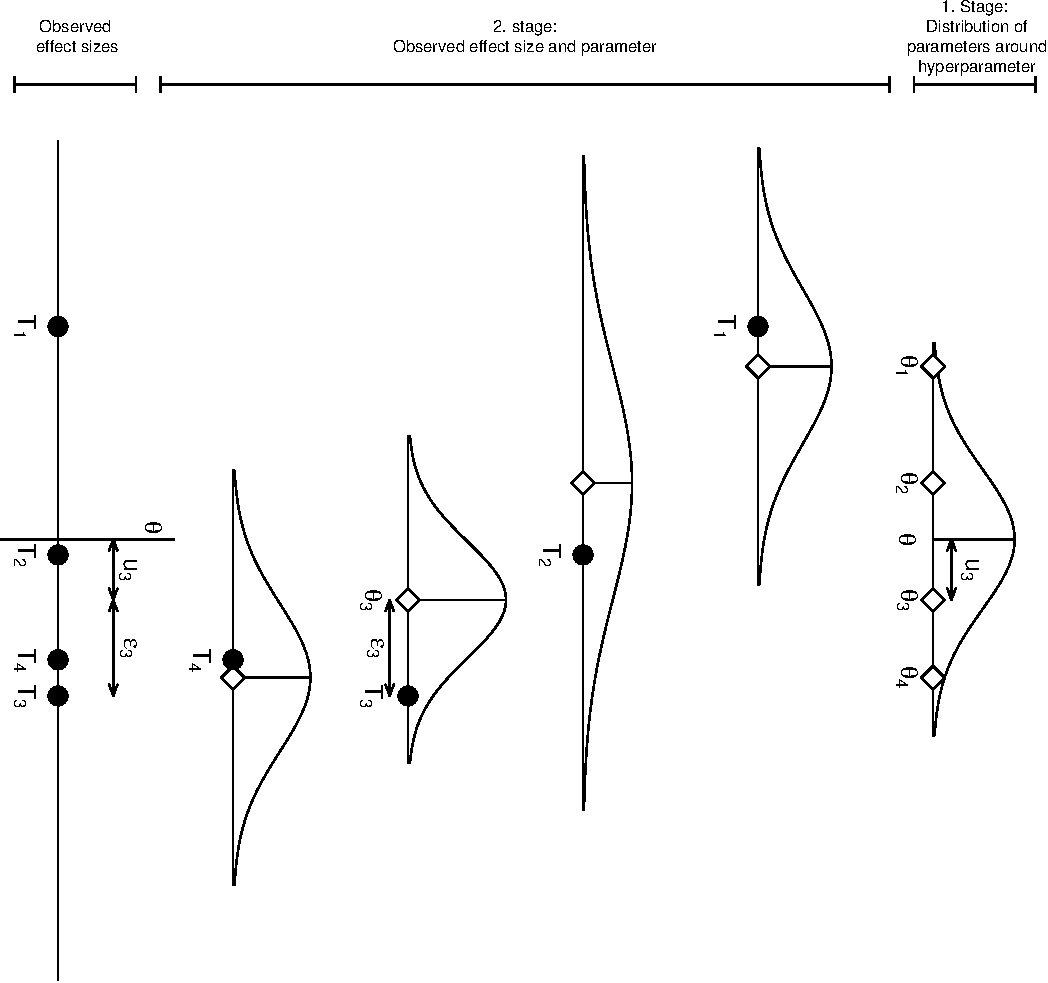
\includegraphics[width=0.71\textwidth, angle=90]{f_rem_diagram2}


\citep[Quelle: ][]{thompson_introduction_2013, viechtbauer_accounting_2007}

%(Source: Thompson/Weiß 2013)

\end{frame}




\begin{frame}
  \frametitle{Vergleich von FEM und REM}
  \begin{itemize}[<+->]
  \item Gilt das FEM, dann liegt allen Studien ein gemeinsames $\theta$
    zugrunde. Studien mit kleinen Fallzahlen werden durch das Heruntergewichten
    weitgehend ignoriert, da in umfangreichen Studien bessere Informationen über
    $\theta$ vorliegen.
  \item Dagegen wird im REM der Mittelwert einer Effektstärkenverteilung
    geschätzt ("`mean of a distribution of effects"'). Kleine Studien sind daher
    wichtiger als im FEM und erhalten mehr Gewicht.
  \end{itemize}
\end{frame}


\begin{frame}[shrink=5]
  \frametitle{Fehlerterme im FEM und REM}\label{slide:fem-refm-fehler}
  \begin{small}
    \begin{block}{Fixed-effects model}
      \begin{equation*}\label{eq:hlm-level1fem}
        T_j = \theta + \epsilon_{j}
      \end{equation*}
      Alle Befundstatistiken $T_j$ entstammen \emph{einer} Population ($\theta$).
      %% \item Keine Berücksichtigung möglicher Zwischenstudienvarianz.
    \end{block}
    %%
    \pause
    \begin{block}{Random-effects model}
      \begin{eqnarray*}
        T_j & = & \theta_j + \epsilon_{j} \\
        \theta_j & = & \theta + u_j \\
        \Rightarrow  T_j & = & \theta + \epsilon_{j} + u_j
      \end{eqnarray*}
      \begin{itemize}
      \item Pro Befundstatistik $T_j$ ein je eigener Populationsparameter
        $\theta_j$; alle $\theta_j$ wiederum streuen um den Parameter
        $\theta$ einer "`Superpopulation"'.
      \item Berücksichtigung der Zwischenstudienvarianz $Var(u_j)=\tau^2$, so
        dass $w^*_j = \frac{1}{v_j^*} = \frac{1}{v_j+\tau^2}$.
      \end{itemize}

      \end{block}
  \end{small}
\end{frame}


\begin{frame}[plain]
  \frametitle{Schätzen der Zwischenstudienvarianz $\tau^2$}

  Der sog. Momentenschätzer für $\tau^2$ lautet:

  \begin{equation}
    \widehat{\tau}^2 = \frac{Q-(k-1)}{c} =  \frac{Q-df}{c}
  \end{equation}

  mit:\\
  $k$: Anzahl der Effektstärken\\
  $df$: Anzahl der Freiheitsgrade ($df = k-1$)\\
  $Q$: Maß der Zwischenstudienvariation, $Q \sim \chi_{df}^2$
       (Heterogenitätstest, siehe ausführlich Folie \pageref{sec:die-q-statistik}) \\
  $c$: Skalierungsfaktor, sorgt dafür, dass $\tau^2$ wieder die Metrik der
  Ausgangs-ES erhält.

  \begin{equation}
    Q = \sum\limits^k_{j = 1}\left(\frac{(T_j - \overline{T}_{FEM})^2}{v_i}\right)
  \end{equation}

  Für eine ausführlichere Darstellung der Zwischenstudienvarianz siehe Folien \pageref{sec:tau}ff.

\end{frame}



\begin{frame}
  \frametitle{Befundsynthese von Aggregatdaten (REM)}
  %%
  Gegeben seien $k$ unabhängige Effektstärken $T_j$ ($j = 1, \ldots,k$), dann
  berechnet sich die gewichtete mittlere Effektstärke nach dem \emph{random-effects model} nach:
  \begin{equation}
    \overline{T}_{REM} = \frac{\sum\limits^k_{j=1}{w^*_j \times T_j}}{\sum\limits^k_{j=1}{w^*_j}},
  \end{equation}
  mit einem Gewicht $w^*_j$, für das gilt: $w^*_j = \frac{1}{v_j^*} = \frac{1}{v_j+\widehat{\tau}^2}$.

  Die Gesamtfehlervarianz (bzw. der Standardfehler) für den REM-Schätzer ergib
  sich nach:
  \begin{equation*}
    \overline{v}_{REM} = \frac{1}{\sum^k_{j=1}w^*_j} \text{ bzw. }  \overline{SE}_{REM} = \frac{1}{\sqrt{\sum^k_{j=1}w^*_j}}
  \end{equation*}
\end{frame}







\begin{frame}[fragile, plain]\frametitle{Beispiel "`Teacher verbal ability \&
    school outcomes"'}
\begin{footnotesize}
\begin{knitrout}
\definecolor{shadecolor}{rgb}{0.827, 0.827, 0.827}\color{fgcolor}\begin{kframe}
\begin{verbatim}
       r        z    se.z
1  -0.10 -0.10034 0.50000
5  -0.09 -0.09024 0.18898
7  -0.07 -0.07011 0.11471
3  -0.05 -0.05004 0.08111
13 -0.05 -0.05004 0.18898
9  -0.01 -0.01000 0.08220
4   0.02  0.02000 0.15430
11  0.03  0.03001 0.05634
15  0.03  0.03001 0.04486
8   0.04  0.04002 0.08220
12  0.07  0.07011 0.05923
10  0.12  0.12058 0.12804
14  0.13  0.13074 0.04486
16  0.21  0.21317 0.04486
2   0.23  0.23419 0.11704
6   0.26  0.26611 0.17150
17  0.28  0.28768 0.04486
\end{verbatim}
\end{kframe}
\end{knitrout}

\end{footnotesize}
\citep[Quelle: ]{aloe_teacher_2009}
\end{frame}


\begin{frame}[fragile, shrink=15, plain]\frametitle{Beispiel "`Teacher verbal
    ability \& school outcomes: Forestplot}

\begin{knitrout}
\definecolor{shadecolor}{rgb}{0.827, 0.827, 0.827}\color{fgcolor}
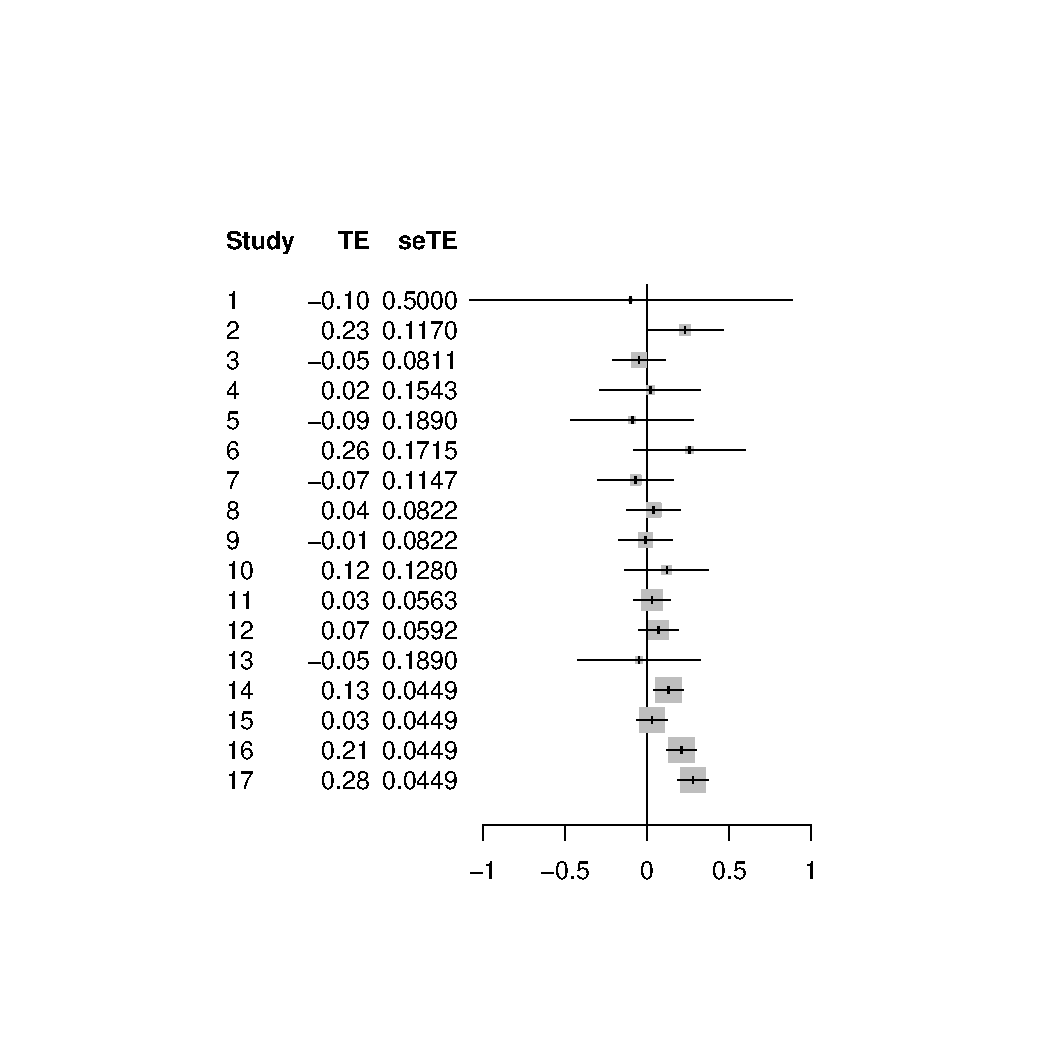
\includegraphics[width=\textwidth]{fig/forestverbab} 

\end{knitrout}

\end{frame}




\begin{frame}[fragile, plain, shrink]\frametitle{Beispiel "`Teacher verbal
    ability \& school outcomes"': FEM und REM}

  \begin{tiny}
\begin{knitrout}
\definecolor{shadecolor}{rgb}{0.827, 0.827, 0.827}\color{fgcolor}\begin{kframe}
\begin{verbatim}
                       95%-CI %W(fixed) %W(random)
1  -0.1003  [-1.0803; 0.8796]      0.12       0.38
2   0.2342  [ 0.0048; 0.4636]      2.16       4.52
3  -0.0500  [-0.2090; 0.1089]      4.49       6.72
4   0.0200  [-0.2824; 0.3224]      1.24       3.09
5  -0.0902  [-0.4606; 0.2802]      0.83       2.25
6   0.2661  [-0.0700; 0.6022]      1.01       2.63
7  -0.0701  [-0.2949; 0.1547]      2.25       4.64
8   0.0400  [-0.1211; 0.2011]      4.38       6.63
9  -0.0100  [-0.1711; 0.1511]      4.38       6.63
10  0.1206  [-0.1304; 0.3715]      1.80       4.02
11  0.0300  [-0.0804; 0.1404]      9.31       8.74
12  0.0701  [-0.0460; 0.1862]      8.43       8.49
13 -0.0500  [-0.4204; 0.3204]      0.83       2.25
14  0.1307  [ 0.0428; 0.2187]     14.70       9.75
15  0.0300  [-0.0579; 0.1179]     14.70       9.75
16  0.2132  [ 0.1253; 0.3011]     14.70       9.75
17  0.2877  [ 0.1998; 0.3756]     14.70       9.75

Number of studies combined: k=17

                                       95%-CI     z  p.value
Fixed effect model   0.1123  [0.0786; 0.1460] 6.530 < 0.0001
Random effects model 0.0880  [0.0265; 0.1495] 2.803   0.0051

Quantifying heterogeneity:
tau^2 = 0.0081; H = 1.59 [1.22; 2.07]; I^2 = 60.4% [32.6%; 76.7%]

Test of heterogeneity:
     Q d.f.  p.value
 40.36   16   0.0007

Details on meta-analytical method:
- Inverse variance method
- DerSimonian-Laird estimator for tau^2
\end{verbatim}
\end{kframe}
\end{knitrout}

\end{tiny}
\end{frame}


\section{Begriff der Heterogenität und Diagnostik}


\subsection{Überblick}\label{sec:heteroueberblick}

\begin{frame}
  \frametitle{Ist Heterogenität ein Problem?}\label{fr:heterodef}
  %%
  \begin{itemize}[<+->]
  \item<+-> Die ES-Synthese ist eine (relativ) einfache Operation.
  \item<+-> Ist diese mittlere ES eine angemessene Zusammenfassung der
    zugrunde liegenden Verteilung?
  \item<+-> Das hängt u.a. von der "`Gesamtvariation"' der ES ab:
    \begin{itemize}
    \item Die Gesamtvariation lässt sich in zwei Teile zerlegen: (1) Stichprobenfehler ("`random error"';
      "`within-study error"'), (2) "`wahre"' Streuung ("between study error"', "`heterogeneity"')
    \item "`[...] we use \emph{heterogeneity} to mean heterogeneity in true effects only"' (Borenstein et al 2009: 106).
    \end{itemize}
\item<+-> Ziel der Heterogenitätsdiagnostik ist u.a. das Ausmaß der "`wahren"' Streuung zu bestimmen.
  \end{itemize}
\end{frame}

\begin{frame}[plain]
  \frametitle{Schätzen Sie mal \ldots}
  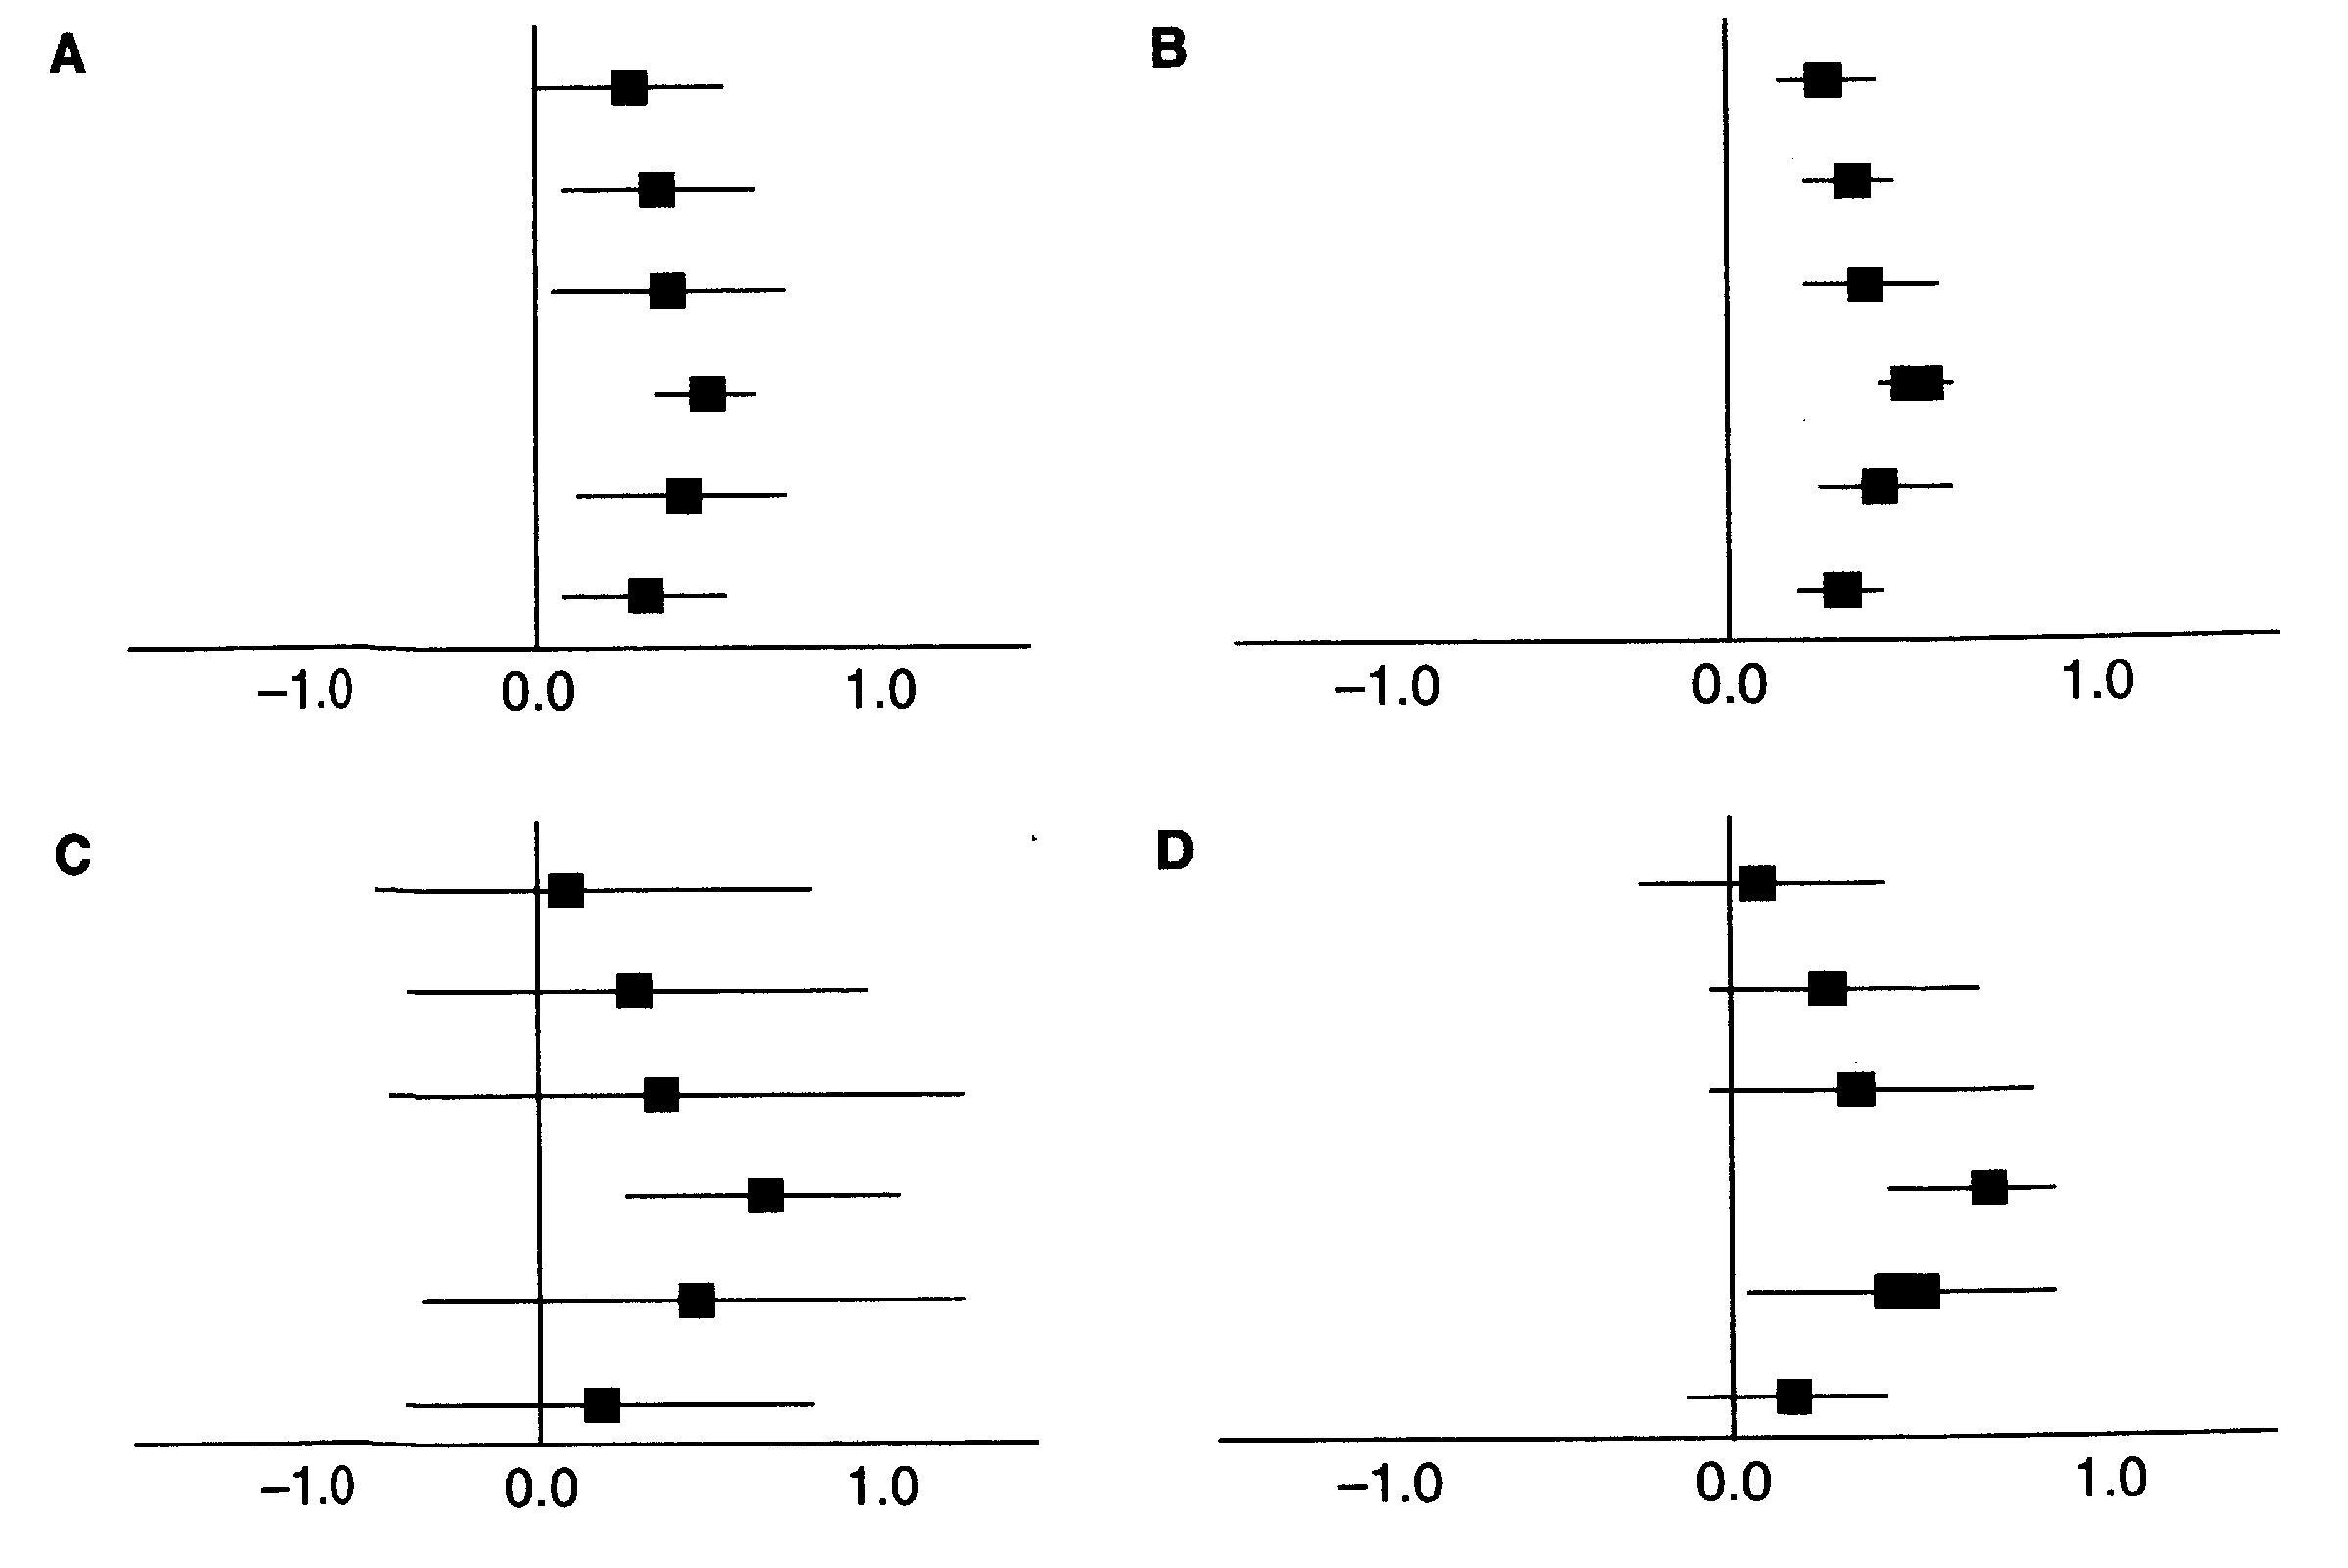
\includegraphics[width=\textwidth]{borenstein108}
\newline(Quelle: Borenstein et al. 2009: 108)
\end{frame}


\begin{frame}[shrink = 5]
  \frametitle{Schätzen Sie mal \ldots die Auflösung}
  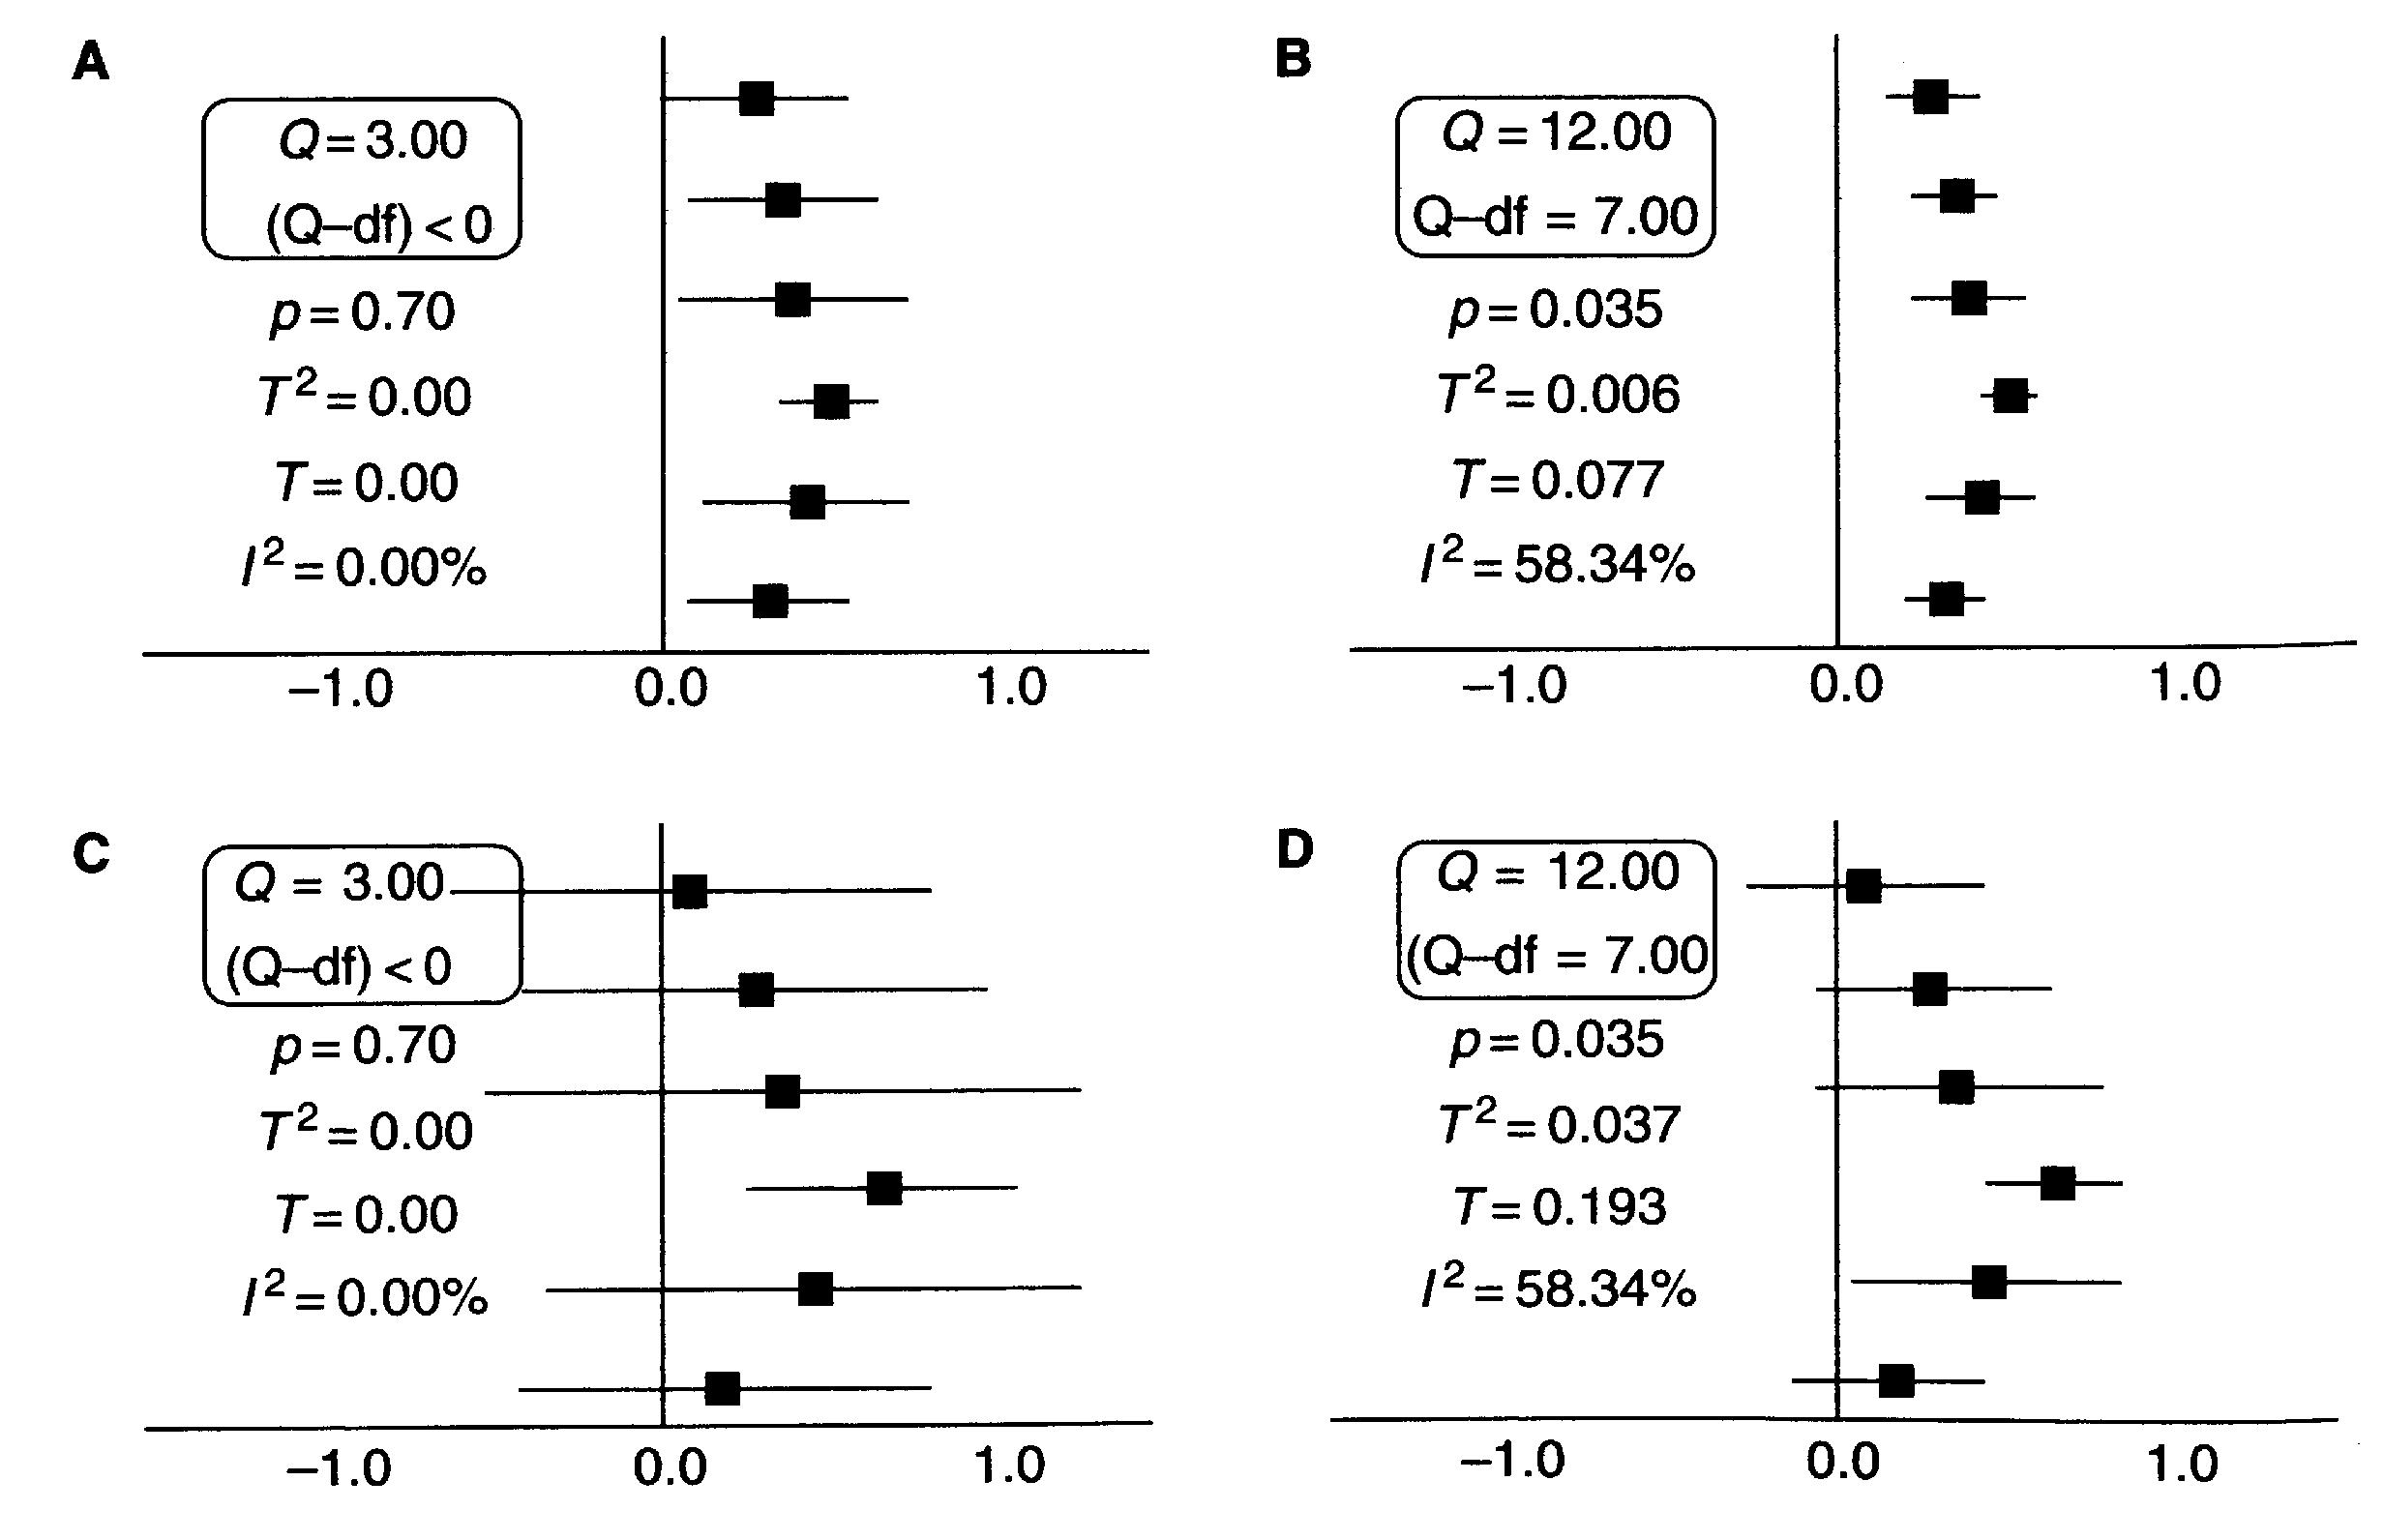
\includegraphics[width=\textwidth]{borenstein110}
\newline(Quelle: Borenstein et al. 2009: 110)
\end{frame}


\begin{frame}
  \frametitle{Anliegen und Maße der Heterogenitätsdiagnostik}
  %%
  \begin{itemize}[<+->]
  \item<+-> "`Is there evidence of heterogeneity in true effect sizes? (Q-Test)
  \item<+-> What is the variance of the true effects? ($\tau^2$, $\widehat{\tau}^2 = T^2$)
  \item<+-> What proportion of the observed dispersion is real?"' ($I^2$)
  \end{itemize}

\citep[Quelle: ][105]{borenstein_introduction_2009}
\end{frame}



\subsection{Die Zwischenstudienvarianz}\label{sec:tau}

\begin{frame}
  \frametitle{Die Zwischenstudienvarianz}
  %%
  "`The parameter\footnote{In der Literatur finden sich uneinheitliche Notationen, um die Zwischenstudienvarianz zu
    beschreiben. Teilweise wird keine unterschiedliche Notation verwendet, um zwischen Parameter und Schätzwert zu
    unterscheiden. Teilweise finden sich aber auch folgende Varianten: $\tau^2$ und $\widehat{\tau}^2$ oder $\tau^2$ und
    $T^2$. } tau-squared ($\tau^2$) is defined as the variance of the true effect sizes. In other words, if we had
  an infinitely large sample of studies, each, itself, infinitely large (so that the estimate in each study was the true
  effect) and computed the variance of these effects, this variance would be $\tau^2$"' (Borenstein et al. 2009: 114).
\end{frame}


\begin{frame}
  \frametitle{Wie lässt sich die "`wahre"' Zwischenstudienvarianz isolieren?}

"`The mechanism that we use to extract the true between-studies variation from the observed variation is as follows:

\begin{enumerate}[<+->]
\item<+-> We compute the total amount of study-to-study variation actually observed ($Q$).
\item<+-> We estimate how much the observed effects would be expected to vary from each other if the true effect was
  actually the same in all studies ($k-1 = df$).
\item<+-> The excess variation (if any) is assumed to reflect real differences in effect size (that is, the
  heterogeneity)"' (Borenstein et al. 2009: 108).
\end{enumerate}
\end{frame}



\begin{frame}
  \frametitle{Schätzen der Zwischenstudienvarianz $\tau^2$}

  \begin{footnotesize}
    Der sog. Momentenschätzer\footnote{Für eine Übersicht und einen Vergleich
      verschiedener Schätzer von $\tau^2$ siehe \citet{viechtbauer_bias_2005}.}
    für $\tau^2$ lautet:

  \begin{equation*}
    \widehat{\tau}^2 = \frac{Q-(k-1)}{c} =  \frac{Q-df}{c}
  \end{equation*}

  mit:\\
  $k$: Anzahl der Effektstärken\\
  $df$: Anzahl der Freiheitsgrade ($df = k-1$)\\
  $Q$: Maß der Zwischenstudienvariation, $Q \sim \chi_{df}^2$
  (Heterogenitätstest, siehe ausführlich Folie \pageref{sec:die-q-statistik}) \\
  $c$: Skalierungsfaktor, sorgt dafür, dass $\tau^2$ wieder die Metrik der
  Ausgangs-ES erhält. $c$ berechnet sich nach (zur Erinnerung: $w_i = 1/v_i$):

  \begin{equation}
    c = \sum\limits^k_{j = 1}w_i - \left(\frac{\sum\limits^k_{j = 1}w_i^2}{\sum\limits^k_{j = 1}w_i}\right)
  \end{equation}
\end{footnotesize}
\end{frame}



% \begin{frame}[shrink = 5]
%   \frametitle{Einflussfaktoren von $\tau^2$}
%   \includegraphics[width=\textwidth]{borenstein115}
%   \newline(Quelle: Borenstein et al. 2009: 115)
% \end{frame}


\subsection{Die $Q$- Statistik}\label{sec:die-q-statistik}

\begin{frame}
  \frametitle{Die Heterogenitätsstatistik $Q$}
  %%
  \begin{itemize}
  \item Bestimmen der Gesamtabweichung ("`total amount of study-to-study
    variation"', "`observed weighted sum of squares"' (WSS)):
    \begin{equation}
      Q = \sum\limits^k_{j = 1}\left(\frac{(T_j - \overline{T}_{FEM})^2}{SE_j^2}\right)
    \end{equation}
  \item Erwartete Variation, wenn es keine Zwischenstudienvarianz gäbe (= FEM) (expected WSS):
    \begin{equation}
      df = k-1
    \end{equation}
  \item Ausmaß der Zwischenstudienvariation ("`excess variation"'):
    \begin{equation}
      Q-df
    \end{equation}
  \end{itemize}
\end{frame}


\begin{frame}
  \frametitle{Das Prinzip des $Q$-Tests}
  \begin{itemize}
  \item<+-> Hypothesen:
    \begin{itemize}
    \item $H_0$: Die Effektstärken weisen einen gemeinsamen Populationsparameter auf.
    \item $H_1$: Die Effektstärken weisen mehr als einen gemeinsamen
      Populationsparameter auf.
    \end{itemize}
  \item<+-> Wenn die $H_0$ \emph{nicht} zurückwiesen werden kann, dann wird eine homogene
    Effektstärkenverteilung unterstellt.
  \item<+-> $Q$ ist mit $df = k-1$ Freiheitsgeraden $\chi^2$-verteilt. Für jeden
    Freiheitsgrad lässt sich ein theoretischer $\chi^2$-Wert angeben, der sich
    mit dem empirischen $\chi^2$-Wert ($=Q$) vergleichen lässt. Ist der
    empirische $\chi^2$-Wert größer als der theoretische (= statistisch
    signifikant), dann kann man \emph{keine} homogene Effektstärkenverteilung
    annehmen.
  \end{itemize}
\end{frame}


\begin{frame}
  \frametitle{Hinweise zur Interpretation von $Q$}
  \begin{small}
    \begin{itemize}[<+->]
    \item Der $Q$-Test weist eine niedrige statistische \emph{power} auf, d.h. eine relativ hohe Wahrscheinlichkeit
      einen Fehler 2. Art ($\beta$-Fehler) zu begehen. \emph{Dies gilt vor allem für Meta-Analysen mit kleinen
        Fallzahlen ($k<20$).} Mit anderen Worten: Ein nicht-signifikanter Test belegt nicht unbedingt eine homogene
      Effektstärkenverteilung. Deshalb wird häufig auch ein Signifikanzniveau von $10\%$ angesetzt.

    \item "`[\ldots] [W]hile a significant $p$-value provides evidence that the true effects vary, the converse is not
      true. A nonsignificant $p$-value should not be taken as evidence that the effect sizes are consistent, since the
      lack of significance may be due to low power. With a small number of studies and/or large within-study variance
      (small studies), even substantial between-studies dispersion might yield a nonsignificant $p$-value"' (Borenstein
      et al. 2009: 113).
    \end{itemize}
  \end{small}
\end{frame}

\begin{frame}[shrink = 5]
  \frametitle{Einfluss der Fallzahl auf $Q$ und den $p$-Wert }
  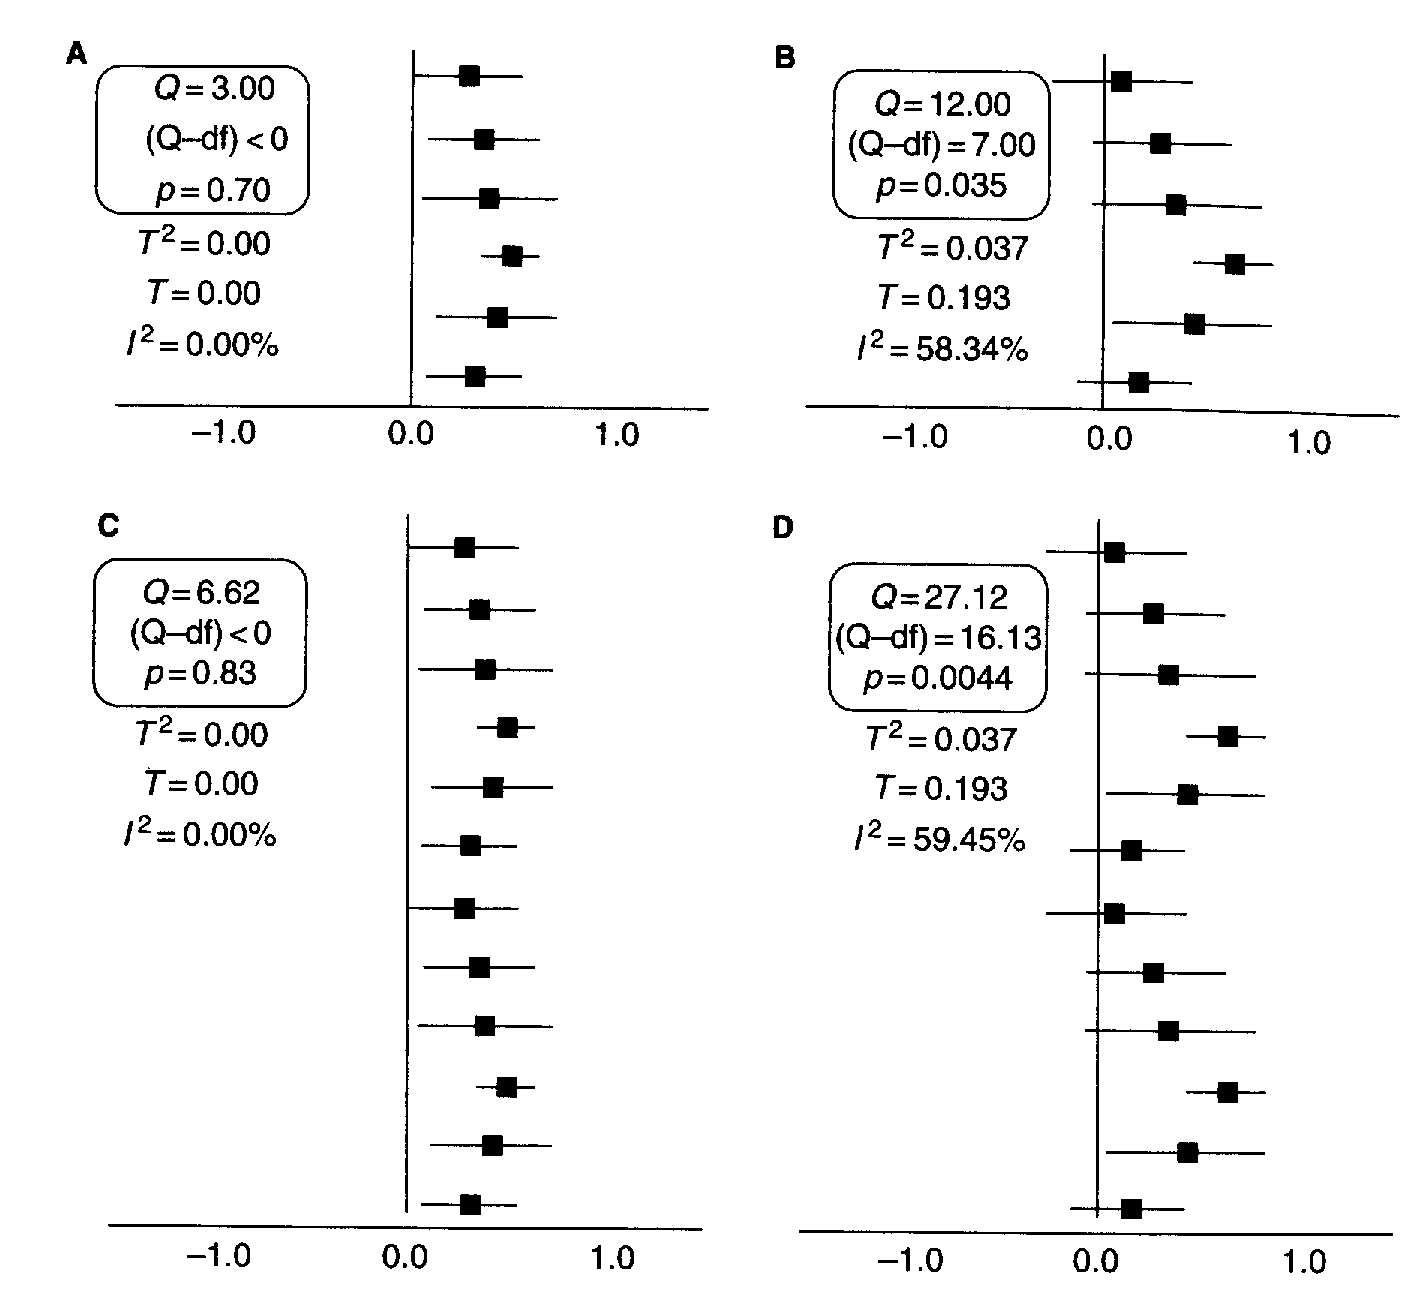
\includegraphics[width=\textwidth]{borenstein113}
\newline(Quelle: Borenstein et al. 2009: 113)
\end{frame}


\begin{frame}[shrink = 5]
  \frametitle{Beispiel für das Verhältnis von Binnen- (within) und Zwischenstudienvarianz (between)}
  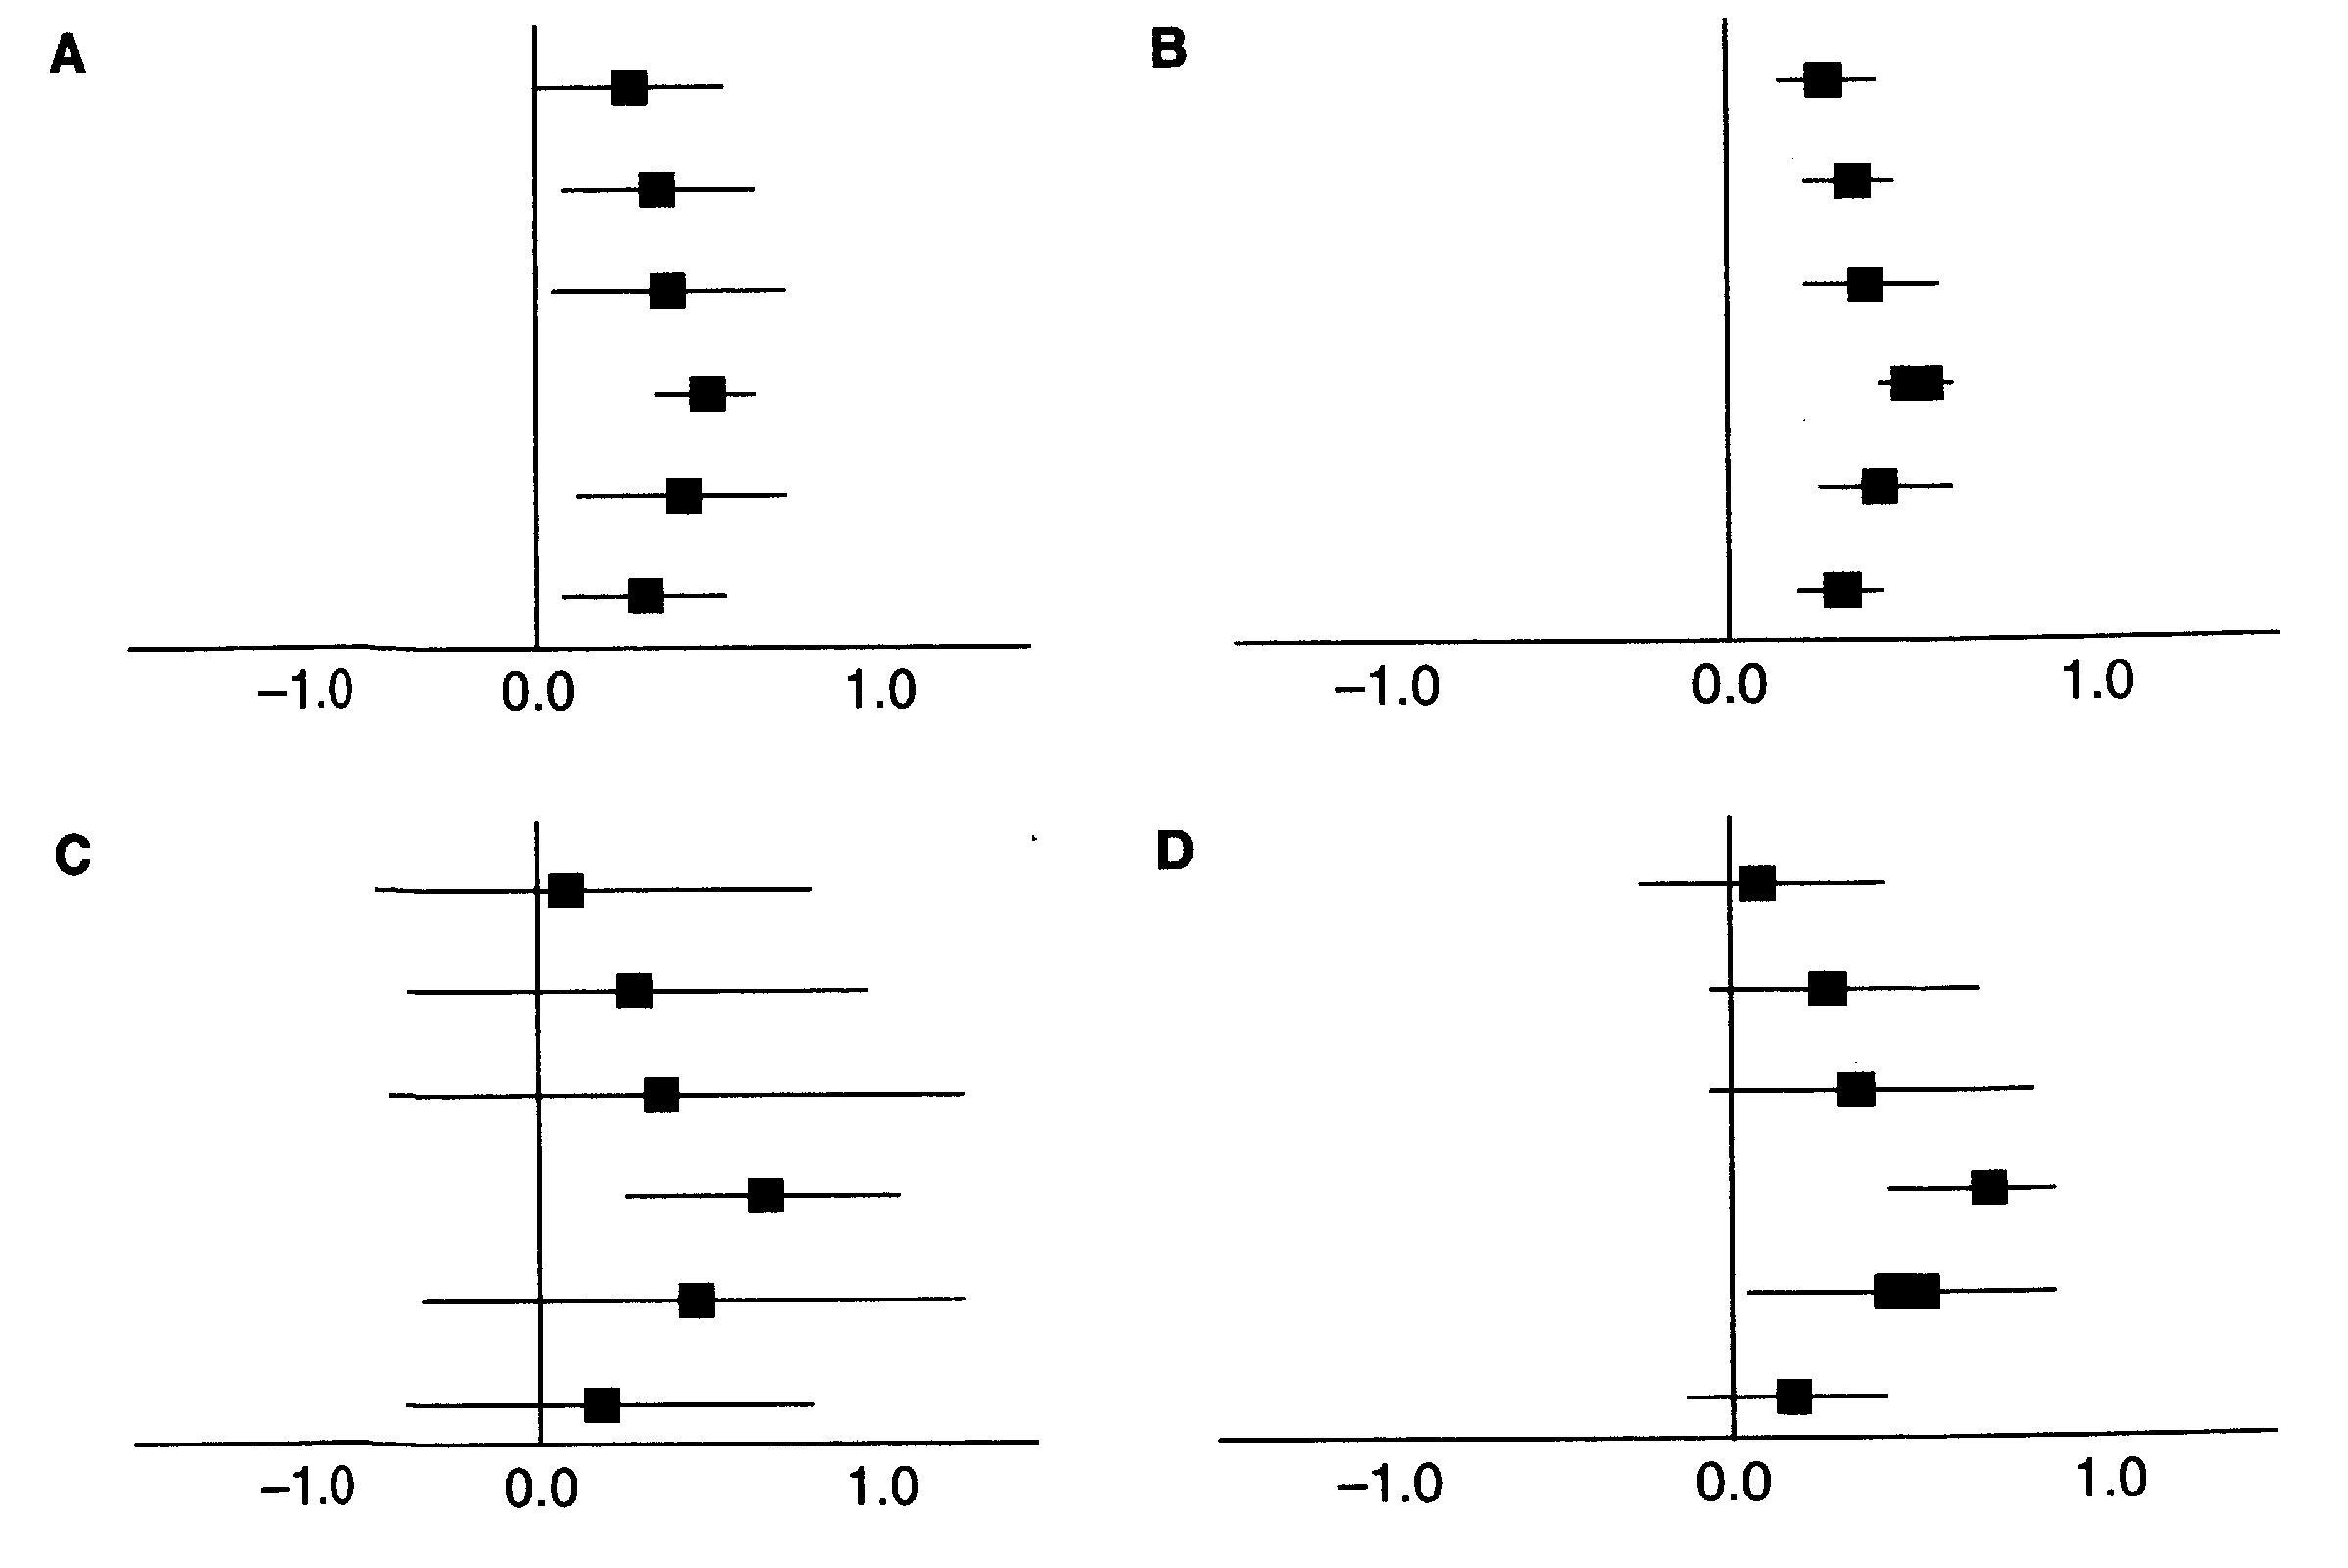
\includegraphics[width=\textwidth]{borenstein108}
\newline(Quelle: Borenstein et al. 2009: 108)
\end{frame}


\begin{frame}[shrink = 5]
  \frametitle{Beispiel für das Verhältnis von Binnen- (within) und Zwischenstudienvarianz (between)}\label{q-werte}
  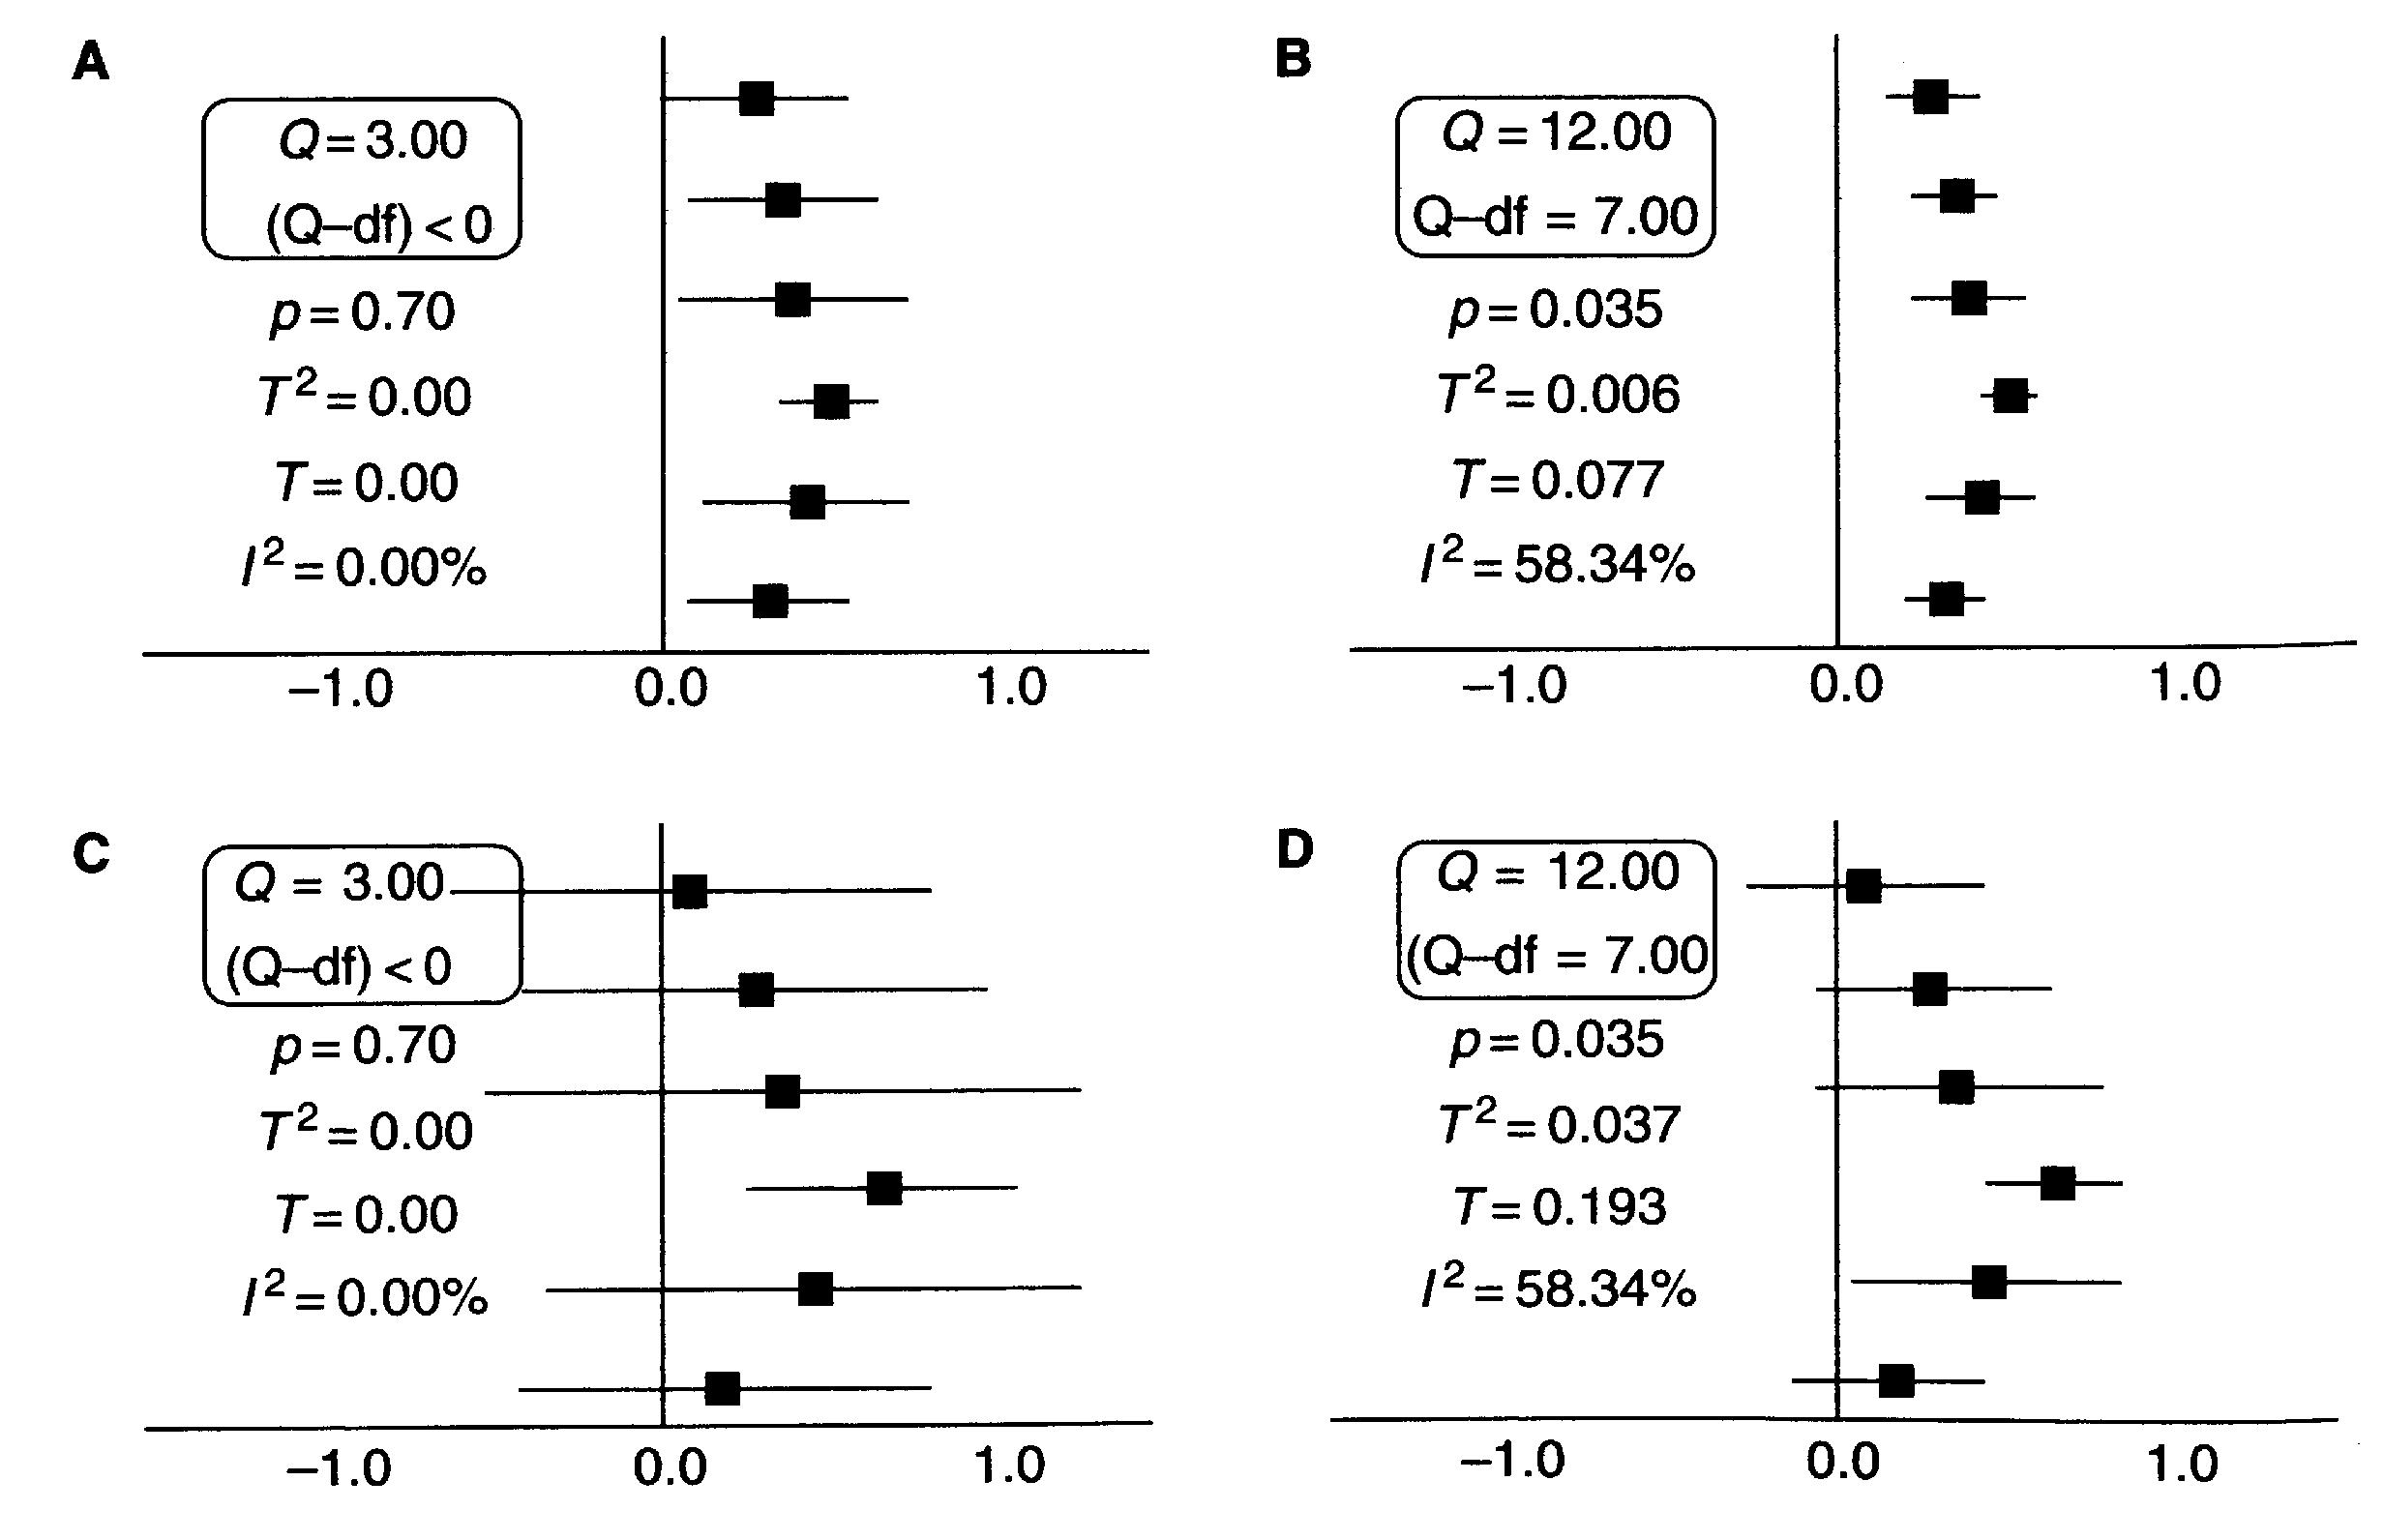
\includegraphics[width=\textwidth]{borenstein110}
\newline(Quelle: Borenstein et al. 2009: 110)
\end{frame}

\newcommand{\lr}{\leftrightarrow}
\begin{frame}[plain]
  \frametitle{Exkurs: Dimensionale Analyse von $Q$ und $\tau^2$}
  %%
  \begin{small}
    \textbf{Ausgangsproblem:} Die Zwischenstudienvarianz ergibt sich nach
    $\tau^2 = \frac {Q-df}{C}$. $C$ wird u.a. benötigt, um die
    Originalmetrik/-dimensionalität wieder herzustellen ("`putting the measure
    back into its original metric"', Borenstein et al. S. 114).

    \textbf{Vorbemerkungen:} Ich werde dimensionale Gleichheit mit dem Zeichen
    $\leftrightarrow$ kennzeichnen und die Dimension in eckigen Klammern
    darstellen, also $[r]$ für einen Korrelationskoeffizienten. Ein leeres
    eckiges Klammerpaar $[\,]$ bezeichnet Dimensionslosigkeit.

    \begin{itemize}
    \item Sei $\tau^2 = \frac {Q-df}{C} \lr [r^2] $ und $w = \frac{1}{SE^2} \lr
      [\frac{1}{r^2}]$.
    \item Für $Q$ und $df$ gilt: $Q = \sum \frac
      {(T_j-\overline{T}_{FEM})^2}{SE_j^2} \lr \sum\frac{[r^2]}{[r^2]} = [\,]$
      und $df=[\,]$ und damit $Q-df \lr [\,]-[\,] = [\,]$.
    \item Für $C$ gilt: $C=\sum w - \frac {\sum w^2}{\sum w} \lr [\frac
      {1}{r^2}] - \frac{[\frac {1}{r^4}]}{[\frac {1}{r^2}]} = [\frac {1}{r^2}] -
      ([\frac {1}{r^4}] \cdot [\frac {r^2}{1}]) = [\frac{1}{r^2}]$.
    \item Daraus folgt für $\tau^2 = \frac{Q-df}{C} \lr
      \frac{[\,]}{[\frac{1}{r^2}]} = [\,]\cdot [r^2] = [r^2]$.
    \end{itemize}
  \end{small}
\end{frame}



\subsection{Weitere Heterogenitätsmaße: $H^2$ und $I^2$}


\begin{frame}
  \frametitle{Kritik an den bisherigen Heterogenitätstests/-statistiken}
  %%
  Probleme mit den bisherigen Heterogenitätsstatistiken:
  \begin{itemize}[<+->]
  \item $\tau^2$ ist nicht zwischen Meta-Analysen vergleichbar; hängt von ES ab.
  \item $Q$ hat geringe statistische Testpower (hoher $\beta$-Fehler).
  \end{itemize}
  \pause
  Eine verbesserte Statistik sollte folgende Kriterien erfüllen:
   \begin{itemize}[<+->]
    \item Abhängigkeit vom Ausmaß der Heterogenität ("`Dependence on the extent of heterogeneity"').
    \item Skaleninvarianz ("`Scale invariance"').
    \item Unabhängigkeit von der Fallzahl $k$ ("`Size invariance"').
  \end{itemize}

\citep[Quelle: ][]{higgins_quantifying_2002}

\end{frame}

\begin{frame}
  \frametitle{$H$}
%
\begin{equation}
  \label{eq:hetero-h-statistic}
  H=\sqrt{\frac{Q}{k-1}}.
\end{equation}
%%
$H$ wird interpretiert als eine an der Zahl der Freiheitsgrade standardisierte $Q$-Statistik.
\end{frame}


\begin{frame}[shrink = 5]
  \frametitle{Konzeptionelle und statistische Definition von $I^2$}
  %%
  \begin{itemize}
  \item $I^2$ ist \emph{konzeptionell} das prozentuale Verhältnis der
    Zwischengruppenvarianz zur Gesamtvarianz (ähnlich wie der ICC für HLM):
    \begin{equation*}
      I^2 = \frac{Zwischenstudienvarianz}{Gesamtvarianz}\times 100 =  \frac{\tau^2}{\tau^2 + \sigma^2}\times 100
    \end{equation*}

  \item Die Maßzahl $I^2$ selbst lässt sich aus $H^2$ ableiten und schätzen:
    %%
    \begin{equation*}
      \label{eq:hetero-i-statistic}
      I^2=\frac{H^2-1}{H^2} \times 100 = \frac{Q-(k-1)}{Q} \times 100 = \frac{Q-df}{Q} \times 100.
    \end{equation*}
  \item Werte von $I^2$ um $25\%$ ($I^2=0,25$) entsprechen einer niedrigen Heterogenität. Dagegen sind Werte um $50\%$
    ($I^2 = $\numprint{0,50}) Anzeichen für eine milde und Werte um $75\%$ Anzeichen für eine deutliche Heterogenität.
  \end{itemize}
\end{frame}



\begin{frame}[shrink = 5]
  \frametitle{Der Zusammenhang zwischen $Q$ und  $I^2$}
  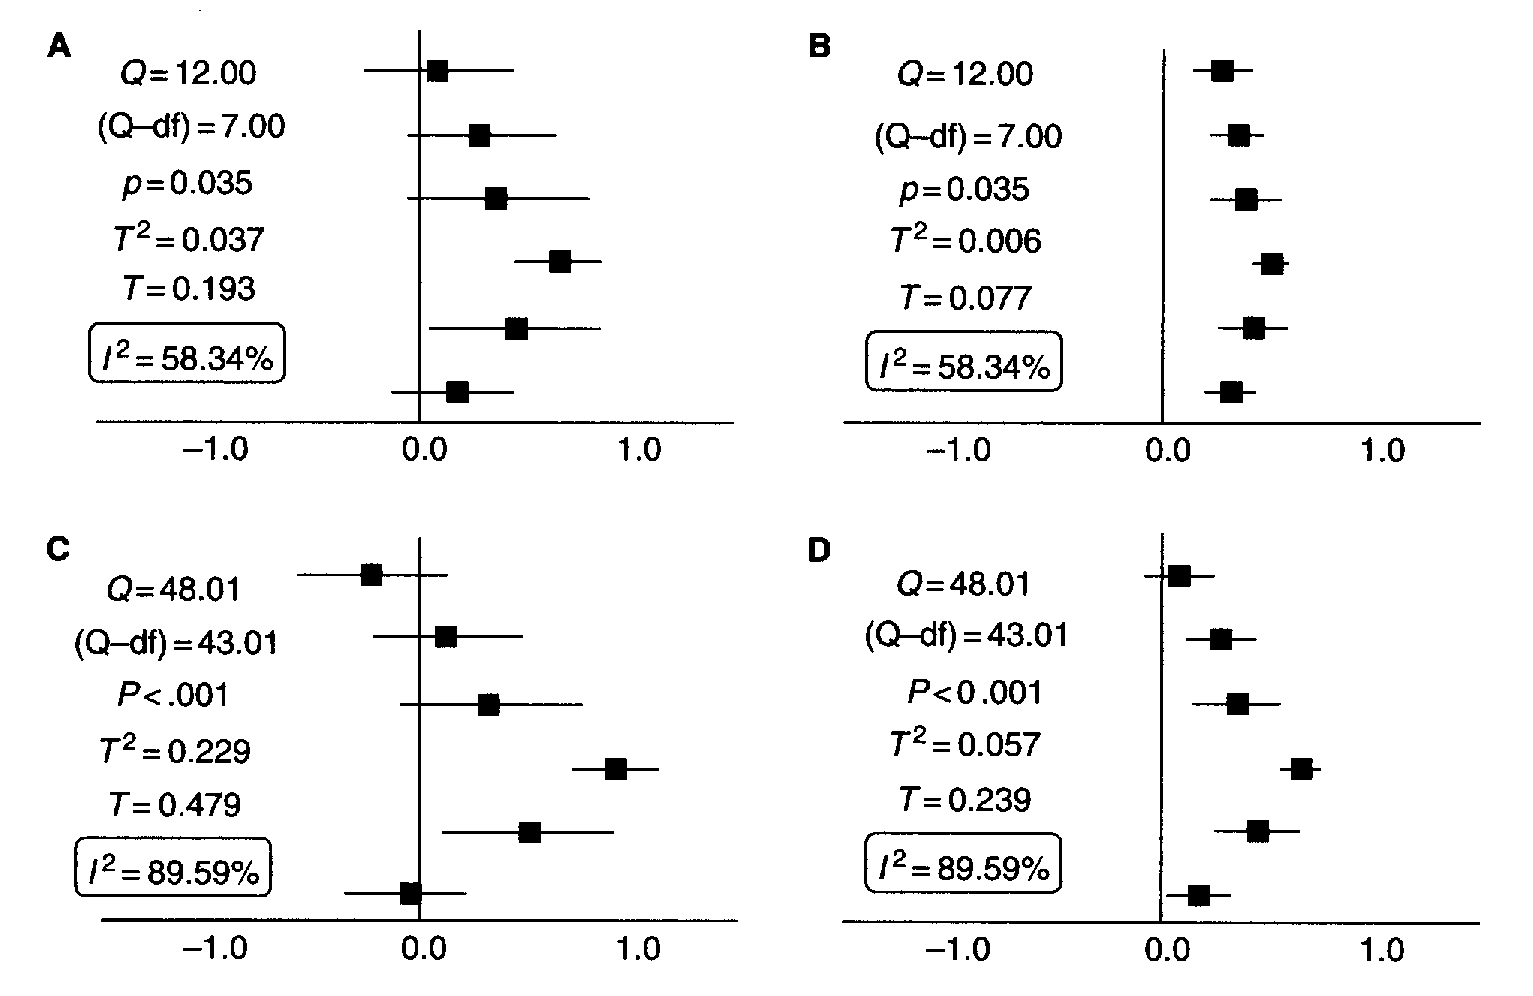
\includegraphics[width=\textwidth]{borenstein118}
  \newline(Quelle: Borenstein et al. 2009: 118)
\end{frame}



\begin{frame}
  \frametitle{Unsicherheits-/Konfidenzintervall (KI) für $I^2$}
  %%
  \begin{itemize}
  \item Das KI für $I^2$ kann nicht direkt berechnet werden, sondern wird über den Standardfehler (SE) von $Q$ bzw. $ln(Q)$ abgeleitet.
  \item Bei der Berechnung des SE von $ln(Q)$ müssen zwei Fälle unterschieden werden: (a) $Q > (df+1)$ und (b) $Q \leq (df+1)$.
  \item Anschließend lässt sich bspw. das $95\%$-KI für $ln(Q)$ \emph{konzeptionell} nach ($Statistik \pm 1,96 \times SE$) berechnen.
  \item Wenn das KI für $I^2$ die 0 einschließt, dann wird von einer \emph{homogenen} Effektstärkenverteilung (FEM)
    ausgegangen.
  \end{itemize}
  (Quelle: Higgins/Thompson 2002: 1554f; Borenstein et al. 2009: 124f)
\end{frame}



\lstset{breaklines=true}


\begin{frame}
  \frametitle{Vergleich zwischen $I^2$ und $Q$}
  \begin{itemize}
  \item "`With respect to the control of Type I error rate, the performance of
    the $Q$ test and the $I^2$ confidence interval was very similar"' (203).
  \item "`With respect to statistical power, there were no notable differences
    between the $Q$ test and the $I^2$ confidence interval"' (203) .
  \item "`In summary, our findings show that the $I^2$ confidence interval
    performs in a similar way to the $Q$ test from an inferential point of
    view"' (204).
  \end{itemize}

\citep[Quelle: ][]{huedo-medina_assessing_2006}

\end{frame}



\subsection{Zusammenfassung Heterogenitätsmaße}

\begin{frame}[shrink = 5]
  \frametitle{Verschiedene Heterogenitätsmaße im Überblick}
  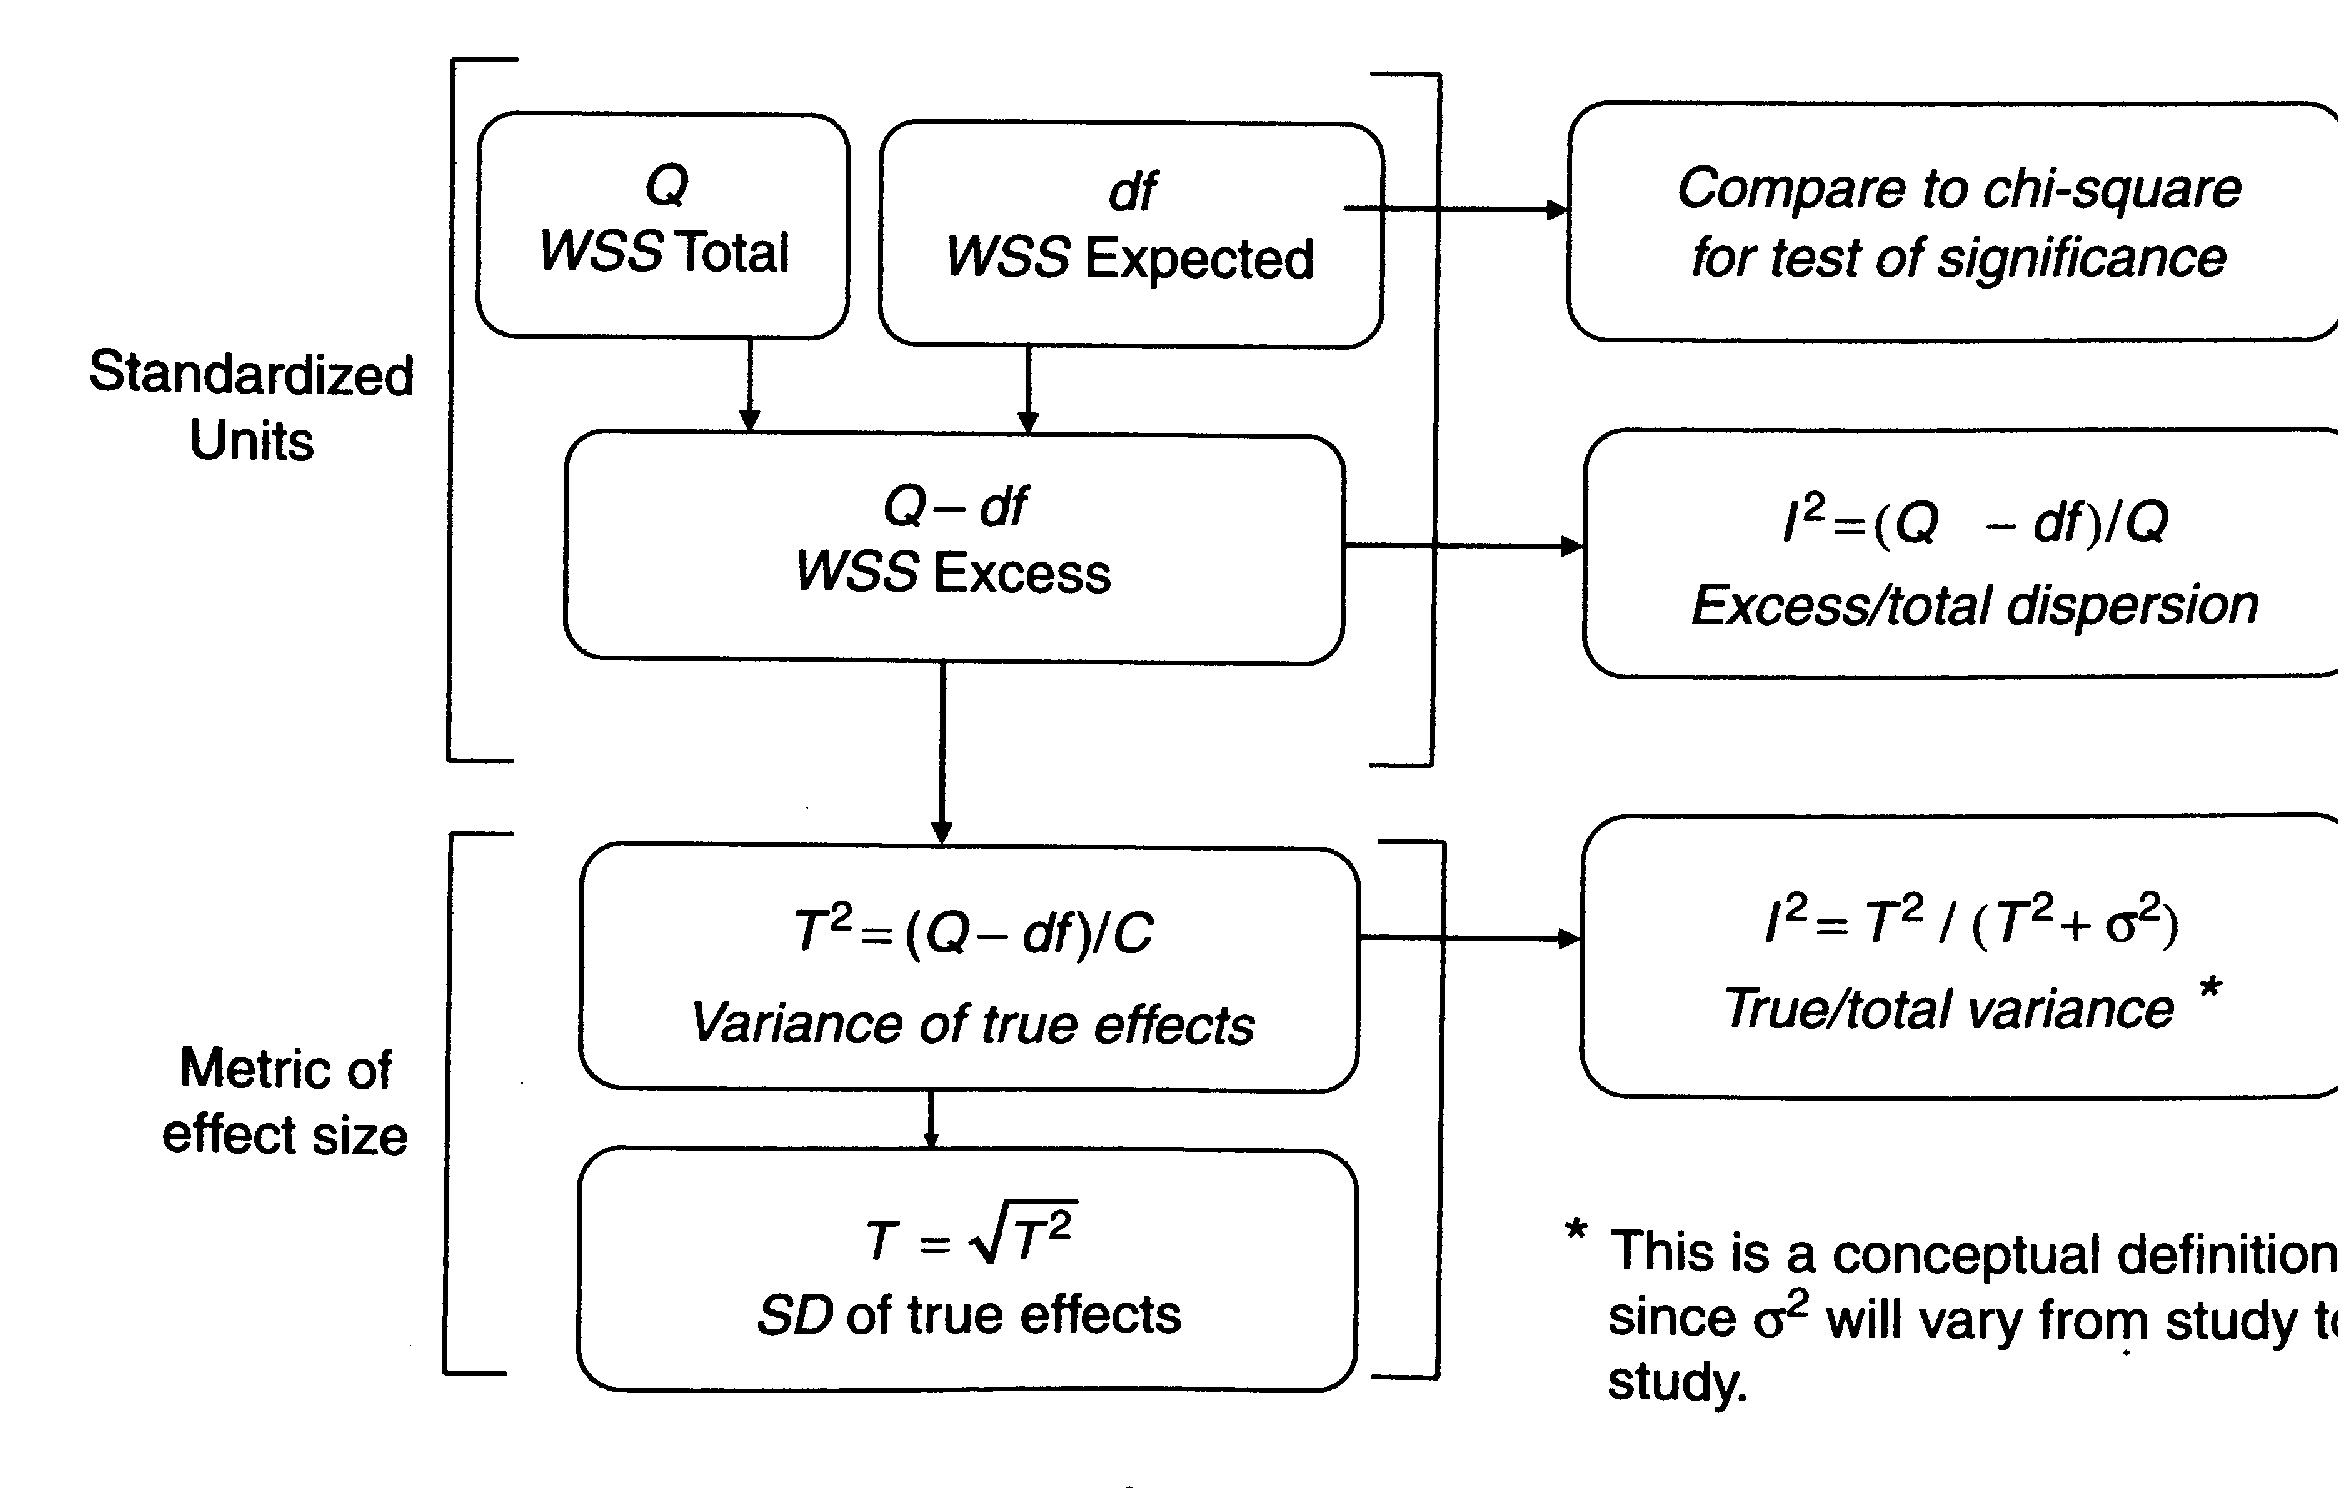
\includegraphics[width=\textwidth]{borenstein111}
\newline(Quelle: Borenstein et al. 2009: 111)
\end{frame}


\begin{frame}
  \frametitle{Zusammenfassende Bemerkungen zur Heterogenität (1)}
  %%
  \begin{itemize}
  \item Im Rahmen einer (aggregatdatenbasierten) Meta-Analyse lassen sich zwei
    Streuungskomponenten unterscheiden:
    \begin{enumerate}
    \item Binnenstudien- (zufallsbedingter Stichprobenfehler; \emph{within};
      $\sigma_j^2$) und
    \item Zwischenstudienvariation (systematische Heterogenität; \emph{between};
      $\tau^2$).
    \end{enumerate}
  \item Die für die ES ($T_j$) unmittelbar beobachtbare Varianz
    $Var(T_j)$ ist \emph{nicht} in der Lage, die Gesamtvariation adäquat zu
    beschreiben (u.a. findet der \emph{within}-Teil keine Berücksichtigung).
  \end{itemize}
\end{frame}


\begin{frame}
  \frametitle{Zusammenfassende Bemerkungen zur Heterogenität (2)}
  %%
  \begin{small}
    Ein sinnvolles Maß zur Beschreibung der Gesamtvariation ist die gewichtete
    Quadratsumme (\emph{weighted sum of squares}) $Q$. Diese muss nun in die
    beiden Streuungskomponenten zerlegt werden:
    \begin{enumerate}
    \item Binnenstudienvariation ($k-1$): Diese Variation der $T_j$ ist allein
      dem Stichprobenfehler geschuldet. Es gibt \emph{keine} Möglichkeit, die
      Binnenstudienvariation in Form einer gemeinsamen (oder gesamten)
      Binnenstudienvarianz auszudrücken. (Allerdings lässt sich für das FEM
      bzw. das REM ein zusammengefasster Standardfehler ($\overline{SE}$)
      bzw. eine Fehlervarianz angeben $\overline{v}$)
    \item Zwischenstudienvariation ($Q-(k-1)$): Es gibt neben dem
      Stichprobenfehler einen (bislang\footnote{Siehe hierzu das Thema
        Meta-Regression.}) unbekannten Einfluss, der zur Variation der $T_j$
      beiträgt. Mit Hilfe der Zwischenstudienvariation lässt sich (ein
      möglicher) Schätzer der Zwischenstudienvarianz ermitteln
      ($\widehat{\tau}^2$).
    \end{enumerate}
  \end{small}
  \end{frame}


\begin{frame}
  \frametitle{Einflussgrößen der Heterogenität (1)}
  %%
  Drei Faktoren haben einen Einfluss auf die Gesamtvariation (sowie ihre beiden Komponenten):
  \begin{enumerate}
  \item der absolute Abstand $|T_j - \overline{T}_{FEM}|$ der $T_j$ zum $\overline{T}_{FEM}$,
  \item der Standardfehler $SE_j$ der einzelnen $T_j$ sowie
  \item die Anzahl ($k$) der $T_j$.
  \end{enumerate}
\end{frame}


\begin{frame}
  \frametitle{Einflussgrößen der Heterogenität (2)}
  %%
  Diese drei Einflussgrößen stehen teilweise in einem entgegengesetzten Verhältnis zu $Q$, $\tau^2$ und
    $I^2$. Werden die anderen beiden Einflussgrößen konstant gehalten, dann führt ein Vergrößern von
    \begin{itemize}
    \item $|T_j - \overline{T}_{FEM}|$ zu einem höheren $Q$ und, sofern $Q-df > 0$ gilt, auch zu einem höheren $\tau^2$
      und $I^2$.
    \item $k$ zu einem höheren $Q$ (da sich auch $Q-df$ ändert, folgt nicht zwangsläufig eine Erhöhung von $\tau^2$
      oder $I^2$).
    \item $SE_j$ zu einem kleineren $Q$ und, sofern noch $Q-df > 0$ gilt, auch zu einem kleineren $\tau^2$ und damit
      auch $I^2$.
    \end{itemize}
 \end{frame}


 \begin{frame}[plain]\frametitle{Interaktives Erforschen der verschiedenen Heterogenitätsmaße}
   %%
   \begin{center}
     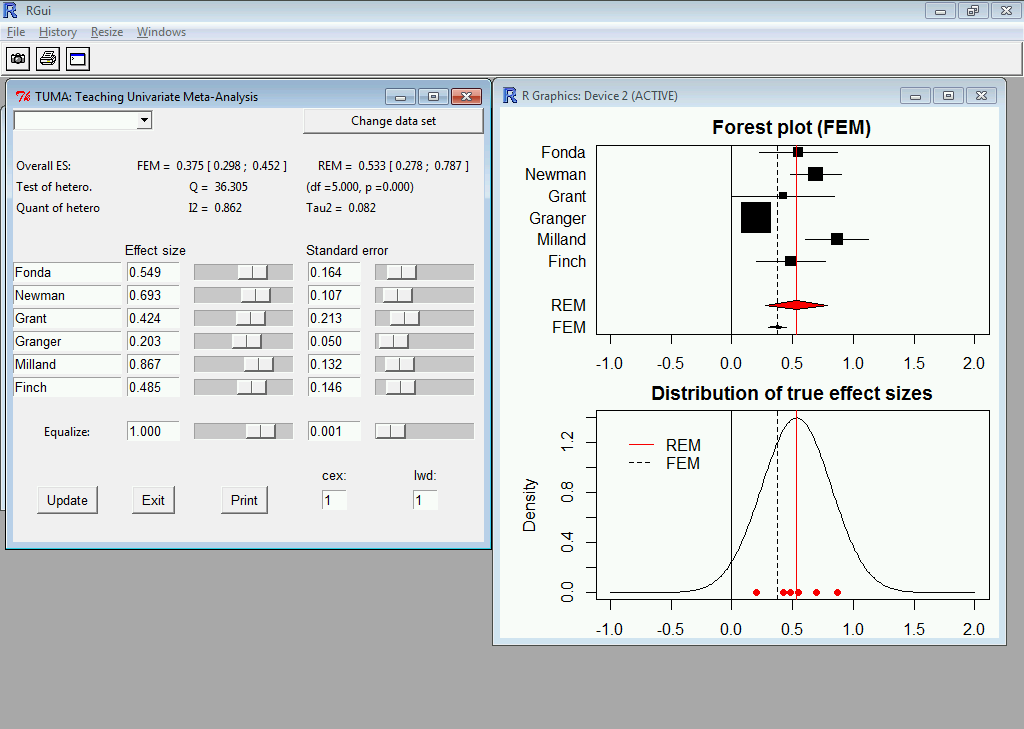
\includegraphics[width=0.8\textwidth]{f_screenshot_tuma.png}
   \end{center}
   (Quelle: \url{https://github.com/berndweiss/tuma})
 \end{frame}


\section{Heterogenitätsaufklärung}

\begin{frame}
  \frametitle{Methoden zur Heterogenitätsaufklärung }
  %%
  Methoden:
  \begin{itemize}
  \item Subgruppenanalysen (vergleichbar ANOVA; fixed-effects oder mixed-effects model)
  \item Meta-Regression (fixed-effects oder mixed-effects model)
  \end{itemize}
  Erklärungsfaktoren (unabh. Variablen, Prädiktoren):
  \begin{itemize}
  \item (Aggregierte) Individualmerkmale (Achtung: Gefahr eines ökologischen Fehlschlusses, siehe Folie \pageref{ref:oekofehlschluss})
  \item Studienmerkmale
  \end{itemize}
  Abhängige Variable: Effektstärken (Zusammenhangsmaße; damit wird ein Interaktionseffekt modelliert)
\end{frame}


\subsection{Meta-Regression}


\begin{frame}
  \frametitle{Was ist eine Meta-Regression?}

  "`We use the term meta-regression to indicate the use of trial-level covariates, as distinct from regressionan analyses
  that are possible when individual patient data on outcomes and covariates are available"' \citep[1560]{thompson_how_2002}.

\end{frame}


\begin{frame}
  \frametitle{Das FEM der Meta-Regression}
  %%
  \begin{itemize}
  \item Ohne Kovariaten (= Nullmodell) bestimmt sich der Schätzer des FEM nach:
    $T_j = \theta + \epsilon_j$ und es wird angenommen, dass $T_j \sim N(\theta,
    \sigma_j^2)$ für $j = 1,2,\ldots,k$ Studien.
  \item Für $X_1, \ldots, X_p$ Prädiktorvariablen (Kovariaten,
    unabh. Variablen) bestimmt sich das FE Regressionsmodell nach:
    \begin{equation}\label{eq:fem-reg}
      \theta_j = \theta = \beta_0 + \beta_1 x_1 + \ldots + \beta_px_p
    \end{equation}
  \item Gleichung \ref{eq:fem-reg} lässt sich auflösen nach:
    \begin{equation}
      T_j = \beta_0 + \beta_1 x_1 + \ldots + \beta_px_p + \epsilon_j
    \end{equation}
  \end{itemize}

  \citep[Quelle: ][94]{sutton_methods_2000}

\end{frame}


\begin{frame}[plain]
  \frametitle{Das FEM der Meta-Regression: Vorgehen}
  %%
  \begin{itemize}
  \item Das (lineare) FEM der Meta-Regression wird nicht mit Hilfe eines OLS-
    (\emph{ordinary least squares}), sondern eines WLS-Schätzers (\emph{weighted
      least squares}) ermittelt.
  \item Als Gewichte wird die inverse Fehlervarianz verwendet, also $w_j =
    \frac{1}{SE_j^2}$.
  \item Eine WLS-Regression lässt sich mit den meisten Statistikpaketen
    durchführen, wichtig ist jedoch die anschließende Korrektur der
    Standardfehler (SE) der Regressionskoeffizienten ($\beta_j$) nach
    \begin{equation}
      SE^{korrigiert}_j = \frac{SE^{original}_j}{\sqrt{MS_{error}}}.
    \end{equation}
  \item Die Gesamtvariation ($Q$) lässt sich in zwei Komponenten zerlegen, in
    $Q_{resid}$ ($df=k-p-1$) (oder $Q_{error}$, unerklärte Variation) und
    $Q_{model}$ ($df=p$) (erklärte Variation).
  \end{itemize}
\end{frame}


\begin{frame}[shrink = 5]
  \frametitle{Das FEM der Meta-Regression}
  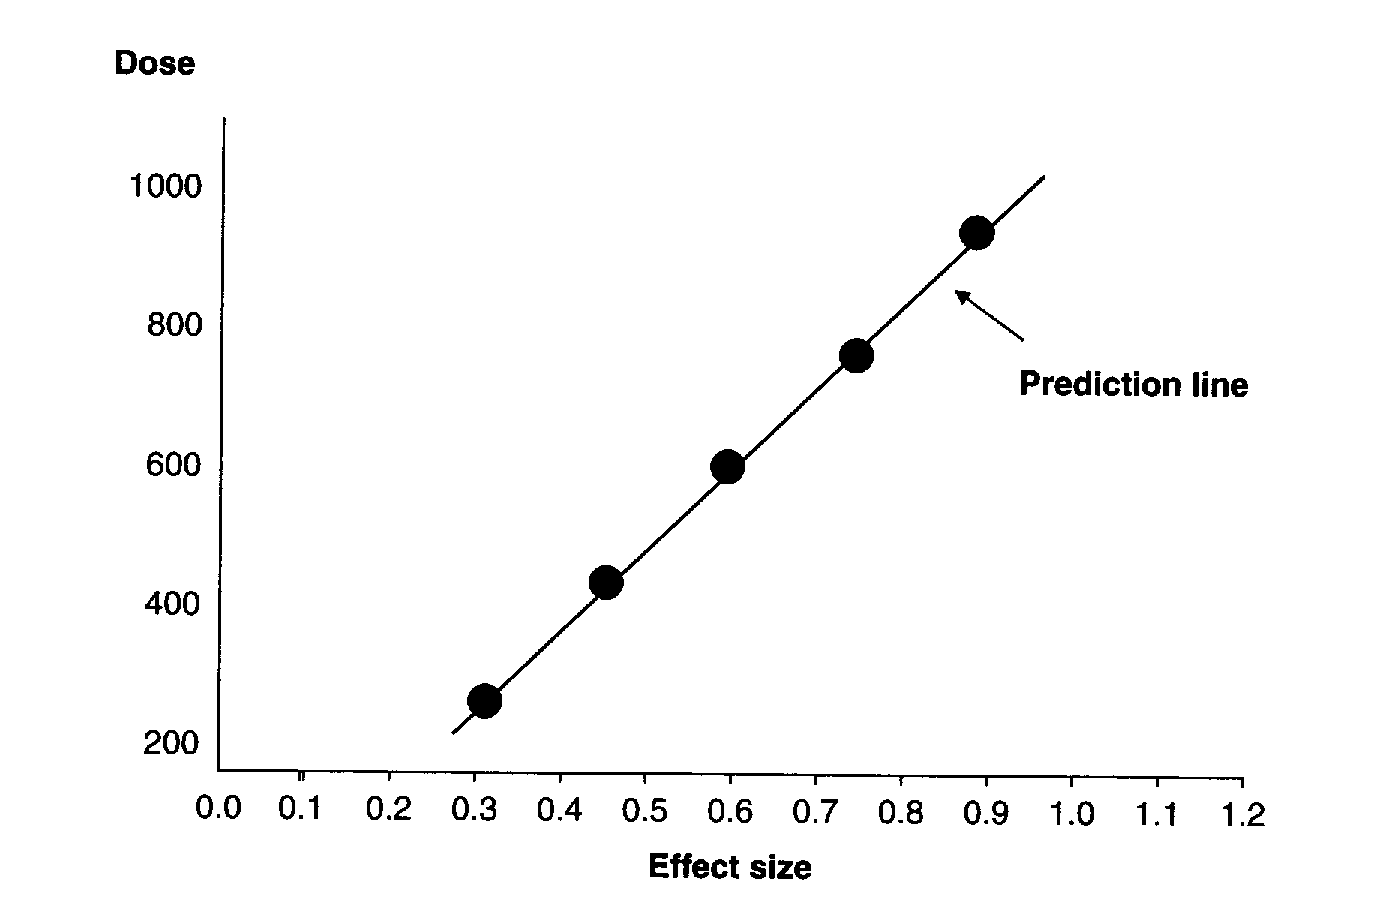
\includegraphics[width=\textwidth]{borenstein194a}
\newline(Quelle: Borenstein et al. 2009: 194)
\end{frame}



\begin{frame}[plain]
  \frametitle{"`Mixed-effects"' Regression (das "`REM"' der Meta-Regression)}
  %%
  \begin{itemize}
  \item Ohne Kovariaten (= Nullmodell) bestimmt sich der Schätzer des REM nach:
    $T_j = \theta_j + \epsilon_j = \theta + \epsilon_j + u_j$ und es wird angenommen, dass
    $\theta_j \sim N(\theta, \tau^2)$ für $j = 1,2,\ldots,k$.
  \item Für $X_1, \ldots, X_p$ Prädiktorvariablen (Kovariaten, unabh. Variablen)
    ergibt sich das \emph{mixed-effects model} nach:
    \begin{equation}
      T_j = \beta_0 + \beta_1 x_1 + \ldots + \beta_px_p + \epsilon_j + u_j.
    \end{equation}
  \item Im Fall von erklärungskräftigen Prädiktoren reduziert sich $\tau^2$ und
    es lässt sich der Anteil an erklärter Zwischenstudienvarianz berechnen: $R^2
    = 1- \frac{\tau^2_{unerklaert}}{\tau^2_{Gesamt/Nullmodell}}$.
  \end{itemize}

  \citep[Quelle: ][98]{sutton_methods_2000}
\end{frame}


\begin{frame}[shrink = 5]
  \frametitle{Das "`REM"' der Meta-Regression}
  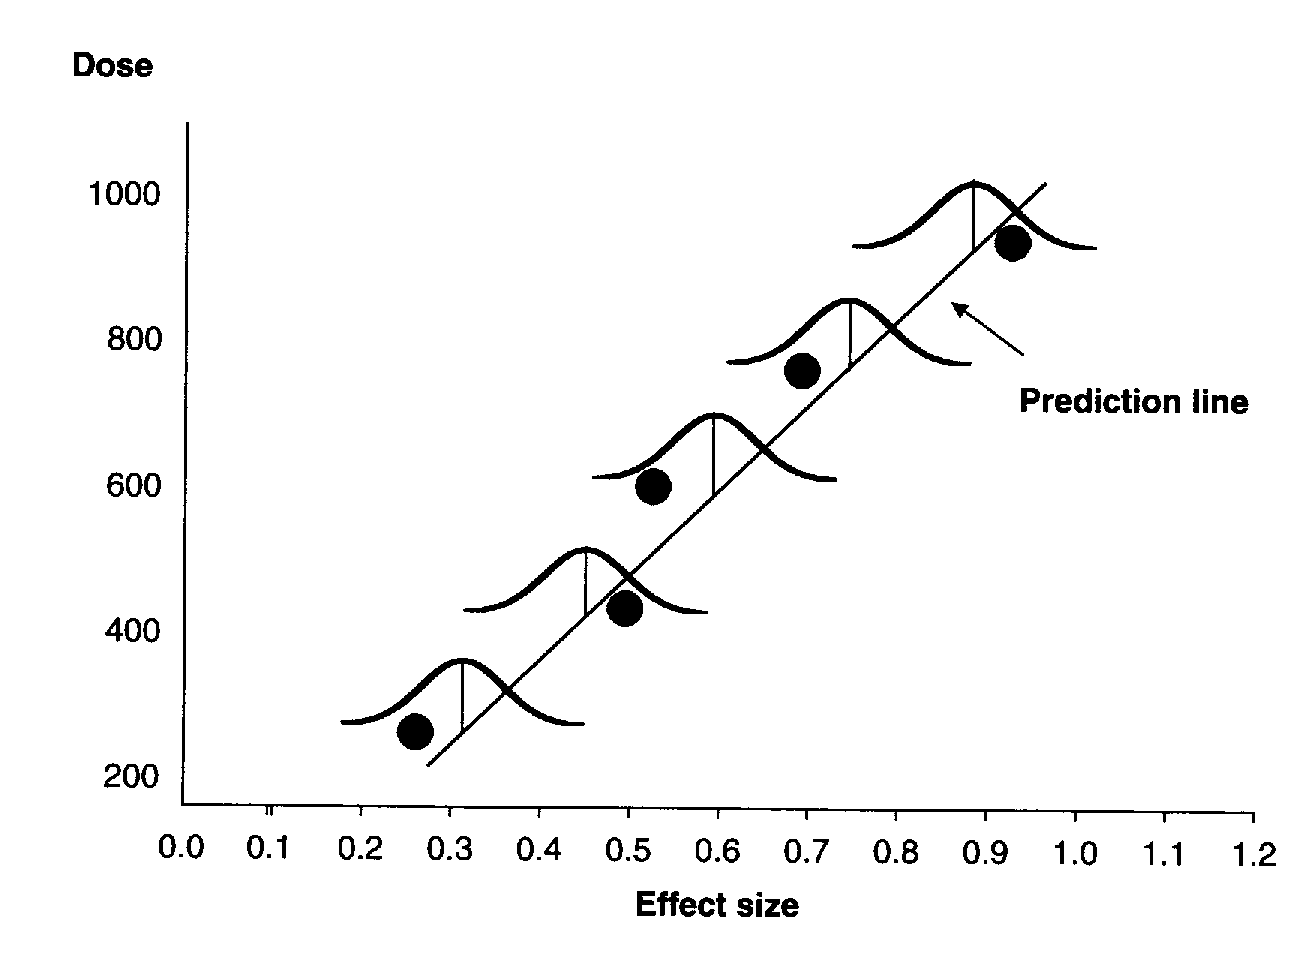
\includegraphics[width=\textwidth]{borenstein194b}
\newline(Quelle: Borenstein et al. 2009: 194)
\end{frame}


\begin{frame}
  \frametitle{Beispiel: Wirksamkeit des BCG-Impfstoffs zur Bekämpfung der Tuberkulose}
  \framesubtitle{Fragestellung}

  \begin{itemize}
  \item Es gibt zahlreiche (13) Studien, welche die Wirksamkeit des
    BCG-Impfstoff zur Verhinderung der Tuberkulose untersuchen.
  \item Kontrollgruppe sind ungeimpfte Personen, als Effektstärke wird das
    \emph{relative risk} (RR) verwendet. Beispiel:
    \begin{itemize}
    \item Geimpft: 4 erkrankt, 119 nicht erkrankt
    \item Nicht geimpft: 11 erkrankt, 128 nicht erkrankt
    \item RR: (4/(4+119))/(11/(11+128)) = 0.4109
    \end{itemize}
  \item Es wird vermutet, dass der Impfstoff in kälteren Klimazonen wirksamer
    ist und daher das RR mit der Entfernung zum Äquator (hier: geographische
    Breite) zunimmt.
  \end{itemize}
\end{frame}





\begin{frame}[fragile, plain]
  \frametitle{Beispiel: Wirksamkeit des BCG-Impfstoffs zur Bekämpfung der
    Tuberkulose} \framesubtitle{Datensatz}

  \begin{footnotesize}
\begin{knitrout}
\definecolor{shadecolor}{rgb}{0.827, 0.827, 0.827}\color{fgcolor}\begin{kframe}
\begin{verbatim}
   tpos  tneg cpos  cneg ablat       yi       vi
1     4   119   11   128    44 -0.88931 0.325585
2     6   300   29   274    55 -1.58539 0.194581
3     3   228   11   209    42 -1.34807 0.415368
4    62 13536  248 12619    52 -1.44155 0.020010
5    33  5036   47  5761    13 -0.21755 0.051210
6   180  1361  372  1079    44 -0.78612 0.006906
7     8  2537   10   619    19 -1.62090 0.223017
8   505 87886  499 87892    13  0.01195 0.003962
9    29  7470   45  7232    27 -0.46942 0.056434
10   17  1699   65  1600    42 -1.37134 0.073025
11  186 50448  141 27197    18 -0.33936 0.012412
12    5  2493    3  2338    33  0.44591 0.532506
13   27 16886   29 17825    33 -0.01731 0.071405
\end{verbatim}
\end{kframe}
\end{knitrout}


tpos = treatment group, erkrankt; tneg = treatment group, nicht erkrankt; cpos =
control group, erkrankt; cneg = control group, nicht erkrankt; ablat =
Abs. Breitengrad
  \end{footnotesize}
\end{frame}



\begin{frame}[fragile]
  \frametitle{Beispiel: Wirksamkeit des BCG-Impfstoffs zur Bekämpfung der
    Tuberkulose} \framesubtitle{Nullmodel}

\begin{tiny}
\begin{knitrout}
\definecolor{shadecolor}{rgb}{0.827, 0.827, 0.827}\color{fgcolor}\begin{kframe}
\begin{verbatim}

Random-Effects Model (k = 13; tau^2 estimator: DL)

tau^2 (estimate of total amount of heterogeneity): 0.3088
tau (sqrt of the estimate of total heterogeneity): 0.5557
I^2 (% of total variability due to heterogeneity): 92.12%
H^2 (total variability / sampling variability):    12.69

Test for Heterogeneity: 
Q(df = 12) = 152.2330, p-val < .0001

Model Results:

estimate       se     zval     pval    ci.lb    ci.ub          
 -0.7141   0.1787  -3.9952   <.0001  -1.0644  -0.3638      *** 

---
Signif. codes:  0 '***' 0.001 '**' 0.01 '*' 0.05 '.' 0.1 ' ' 1 
\end{verbatim}
\end{kframe}
\end{knitrout}

\end{tiny}
\end{frame}


\begin{frame}[fragile]
  \frametitle{Beispiel: Wirksamkeit des BCG-Impfstoffs zur Bekämpfung der
    Tuberkulose} \framesubtitle{Fixed-effects model}

\begin{tiny}
\begin{knitrout}
\definecolor{shadecolor}{rgb}{0.827, 0.827, 0.827}\color{fgcolor}\begin{kframe}
\begin{verbatim}

Fixed-Effects with Moderators Model (k = 13)

Test for Residual Heterogeneity: 
QE(df = 11) = 30.7331, p-val = 0.0012

Test of Moderators (coefficient(s) 2): 
QM(df = 1) = 121.4999, p-val < .0001

Model Results:

         estimate      se      zval    pval    ci.lb    ci.ub     
intrcpt    0.3436  0.0810    4.2390  <.0001   0.1847   0.5024  ***
ablat     -0.0292  0.0027  -11.0227  <.0001  -0.0344  -0.0240  ***

---
Signif. codes:  0 '***' 0.001 '**' 0.01 '*' 0.05 '.' 0.1 ' ' 1 
\end{verbatim}
\end{kframe}
\end{knitrout}

\end{tiny}
\end{frame}



\begin{frame}[fragile]
  \frametitle{Beispiel: Wirksamkeit des BCG-Impfstoffs zur Bekämpfung der Tuberkulose}
  \framesubtitle{Mixed-effects model ("`method of moments"')}

\begin{tiny}
\begin{knitrout}
\definecolor{shadecolor}{rgb}{0.827, 0.827, 0.827}\color{fgcolor}\begin{kframe}
\begin{verbatim}

Mixed-Effects Model (k = 13; tau^2 estimator: DL)

tau^2 (estimate of residual amount of heterogeneity): 0.0633
tau (sqrt of the estimate of residual heterogeneity): 0.2516

Test for Residual Heterogeneity: 
QE(df = 11) = 30.7331, p-val = 0.0012

Test of Moderators (coefficient(s) 2): 
QM(df = 1) = 18.8452, p-val < .0001

Model Results:

         estimate      se     zval    pval    ci.lb    ci.ub     
intrcpt    0.2595  0.2323   1.1172  0.2639  -0.1958   0.7149     
ablat     -0.0292  0.0067  -4.3411  <.0001  -0.0424  -0.0160  ***

---
Signif. codes:  0 '***' 0.001 '**' 0.01 '*' 0.05 '.' 0.1 ' ' 1 
\end{verbatim}
\end{kframe}
\end{knitrout}

\end{tiny}
\end{frame}


\begin{frame}[fragile]
  \frametitle{Beispiel: Wirksamkeit des BCG-Impfstoffs zur Bekämpfung der Tuberkulose}
  \framesubtitle{Mixed-effects model (REML)}

\begin{tiny}
\begin{knitrout}
\definecolor{shadecolor}{rgb}{0.827, 0.827, 0.827}\color{fgcolor}\begin{kframe}
\begin{verbatim}

Mixed-Effects Model (k = 13; tau^2 estimator: REML)

tau^2 (estimate of residual amount of heterogeneity): 0.0764 (SE = 0.0591)
tau (sqrt of the estimate of residual heterogeneity): 0.2763

Test for Residual Heterogeneity: 
QE(df = 11) = 30.7331, p-val = 0.0012

Test of Moderators (coefficient(s) 2): 
QM(df = 1) = 16.3571, p-val < .0001

Model Results:

         estimate      se     zval    pval    ci.lb    ci.ub     
intrcpt    0.2515  0.2491   1.0095  0.3127  -0.2368   0.7397     
ablat     -0.0291  0.0072  -4.0444  <.0001  -0.0432  -0.0150  ***

---
Signif. codes:  0 '***' 0.001 '**' 0.01 '*' 0.05 '.' 0.1 ' ' 1 
\end{verbatim}
\end{kframe}
\end{knitrout}

\end{tiny}
\end{frame}


\begin{frame}[shrink = 5]
  \frametitle{Das "`REM"' der Meta-Regression: Erklärte Varianz}

  \begin{equation}
    R^2 = 1-\frac{\widehat{\tau}_{unexplained}}{\widehat{\tau}_{total}} =
    1-\frac{0.0633}{0.3088} =
    0.795
  \end{equation}

  (Basiert auf den Ergebnissen des MM-Schätzer.)

  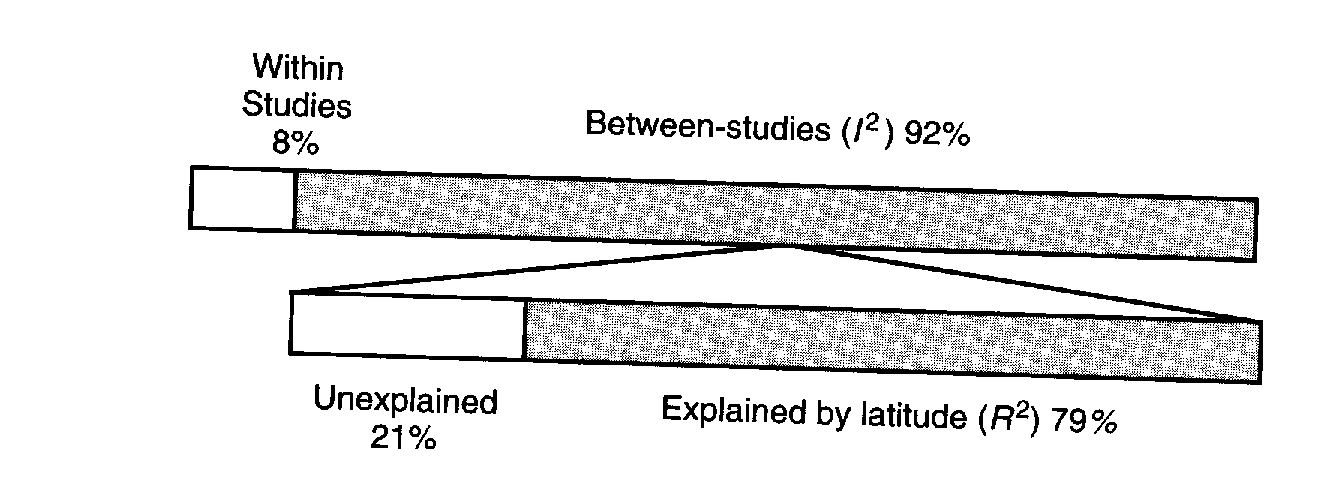
\includegraphics[width=\textwidth]{borenstein202}
\newline(Quelle: Borenstein et al. 2009: 202)

\end{frame}




\subsection{ANOVA-ähnliche Verfahren}


\begin{frame}[plain, shrink]\frametitle{ANOVA-ähnliche Modelle}\framesubtitle{Grundprinzip}
  \begin{itemize}
  \item Die $T_{ji}$ lassen sich ($p$) Gruppen zuweisen, mit $j = 1, \ldots,
    p$ Gruppen, $i = 1, \ldots, k_j$ Studien und $k=\sum k_j$.
  \item Sei weiterhin $T_{j\bullet}$ der geschätzte mittlere Effekt in Gruppe
    $j$ und $\theta_{j\bullet}$ der Parameter für Gruppe $j$, dann
    lautet die erste Frage in einer ANOVA: Unterscheiden sich die
    $\theta_{j\bullet}$ voneinander? Die $H_0$ lautet: $H_0: \theta_{1\bullet} =
    \theta_{2\bullet}=\ldots= \theta_{p\bullet}$.
  \item Die zweite Frage lautet: Unterscheiden sich die $\theta_{ji}$ in der
    $j$-ten Gruppe? Die entsprechende $H_{0j}$ für Gruppe $j$ lautet: $\theta_{j1} = \theta_{j2} = \ldots =
    \theta_{jk_j} = \theta_{j\bullet}$.
  \item Es lassen sich verschiedene Q-Tests durchführen,
    um die "`between"'- und die "`within"'-Variation zu testen. Ist der
    kat. Prädiktor bedeutsam, dann erwarten wir die Zurückweisung von $H_0: \theta_{1\bullet} =
    \theta_{2\bullet}=\ldots= \theta_{p\bullet}$ ("`between-studies variation"'), nicht aber von $H_{0j}: \theta_{j1} = \theta_{j2} = \ldots =
    \theta_{jk_j} = \theta_{j\bullet}$ ("`within variation"').
  \end{itemize}

  \citep[Quelle: Notation vertauscht, $i$ = Studiensubskript][]{becker_edf_2010}

\end{frame}



\begin{frame}
  \frametitle{ANOVA-ähnliche Verfahren}\framesubtitle{Variationszerlegung}
  %%
  \begin{itemize}
  \item Die "`Variationszerlegung"' in  $Q_{within}$, $Q_{between}$ und $Q_{total}$ folgt der aus der Varianzanalyse
    bekannten Zerlegung in "`sum of squares within/resid"' (SSW), "`sum of squares between/model"' (SSB) and "`sum of
    squares total"' (SST = SSW+SSB). Allerdings werden hier gewichtete Quadratsummen verwendet.
  \item $Q_{total}$: Gesamtvariation; entspricht dem bekannten $Q$ für alle $k$ Studien (Nullmodel; ohne Prädiktoren)
  ($df = k-1$) und es gilt: $Q_{total} = Q_{between} + Q_{within}$.
\item $Q_{within/resid}$: Nicht durch das Modell erklärte Variation ($df = k-p$; $p$ = Anzahl der zu schätzenden Parameter)
\item $Q_{between/model}$: Durch das Modell erklärte Variation ($df = p-1$)
\end{itemize}
\end{frame}


\begin{frame}\frametitle{ANOVA-ähnliche Verfahren}\framesubtitle{Modellwahl: FEM oder REM}
  \begin{itemize}
  \item Wird das FEM angenommen, dann gilt, dass allen Studien in Subgruppe A
    bzw. B. jeweils eine eigene \emph{gemeinsame} ES zugrundeliegt.
  \item Gibt es auch nach Einbeziehung des kategorialen Prädiktors eine
    stat. signifikante \enquote{within}-Variation, dann ist das REM
    angemessen. Wie aber wird die Zwischenstudienvarianz geschätzt?
    \begin{itemize}
    \item Pro Subgruppe ein eigener Schätzer von $\widehat{\tau}^2$ (wird im
      Bsp. auf Folie \pageref{slide:anova-example} angenommen)
    \item Ein über alle Subgruppen \enquote{gepoolter} Schätzer von $\widehat{\tau}^2$
    \end{itemize}
  \end{itemize}
\end{frame}


\begin{frame}\frametitle{Flowchart zur Wahl FEM oder REM}
  \begin{center}
    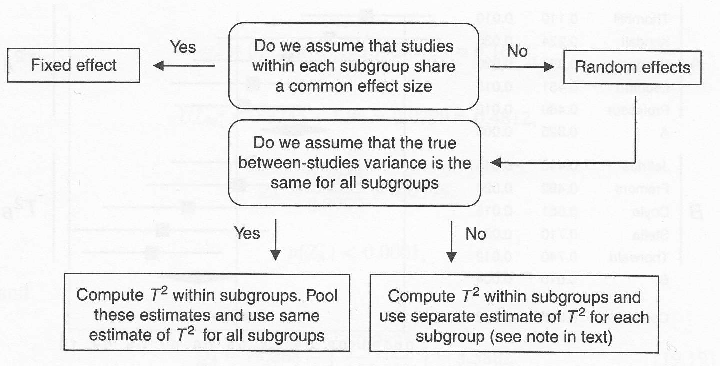
\includegraphics[width=\textwidth]{f_borenstein_163.pdf}
  \end{center}
  \citep[Quelle:][163]{borenstein_introduction_2009}
\end{frame}


\begin{frame}[fragile]
  \frametitle{Beispiel für meta-analytische Subgruppenanalyse}
  \framesubtitle{Datensatz}

\begin{knitrout}
\definecolor{shadecolor}{rgb}{0.827, 0.827, 0.827}\color{fgcolor}\begin{kframe}
\begin{verbatim}
       y     V g     SE
1  0.110 0.010 A 0.1000
2  0.224 0.030 A 0.1732
3  0.338 0.020 A 0.1414
4  0.451 0.015 A 0.1225
5  0.480 0.010 A 0.1000
6  0.440 0.015 B 0.1225
7  0.492 0.020 B 0.1414
8  0.651 0.015 B 0.1225
9  0.710 0.025 B 0.1581
10 0.740 0.012 B 0.1095
\end{verbatim}
\end{kframe}
\end{knitrout}

y = Hedges' g, V=Varianz, g=Gruppe, SE=Standardfehler\\
\citep[Quelle: ][152]{borenstein_introduction_2009}

\end{frame}


\begin{frame}[fragile, plain, shrink=10]
  \frametitle{Beispiel für meta-analytische Subgruppenanalyse}\label{slide:anova-example}
\begin{tiny}
\begin{knitrout}
\definecolor{shadecolor}{rgb}{0.827, 0.827, 0.827}\color{fgcolor}\begin{kframe}
\begin{verbatim}
                     95%-CI %W(fixed) %W(random)
1  0.110  [-0.0860; 0.3060]     15.23      11.61
2  0.224  [-0.1155; 0.5635]      5.08       7.74
3  0.338  [ 0.0608; 0.6152]      7.61       9.29
4  0.451  [ 0.2110; 0.6910]     10.15      10.32
5  0.480  [ 0.2840; 0.6760]     15.23      11.61
6  0.440  [ 0.2000; 0.6800]     10.15      10.32
7  0.492  [ 0.2148; 0.7692]      7.61       9.29
8  0.651  [ 0.4110; 0.8910]     10.15      10.32
9  0.710  [ 0.4001; 1.0199]      6.09       8.44
10 0.740  [ 0.5253; 0.9547]     12.69      11.06

Number of studies combined: k=10

                                       95%-CI      z  p.value
Fixed effect model   0.4581  [0.3816; 0.5346] 11.740 < 0.0001
Random effects model 0.4638  [0.3305; 0.5972]  6.816 < 0.0001

Quantifying heterogeneity:
tau^2 = 0.0299; H = 1.71 [1.23; 2.4]; I^2 = 66% [33.4%; 82.6%]

Test of heterogeneity:
     Q d.f.  p.value
 26.44    9   0.0017

Results for subgroups (fixed effect model):
        k                   95%-CI    Q    tau^2   I^2
g = A   5 0.3241  [0.2193; 0.4289] 8.43   0.0164 52.6%
g = B   5 0.6111  [0.4992; 0.7230] 4.54   0.0022   12%

Test for subgroup differences (fixed effect model):
                   Q d.f.  p.value
Between groups 13.46    1   0.0002
Within groups  12.97    8   0.1129

Results for subgroups (random effects model):
        k                   95%-CI    Q    tau^2   I^2
g = A   5 0.3245  [0.1678; 0.4812] 8.43   0.0164 52.6%
g = B   5 0.6100  [0.4903; 0.7298] 4.54   0.0022   12%

Test for subgroup differences (random effects model):
                    Q d.f.  p.value
Between groups   8.05    1   0.0045

Details on meta-analytical method:
- Inverse variance method
- DerSimonian-Laird estimator for tau^2
\end{verbatim}
\end{kframe}
\end{knitrout}

\end{tiny}
\end{frame}



\begin{frame}[plain]\frametitle{{Publikationsbeispiel für meta-analytische Subgruppenanalyse}}
  \begin{center}
    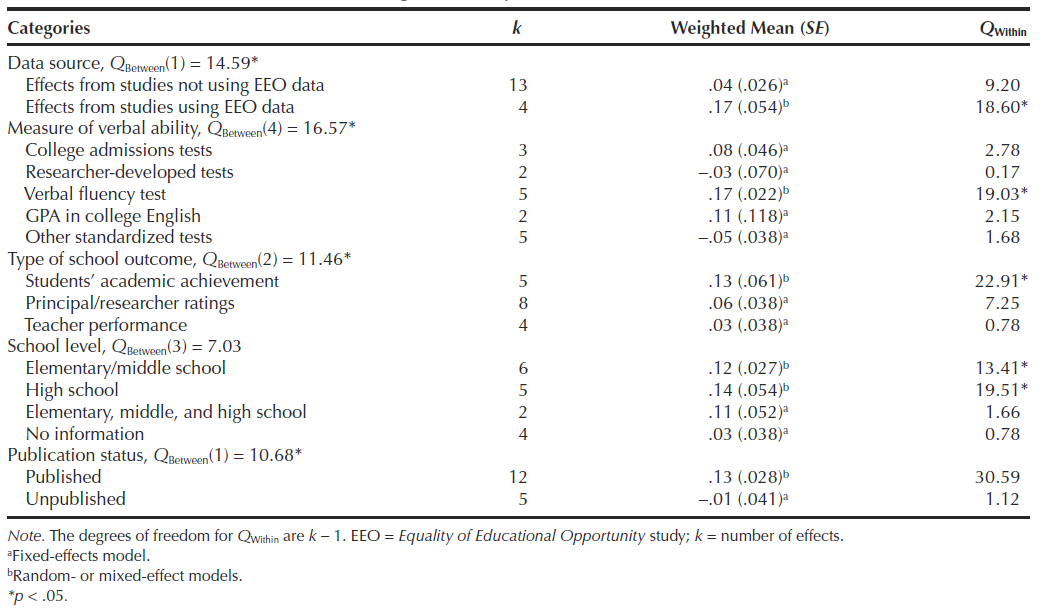
\includegraphics[width=\textwidth]{f_aloe_becker_2009.png}
  \end{center}
  \citep[Quelle:][618]{aloe_teacher_2009}
\end{frame}



\subsection{Weitere Bemerkungen zu Verfahren der Heterogenitätsaufklärung}


\begin{frame}
  \frametitle{Ökologischer Fehlschluss}\label{ref:oekofehlschluss}
  %%
  "`Caution is required, however, because aggregation bias has the potential to
  cause spurious results when covariates relating to average patient
  characteristics, such as age are used"' (Sutton et al. 2000: 105).
\end{frame}


\begin{frame}[shrink = 5, plain]
  \frametitle{Beispiel für ökologischen Fehlschluss}
  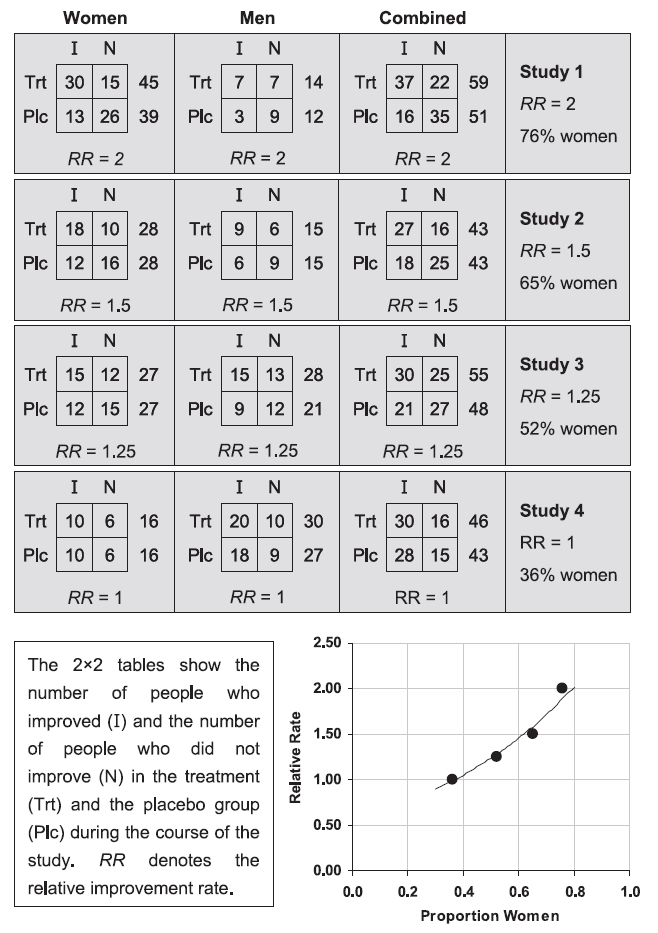
\includegraphics[width=\textwidth]{figBspOekoFehl}
\newline(Quelle: Viechtbauer 2007: 114)
\end{frame}





\section{Publication Bias}\label{sec:pubbias}


\begin{frame}\frametitle{Publication Bias als ein
    \emph{Missing-data}-Problem\protect\footnote{Große Teile dieses Abschnitts
      basieren auf \citet{weis_identification_2011}. }}
  \begin{itemize}
  \item Selbst eine perfekte Literaturrecherche kann nur tatsächlich publizierte Studien finden.
  \item Nichtpublizierte Studien sind dann problematisch, wenn die Gründe für
    die Nichtpublikation mit Eigenheiten der Studien zusammenhängen.
  \item Unter einem \emph{Publication Bias} wird \enquote{the tendency toward
      preparation, submission and publication of research findings based on the
      nature and direction of the research results} \citep[13]{dickersin_publication_2005} verstanden.
  \end{itemize}
\end{frame}


\begin{frame}
  \frametitle{Formen des \emph{Dissemination Bias}}
  %%
  Ein umfassender Begriff, der verschiedene \enquote{information suppression
    mechanisms} einschließt, ist \emph{Dissemination Bias}:
  \begin{itemize}
  \item Publication Bias (nur signifikante, hypothesen-konforme Ergebnisse werden berichtet)
  \item Positive Results Bias
  \item Outcome Bias (selektives Berichten von mehreren möglichen Befunden)
  \item Time-lag-bias, Pipeline Effect
  \item Language Bias
  \item Availability Bias
  \item Cost Bias
  \item Familiarity Bias
  \item \ldots
  \end{itemize}
\end{frame}



\begin{frame}
  \frametitle{Ursachen für Publication Bias}
  %%
  \begin{itemize}
  \item File-drawer-Problematik: Forscher neigen dazu, nicht signifikante oder
    nicht hypothesen-konforme Ergebnisse zurückzuhalten.
  \item Analysen und Modelle werden \enquote{zurechtgebogen} (\emph{model
      tweaking}), um die gewünschten Befunde zu erhalten.
  \item Herausgeber wissenschaftlicher Zeitschriften bevorzugen Studien mit
    signifikanten Ergebnissen.
  \item Dissertationen, Konferenzbeiträge u.ä. werden z.T. nicht veröffentlicht.
  \end{itemize}

  \citep[Für eine theoretische Erörterung möglicher Motive siehe auch][]{auspurg_what_2011}
\end{frame}


\begin{frame}
  \frametitle{Publication Bias \ldots ein wahres Beispiel} "`But reviewers in
  general punish honesty and reward rhetoric. In my own area
  (psycholinguistics), many reviewers (many of them senior researchers who've
  been around for decades) do not even understand basic things in hypothesis
  testing. For example, \alert{an editor-in-chief of a major journal recently
    rejected a paper of mine on the grounds that the p values were not small
    enough below the upper bound of 0.05 (in his words, \glq the effects were
    not strong enough\grq).} If you ask a random researcher what a confidence
  interval is, 95\% will give you the wrong answer; many don't even know what a
  p value tells you (many think it's the probability of the null being false). I
  could go on and on."'  (Shravan Vasishth in
  \url{http://www.stat.columbia.edu/\~cook/movabletype/archives/2007/04/some\_thoughts\_o\_3.html})
\end{frame}


\begin{frame}
  \frametitle{Verfahren zur Identifikation von Publication Bias}

  \begin{itemize}
  \item Funnel Plot
  \item Trim and Fill
  \item \sout{Fail-safe N} (nicht empfohlen!)
  \item Regressions- und Korrelationsverfahren
  \item Selection Models
  \item Caliper Test
  \end{itemize}

  \citep[Quelle: Für eine ausführliche Diskussion der Vor- und Nachteile
  siehe][]{weis_identification_2011, auspurg_what_2011}.

\end{frame}


\begin{frame}
  \frametitle{Identifizierung von PB: Funnel Plot I}
  %%
  Annahme: Es besteht ein Effekt, der klein, aber nicht Null ist.
  \begin{itemize}
  \item Untersuchungen mit kleinen Stichproben weisen eine stärkere
    zufallsbedingte Streuung der Effekte auf; nur die relativ starken Effekte
    sind statistisch signifikant.
  \item Untersuchungen mit großen Stichproben hingegen weisen eher geringe
    Effektstärken auf, die kaum um den wirklichen Wert streuen. Diese relativ
    kleinen Effekte sind aufgrund der großen Stichprobe (meist) signifikant.
  \end{itemize}
  $\rightarrow$ Publikationsverzerrungen liegen vor, wenn kaum Studien
  mit kleinen Stichproben (großer Standardfehler) und geringen Effekten
  publiziert werden und ein "`Loch"' in der Graphik zu erkennen ist.
\end{frame}


\begin{frame}[plain]
  \frametitle{Identifizierung von PB: Funnel Plot II}
  %%
  Ein Funnel Plot wird allgemein nach folgenden Prinzipien konstruiert:
  \begin{itemize}
  \item Auf der X-Achse werden die Effektstärken abgetragen (möglichst mit
    symmetrischer Skala, also log(OR), log(RR) etc.).
  \item Auf der Y-Achse findet sich ein Maß für die Stichprobengröße; meistens
    wird hier der Standardfehler (statt der Fallzahl) der Effektstärken
    verwendet (nach oben hin abnehmend!).
  \item Eine vertikale Linie veranschaulicht den Schätzer des FEM.
  \item Als visuelle Hilfe kann um den Schätzer des FEM pro Einheit des
    Standardfehlers das \emph{erwartete} Konfidenzintervall gezeichnet
    werden. Punkte (95\% innerhalb) außerhalb des entstandenen Trichters weisen
    auf Heterogenität hin.
  \end{itemize}
\end{frame}


\begin{frame}[plain]
  \frametitle{Schematischer Funnel Plot}
  \begin{center}
    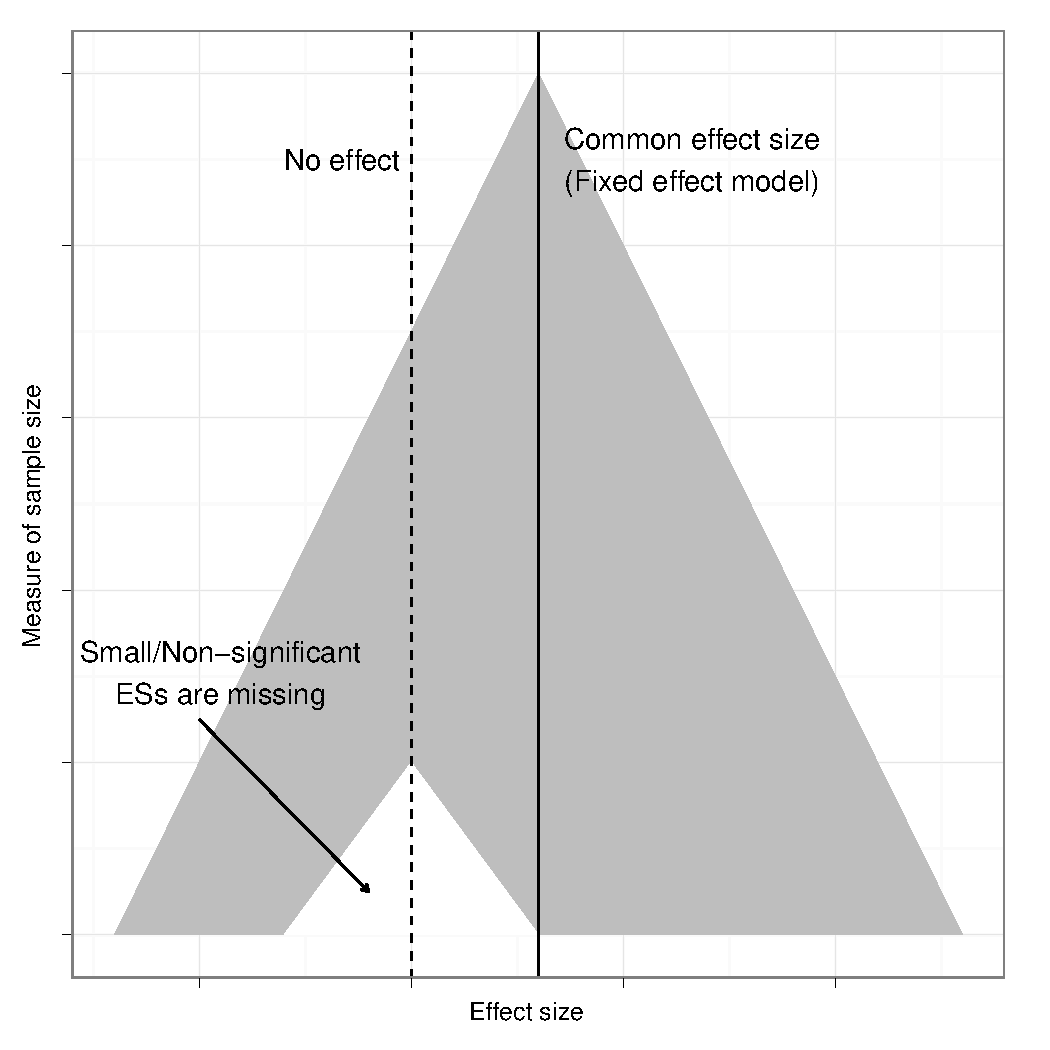
\includegraphics[width=0.65\linewidth]{f_01_schematic_funnelplot}
  \end{center}
  \citep[Quelle: ][666]{weis_identification_2011}
\end{frame}



\begin{frame}[plain]
  \frametitle{Funnel Plot (simulierte Daten)}\label{slide:funnel-sim-data}
  \begin{center}
    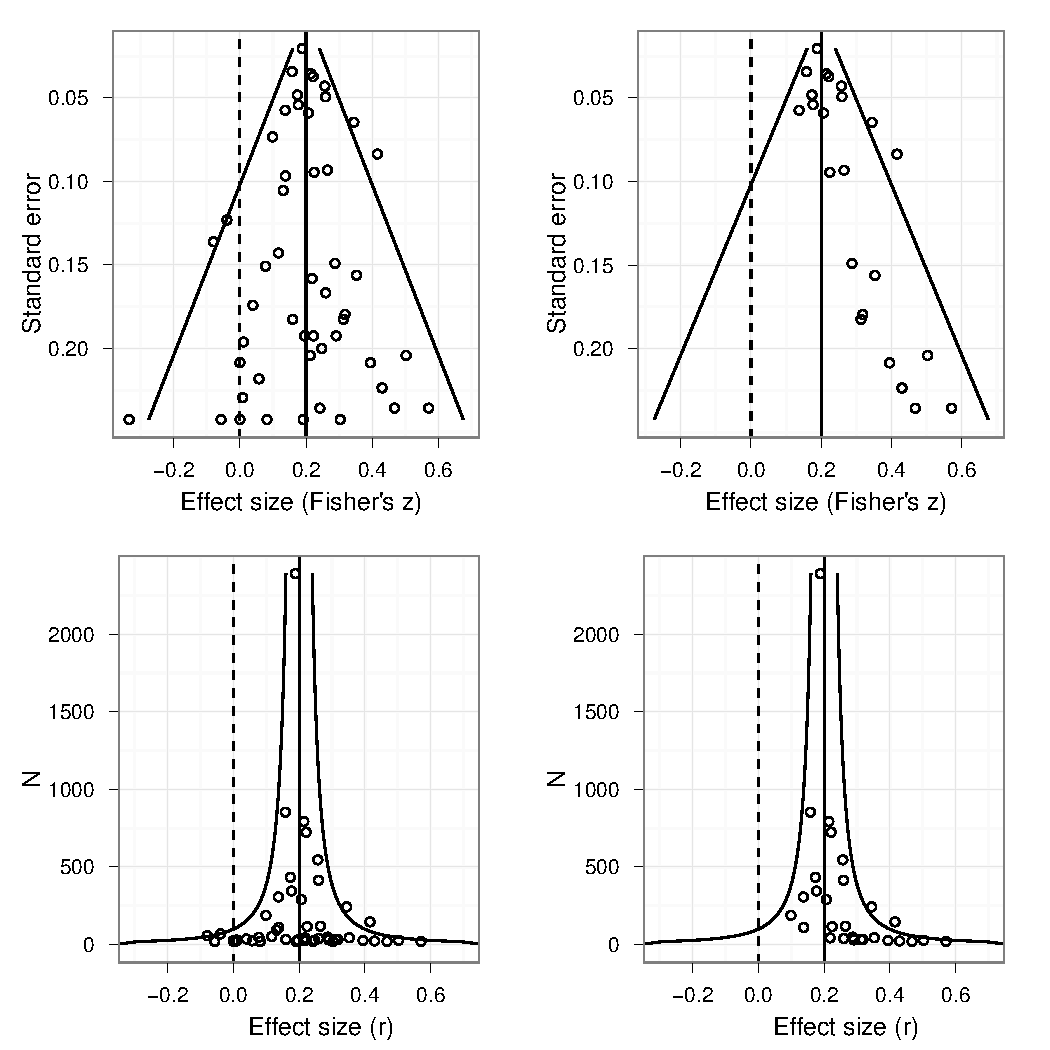
\includegraphics[width=0.68\linewidth]{f_02_FunnelCorrTotal}
  \end{center}
  \citep[Quelle: n.s: $p>0.10$][666]{weis_identification_2011}
\end{frame}



 \begin{frame}
   \frametitle{Trim and Fill}
   \begin{itemize}
   \item Imputationsansatz: Neben den beobachteten $k$ Studien existieren noch
     $k_0$ Studien, die aufgrund des \emph{Publication Bias} nicht ermittelt werden
     konnten.
   \item Aufgabe des Algorithmus ist, die Anzahl und die Ausprägungen dieser
     $k_0$ Studien zu schätzen.
   \item Ein Funnelplot mit den beobachteten und den geschätzten Effektstärken
     vermittelt einen guten Eindruck einer symmetrischen
     Effektstärkenverteilung.
   \item Gleichwohl belegt die Existenz von $k_0$ Studien nicht einen
     \emph{Publication Bias}, es wird erst einmal nur auf eine Asymmetrie der
     Effektstärkenverteilung in Abhängkeit von deren Reliabilität hingewiesen.
   \end{itemize}
 \end{frame}



 \begin{frame}
   \frametitle{Beispiel für Trim and Fill}
   %%
   \begin{center}
     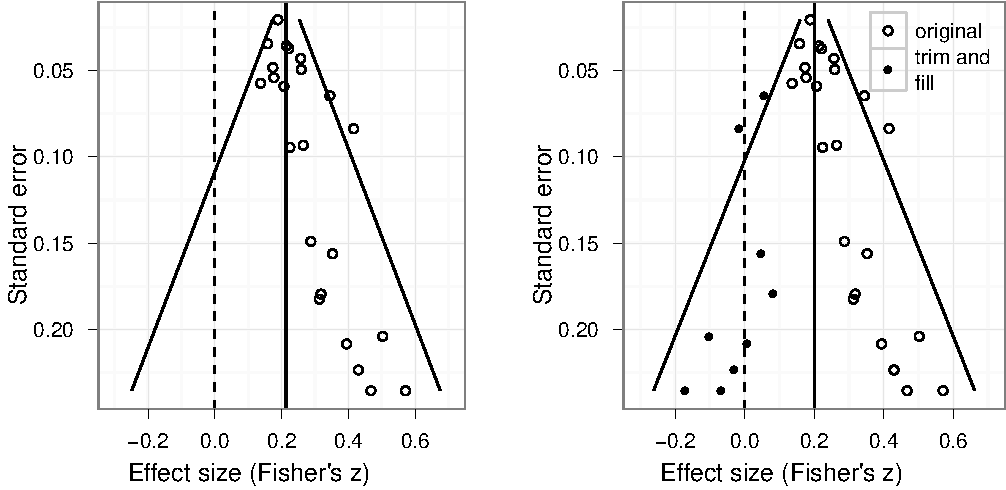
\includegraphics[width=0.92\textwidth]{f_04_FunnelCorrTrimFill}
   \end{center}
   \citep[Quelle: ][671]{weis_identification_2011}.
 \end{frame}



 \begin{frame}
   \frametitle{Korrelationsverfahren}
   Berechnung der Rangkorrelation (Kendall's Rang-Korrelation) zwischen
   (z-standardisierten) Effektstärken und Fehlervarianzen. Ein
   nicht-signifikanter Test deutet auf eine \emph{unverzerrte} Stichprobe hin.
 \end{frame}


  \begin{frame}
   \frametitle{Eggers lineares Regressionsmodell}

   \begin{itemize}
   \item Es wird ein bivariates lineares Regressionsmodell geschätzt.
   \item Als abhängige Variable wird die am Standardfehler normierte
     Effektstärke ($\frac{T_j}{SE_j}$) benutzt.
   \item Das unabhängige Merkmal ist der inverse Standardfehler
     ($\frac{1}{SE_j}$) (\emph{precision}).
   \item Liegt \emph{keine} Verzerrung vor, sollte die Regressionsgerade durch
     den Ursprung laufen ($H_0: \beta_0 = 0$). Warum?:
     \begin{itemize}
     \item $\frac{1}{SE_j}$ nähert sich für kleine Studien 0 (x-Achse).
     \item $\frac{T_j}{SE_j}$ näher sich für kleine Studien auch 0 (y-Achse).
     \end{itemize}

   \end{itemize}
   \citep[Quellen: ][]{egger_bias_1997, sterne_regression_2005}
 \end{frame}


 \begin{frame}[plain, shrink = 5]
   \frametitle{Beispiel für "`Egger's linear regression method"'}
   %%
  \begin{center}
    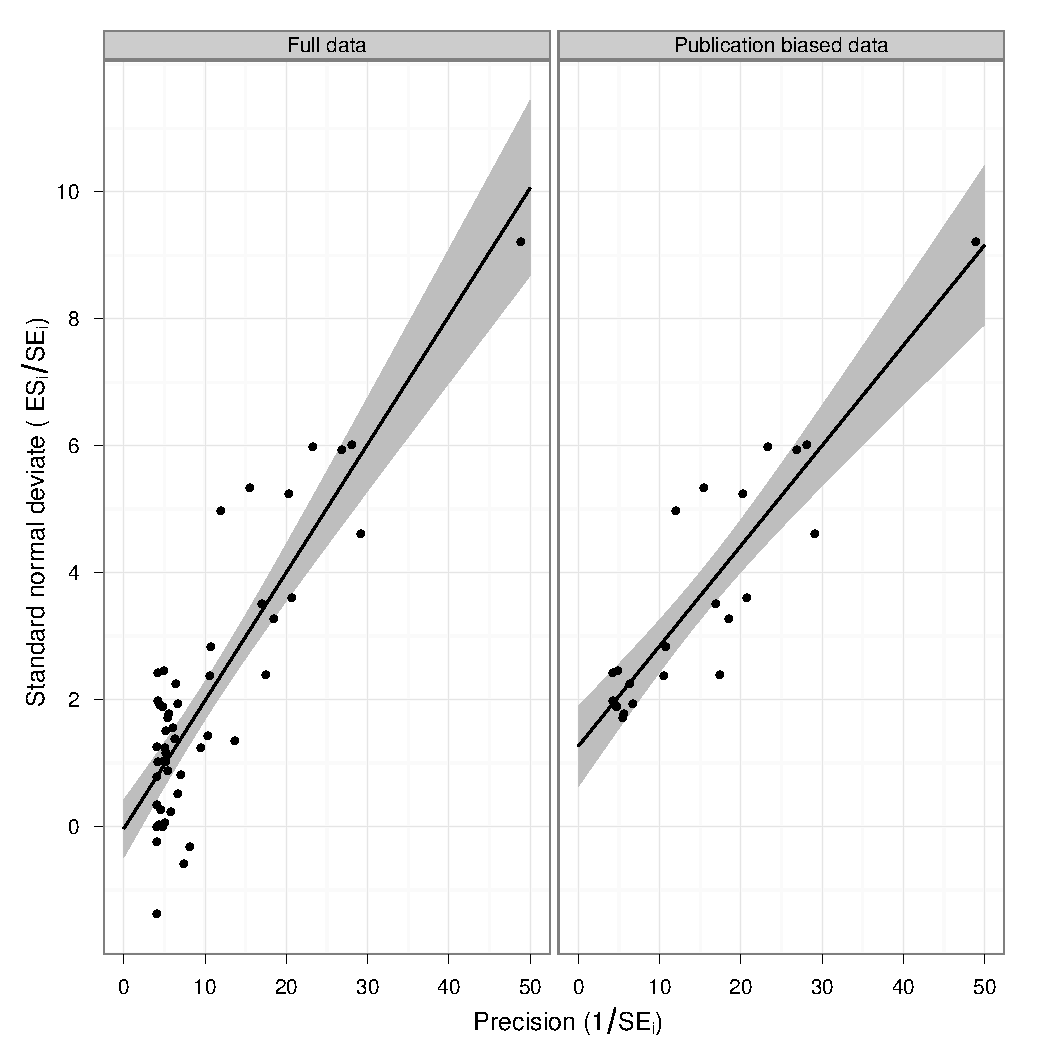
\includegraphics[width=0.91\textheight]{f_03_CompRegPlots}
  \end{center}
  \citep[Quelle: basiert auf simulierten Daten, siehe Folie \pageref{slide:funnel-sim-data};][669]{weis_identification_2011}.
 \end{frame}


\section{Reporting Standards}


\begin{frame}[allowframebreaks]\frametitle{Übersicht Reporting Standards}

  \begin{footnotesize}
    \begin{itemize}
    \item \fullcite{apa_reporting_2008}
    \item \fullcite{stroup_meta-analysis_2000}
    \item \fullcite{liberati_prisma_2009}
    \item \fullcite{riley_meta-analysis_2010}
    \item \fullcite{maer_network_maer_2012}
    \end{itemize}

    (Alle Standards finden sich als PDF-Dateien auch im Verzeichnis
    \texttt{ref/})
  \end{footnotesize}
\end{frame}


\begin{frame}[allowframebreaks]\frametitle{MAER-Net Reporting Standards}
  Quelle: \url{http://www.hendrix.edu/MAER-Network/post.aspx?id=62556&blogid=51160}
  \\ \vspace{1ex}
  MAER-Net (Meta-Analysis of Economics Research (MAER) Network) recommends that
  all meta-analyses in economics should comply with the following reporting
  protocols.

\begin{itemize}
\item Research Questions and Effect Size
  \begin{itemize}
  \item A clear statement of the specific economic theories, hypotheses, or
    effects studied.
  \item A precise definition of how effects are measured (the ‘effect size’),
    accompanied by any relevant formulas.
  \item An explicit description about how measured effects are comparable,
    including any methods used to standardize or convert them to a common
    metric.
  \end{itemize}
\item Research Literature, Searching, Compilation and Coding
  \begin{itemize}
  \item A  full report of how the research literature was searched.  This report should include:
    \begin{itemize}
    \item the exact databases or other sources used;
    \item the precise combination of keywords employed; and
    \item the date that the search was completed.
    \end{itemize}
  \item A full disclosure of the rules for study (or effect size)
    inclusion/exclusion.  It is also useful to provide a list of all studies
    included and a description of why others were excluded.
  \item A statement addressing who searched, read, and coded the research
    literature. Two or more reviewers should code the relevant research.
  \item A complete list of the information coded for each study or estimate. At
    a minimum, we recommend that reviewers code:
    \begin{itemize}
    \item the estimated effect size;
    \item its standard error, when feasible, and the degrees of freedom (or sample size);
    \item variables that distinguish which type of econometric model, methods and techniques were employed;
    \item dummy (i.e., 0/1) variables for the omission of theoretically relevant
      variables in the research study investigated;
    \item empirical setting (e.g., region, market, industry);
    \item data types (panel, cross-sectional, time series, . . . );
    \item year of the data used and/or publication year;
    \item type of publication (journal, working paper, book chapter, etc.); and
    \item the primary study, publication and/or dataset from which an observation is drawn.
    \end{itemize}
  \end{itemize}
\item MRA Modeling Issues
  \begin{itemize}
  \item A table of descriptive statistics of the variables that are coded (means
    and standard deviations) and graph(s) displaying the effect sizes (e.g.,
    funnel graphs, forest plots, bar charts).
  \item A fully reported multiple MRA, along with the exact strategy used to
    simplify it (e.g., general-to-specific, Bayesian).
  \item An investigation of publication, selection, and misspecification biases.
    When suspected, these should be controlled for in subsequent MRA models.
  \item Methods to accommodate heteroscedasticity and within-study dependence.
  \item Results from MRA model specification tests, robustness checks, or sensitivity analyses.
  \end{itemize}

\end{itemize}

With one possible exception, MAER-Net has come to a clear consensus about these
reporting guidelines.  The requirement to have two reviewers code all the
relevant research has received the most comment and discussion.  As economists,
we all are acutely aware of the trade-off between the improved quality that the
second coder will likely add (through catching mistakes and resolving
ambiguities) and the increased cost (in weeks of highly skilled professional
labour). We understand that the highest standards of scientific rigor demand at
least two highly-knowledgeable researchers code the relevant research base.
Nonetheless, MAER-Net does not wish to prohibit Ph.D. students and researchers
at resource-challenged institutions from employing this important tool
to understand their areas of research.  To finesse these opposing concerns, the
above statement is sufficiently broad to encompass a second reviewer randomly
checking a substantial proportion of the research literature if their coding
protocol is stated explicitly and justified.


\end{frame}




\section{Ein Ausblick auf Meta-Analysen mit Individualdaten}

\begin{frame}\frametitle{Was ist eine IPD Meta-Analyse?}

  \begin{quotation}
    \enquote{As with any meta-analysis, an individual participant data meta-analysis aims
    to summarise the evidence on a particular clinical question from multiple
    related studies, such as whether a treatment is effective. The statistical
    implementation of an individual participant data meta-analysis crucially
    \alert{must preserve the clustering of patients within studies}; it is inappropriate
    to simply analyse individual participant data as if they all came from a
    single study. Clusters can be retained during analysis by using a two step
    or a one step approach.}
  \end{quotation}

  \citep[Quelle: ][1]{riley_meta-analysis_2010}

\end{frame}


\begin{frame}\frametitle{APD und IPD Meta-Analysen}
  \begin{itemize}
  \item Meta-Analysen auf der Grundlage von \emph{Aggregate Person Data} (APD)
  \item Meta-Analysen auf der Grundlage von \emph{Individual Person/Participant/Patient Data}
    \begin{itemize}
    \item Einstufige Ansätze: (Mehrebenen-)Regressionsmodelle auf der Grundlage eines gepoolten Datensatzes
    \item Zweistufige Ansätze: pro Datensatz eine Effekstärke berechnen und anschließend eine APD Meta-Analyse durchführen
    \end{itemize}
  \item Meta-Analysen, die sowohl APD und IPD verwenden.
  \end{itemize}
\end{frame}



\begin{frame}\frametitle{Vorteile von IPD Meta-Analysen}
  %%
  \begin{footnotesize}
    \begin{itemize}
    \item Erhöhte Auswahl angemessener Analyseverfahren, etwa für die Analyse
      von nicht-experimentellen Daten (multivariate Auswertungstechniken).
    \item Zentrale Merkmale lassen sich vereinheitlichen, erhöht die
      Vergleichbarkeit der Konstrukte.
    \item Bei zweistufigem Vorgehen keine Probleme mit fehlenden ES-Angaben.
    \item Es lassen sich zusätzliche Hypothesen untersuchen, insbesondere
      solche, die mit individuellen Charakteristika zusammenhängen.
    \item U.U. größere statistische \emph{power}, um Interaktionen zwischen
      Studienmerkmalen und ES zu finden.
    \item Schließlich besteht bei der Verwendung von Aggregatdaten immer die
      Gefahr eines ökologischen Fehlschlusses.
    \end{itemize}
    \citep[Quelle: ][252]{weis_potentiale_2008, pigott_advances_2012}
  \end{footnotesize}
\end{frame}


\begin{frame}\frametitle{Nachteile von IPD Meta-Analysen}
  \begin{itemize}
  \item Hoher Kosten- und Zeitaufwand (vor allem Medizin, teilw. Kooperationen von mehreren dutzend Partnern).
  \item Nicht immer sind \emph{alle} vorhandenen Datensätze auch verfügbar.
  \item Große Datensätze und anspruchsvolle Analyseverfahren können Desktop-PCs überfordern.
  \end{itemize}
\end{frame}


\begin{frame}\frametitle{Eigene Erfahrungen mit einer IPD Meta-Analysen}
  \begin{itemize}
  \item Forschungsprojekt: "`How employment status affects partnership stability: A meta-analysis using longitudinal individual person data"'
  \item 16 Längsschnittdatensätze aufbereiten
  \item Gepoolter Datensatz wird (im "`person-period format"') mehrere Millionen Zeilen umfassen
  \item (Sehr/Zu?) Komplexe Dokumentation zur Datenaufbereitung (diskrete EHA)
  \item Offene Probleme:
    \begin{itemize}
    \item Umgang mit Gewichten
    \item Sehr aufwändige Datenaufbereitung (techn. Infrastruktur, Organisation der Skripte, Dokumentation, \ldots)
    \end{itemize}
  \item \ldots
  \end{itemize}
\end{frame}


\begin{frame}[allowframebreaks]\frametitle{Literatur zu IPD Meta-Analysen}
  \begin{footnotesize}
    \begin{itemize}
    \item \fullcite{stewart_ipd_2002}
    \item \fullcite{simmonds_meta-analysis_2005}
    \item \fullcite{riley_meta-analysis_2007}
    \item \fullcite{sutton_meta-analysis_2008}\footnote{Mit einem Bayesianischen Modell Kombination von IPD und
        APD Meta-Analyse.}
    \item \fullcite{cooper_relative_2009}
    \item \fullcite{curran_integrative_2009}
    \item \fullcite{riley_meta-analysis_2010}
    \item \fullcite{pigott_advances_2012} (insbes. Kapitel 8)
    \end{itemize}
  \end{footnotesize}
\end{frame}


\section{Literatur}

\begin{frame}[allowframebreaks]\frametitle{Literaturempfehlungen und weitere Informationsquellen}

  \begin{footnotesize}
    \begin{itemize}
    \item Literatur
      \begin{itemize}
      \item \fullcite{borenstein_introduction_2009}
      \item \fullcite{lipsey_practical_2001}
      \item \fullcite{cooper_research_2010}
      \item \fullcite{petticrew_systematic_2006}
      \item \fullcite{cooper_handbook_2009}
      \end{itemize}
    \item Zeitschriften
      \begin{itemize}
      \item Research Synthesis Methods
        <\url{http://onlinelibrary.wiley.com/journal/10.1002/\%28ISSN\%291759-2887}>
      \item Statistics in Medicine
        <\url{http://onlinelibrary.wiley.com/journal/10.1002/\%28ISSN\%291097-0258}>
      \item Systematic Reviews <\url{http://www.systematicreviewsjournal.com/}>
      \end{itemize}
    \item Organisationen
      \begin{itemize}
      \item The Cochrane Collaboration <\url{http://www.cochrane.org/}>
      \item The Campbell Collaboration
        <\url{http://www.campbellcollaboration.org/}>
      \end{itemize}
    \end{itemize}
  \end{footnotesize}
\end{frame}

\renewcommand{\bibfont}{\normalfont\tiny}
\begin{frame}[allowframebreaks, plain]\frametitle{Literatur}
\printbibliography
\end{frame}




%%% Local Variables:
%%% TeX-master: "ps2012gesis-ma-workshop.tex"
%%% End:



%%%%33333
\part{Anhang}\label{part:anhang}
\frame{\partpage}

\frame{\frametitle{Anhang}\tableofcontents[part=5, hideallsubsections]}


\section{Meta-Analyse-Software für R und Stata}

\begin{frame}\frametitle{Meta-Analyse-Software für R}
  %%
  R Pakete (sozialwissenschaftliche Auswahl):
  \begin{itemize}
  \item \texttt{meta} (uni- und bivariate Meta-Analyse; mächtiger als \texttt{rmeta})
  \item \texttt{rmeta} (univariate Meta-Analyse)
  \item \texttt{metafor} (Meta-Regression; sehr umfangreich, siehe auch \url{http://www.metafor-project.org/})
  \item \texttt{mvmeta} (Multivariate Meta-Analyse)
  \item \texttt{metacor}
  \item \texttt{MAc}, \texttt{MAclinical}, \texttt{MAd} (für eine Einführung
    siehe
    \url{http://rwiki.sciviews.org/doku.php?id=packages:cran:ma_meta-analysis})
  \item \texttt{compute.es} (zur Berechnung und Konvertierung von Effektstärken)
  \end{itemize}
\end{frame}



\begin{frame}\frametitle{Meta-Analyse-Software Stata}

  \begin{itemize}
  \item Eine Liste von Stata add-ons ist unter
    \url{http://www.stata.com/support/faqs/statistics/meta-analysis/} (What
    meta-analysis features are available in Stata?) verfügbar.
  \item \citet{sterne_meta-analysis_2009} hat \enquote{Meta-Analysis in Stata:
      An Updated Collection from the Stata Journal} herausgegeben.
  \end{itemize}
\end{frame}




\begin{frame}\frametitle{Sonstige Meta-Analyse-Software}
  \begin{itemize}
   \item SPSS: "`meta-analysis stuff"' von David B. Wilson (\url{http://mason.gmu.edu/~dwilsonb/ma.html})
   \item Comprehensive Meta-Analysis: \url{http://www.meta-analysis.com/}
   \item OpenMeta[Analyst]: \url{http://tuftscaes.org/open_meta/} (interessant,
     basiert auf R und verwendet u.a. \texttt{metafor})
  \item \ldots
  \end{itemize}
\end{frame}




\section{R in 20 Minuten}

\begin{frame}[plain]\frametitle{Grundlagen von R}
  \begin{footnotesize}
    \begin{itemize}
    \item R ist ein Statistikprogramm \emph{und} eine Programmiersprache <\url{http://www.r-project.org/}>.
    \item (Fast) Alles in R sind \emph{Objekte} (etwa Datensätze oder Ergebnisse
      von Berechnungen).
    \item Sofern der Hauptspeicher ausreicht, können dort beliebig viele R
      Objekte \emph{gleichzeitig} existieren (d.h. auch mehrere Datensätze).
    \item Das Laden von Datensätzen oder Speichern von Ergebnissen ist daher
      \emph{immer} mit einer Zuweisung (\emph{assignment}) (R-Befehl: \lstinline|<-|)
      verbunden.
    \item R ist modular aufgebaut. Bestimmte (statistische) Funktionen
      (Meta-Analyse, Mehrebenenmodelle, Überlebensmodelle etc.) müssen erst (via
      \code{library(Paketname)} geladen werden.
    \item R ist \emph{case sensitive}, d.h. \texttt{mean(x)} $\neq$ \texttt{Mean(x)}.
    \item Unter MS Windows werden in R für Dateipfade immer \emph{slashes} (/)
      verwendet, \emph{backslash} ($\backslash$) ist nur als doppelter
      \emph{backslash} ($\backslash\backslash$) erlaubt.
    \item R ist streng im Umgang mit fehlenden Werten (mit \code{NA}
      gekennzeichnet) und bpsw. muss in vielen Funktionen ein listenweiser Ausschluss ausdrücklich angegeben werden.
    \item Kommentare werden mit dem Zeichen \# eingeleitet.
    \end{itemize}
  \end{footnotesize}
\end{frame}





\begin{frame}[fragile]\frametitle{Zuweisungen und R Ausgabe}

  Zuweisungen erfolgen in R mit dem Befehl \code{<-}:




\begin{knitrout}
\definecolor{shadecolor}{rgb}{0.827, 0.827, 0.827}\color{fgcolor}\begin{kframe}
\begin{alltt}
x <- 22
x
\end{alltt}
\begin{verbatim}
R> [1] 22
\end{verbatim}
\end{kframe}
\end{knitrout}


Mit \code{R>} wird hier die R-Ausgabe bezeichnet. \code{[1]} kennzeichnet in R das
i-te Elemente in der jeweiligen Zeile (hier, nur 1 Element).

\begin{knitrout}
\definecolor{shadecolor}{rgb}{0.827, 0.827, 0.827}\color{fgcolor}\begin{kframe}
\begin{alltt}
y <- 1:15
y
\end{alltt}
\begin{verbatim}
R>  [1]  1  2  3  4  5  6  7  8  9 10 11 12
R> [13] 13 14 15
\end{verbatim}
\end{kframe}
\end{knitrout}


\end{frame}



\begin{frame}[fragile, plain]\frametitle{R als Taschenrechner}
\begin{footnotesize}
\begin{knitrout}
\definecolor{shadecolor}{rgb}{0.827, 0.827, 0.827}\color{fgcolor}\begin{kframe}
\begin{alltt}
\hlcomment{## Mit Skalaren rechnen}
x <- 123
y <- 7
x + y
\end{alltt}
\begin{verbatim}
R> [1] 130
\end{verbatim}
\begin{alltt}

\hlcomment{## Mit Vektoren (= Variablen) rechnen}
\hlcomment{## c() erzeugt einen Vektor (c = concatenate)}
x <- \hlfunctioncall{c}(3, 6, 9)
x
\end{alltt}
\begin{verbatim}
R> [1] 3 6 9
\end{verbatim}
\begin{alltt}
y <- x/3
y
\end{alltt}
\begin{verbatim}
R> [1] 1 2 3
\end{verbatim}
\end{kframe}
\end{knitrout}

\end{footnotesize}
\end{frame}



\begin{frame}\frametitle{Wichtige Funktionen}
  \begin{itemize}
  \item Hilfeseiten aufrufen: \code{help(Funktionsname)} oder
    \code{?Funktionsname} (Bsp.: \code{help(mean)} oder \code{?mean})
  \item Welche Objekte sind im \emph{workspace}: \code{ls()}
  \item Arbeitsverzeichnis definieren/abfragen: \code{setwd("Pfad")} und \code{getwd()}
  \item Beschreibung eines R-Objektes: \code{str(Robjekt)}
  \item (Variablen-)Namen eines R-Objektes: \code{names(Robjekt)}
  \item Die ersten n Fälle anzeigen: \code{head(Robjekt)}
  \end{itemize}
\end{frame}


\begin{frame}[plain, fragile, shrink=10]\frametitle{Hilfeausgabe für \code{?mean}}

\begin{tiny}
\begin{verbatim}
mean                   package:base                    R Documentation

Arithmetic Mean

Description:

     Generic function for the (trimmed) arithmetic mean.

Usage:

     mean(x, ...)

     ## Default S3 method:
     mean(x, trim = 0, na.rm = FALSE, ...)

Arguments:

       x: An R object.  Currently there are methods for numeric/logical
          vectors and date, date-time and time interval objects, and
          for data frames all of whose columns have a method.  Complex
          vectors are allowed for ‘trim = 0’, only.

    trim: the fraction (0 to 0.5) of observations to be trimmed from
          each end of ‘x’ before the mean is computed.  Values of trim
          outside that range are taken as the nearest endpoint.

   na.rm: a logical value indicating whether ‘NA’ values should be
          stripped before the computation proceeds.

     ...: further arguments passed to or from other methods.

Value:

     If ‘trim’ is zero (the default), the arithmetic mean of the values
     in ‘x’ is computed, as a numeric or complex vector of length one.
     If ‘x’ is not logical (coerced to numeric), numeric (including
     integer) or complex, ‘NA_real_’ is returned, with a warning.

     If ‘trim’ is non-zero, a symmetrically trimmed mean is computed
     with a fraction of ‘trim’ observations deleted from each end
     before the mean is computed.

References:

     Becker, R. A., Chambers, J. M. and Wilks, A. R. (1988) _The New S
     Language_.  Wadsworth & Brooks/Cole.

See Also:

     ‘weighted.mean’, ‘mean.POSIXct’, ‘colMeans’ for row and column
     means.

Examples:

     x <- c(0:10, 50)
     xm <- mean(x)
     c(xm, mean(x, trim = 0.10))
\end{verbatim}
\end{tiny}
\end{frame}



\begin{frame}[fragile]\frametitle{Daten laden und untersuchen I}
\begin{footnotesize}



\begin{knitrout}
\definecolor{shadecolor}{rgb}{0.827, 0.827, 0.827}\color{fgcolor}\begin{kframe}
\begin{alltt}
\hlcomment{## Zuweisung nicht vergessen!}
dat <- \hlfunctioncall{read.csv}(file = \hlstring{"../../data/dVerbAb.csv"},
                sep = \hlstring{";"}, dec = \hlstring{","})

\hlcomment{## head() zeigt die ersten 6 Zeilen eines}
\hlcomment{## R Objektes an}
\hlfunctioncall{head}(dat)
\end{alltt}
\begin{verbatim}
R>   ID year pub     r   N      Var      SE
R> 1  1 1980   0 -0.10   7 0.163350 0.40417
R> 2  2 2005   1  0.23  76 0.011960 0.10936
R> 3  4 1968   0 -0.05 155 0.006461 0.08038
R> 4  5 1968   0  0.02  45 0.022709 0.15070
R> 5  6 1969   1 -0.09  31 0.032796 0.18110
R> 6  7 1969   1  0.26  37 0.024149 0.15540
\end{verbatim}
\end{kframe}
\end{knitrout}

\end{footnotesize}
\end{frame}


\begin{frame}[fragile, plain]\frametitle{Daten laden und untersuchen II}
\begin{tiny}

\begin{knitrout}
\definecolor{shadecolor}{rgb}{0.827, 0.827, 0.827}\color{fgcolor}\begin{kframe}
\begin{alltt}
\hlcomment{## Struktur anzeigen}
\hlfunctioncall{str}(dat)
\end{alltt}
\begin{verbatim}
R> 'data.frame':	17 obs. of  7 variables:
R>  $ ID  : int  1 2 4 5 6 7 9 10 11 12 ...
R>  $ year: int  1980 2005 1968 1968 1969 1969 1970 1987 1987 1993 ...
R>  $ pub : int  0 1 0 0 1 1 0 1 1 1 ...
R>  $ r   : num  -0.1 0.23 -0.05 0.02 -0.09 0.26 -0.07 0.04 -0.01 0.12 ...
R>  $ N   : int  7 76 155 45 31 37 79 151 151 64 ...
R>  $ Var : num  0.16335 0.01196 0.00646 0.02271 0.0328 ...
R>  $ SE  : num  0.4042 0.1094 0.0804 0.1507 0.1811 ...
\end{verbatim}
\begin{alltt}

\hlcomment{## Dimensionen}
\hlfunctioncall{dim}(dat)
\end{alltt}
\begin{verbatim}
R> [1] 17  7
\end{verbatim}
\begin{alltt}

\hlcomment{## Variablennamen ausgeben lassen}
\hlfunctioncall{names}(dat)
\end{alltt}
\begin{verbatim}
R> [1] "ID"   "year" "pub"  "r"    "N"    "Var" 
R> [7] "SE"
\end{verbatim}
\end{kframe}
\end{knitrout}

\end{tiny}
\end{frame}


\begin{frame}[fragile]\frametitle{Mit Datenobjekten (data.frame) arbeiten I}
\begin{footnotesize}
\begin{knitrout}
\definecolor{shadecolor}{rgb}{0.827, 0.827, 0.827}\color{fgcolor}\begin{kframe}
\begin{alltt}
\hlcomment{## Einzelne Elemente eines data.frame}
\hlcomment{## ansprechen: mit $}
dat$r
\end{alltt}
\begin{verbatim}
R>  [1] -0.10  0.23 -0.05  0.02 -0.09  0.26 -0.07
R>  [8]  0.04 -0.01  0.12  0.03  0.07 -0.05  0.13
R> [15]  0.03  0.21  0.28
\end{verbatim}
\begin{alltt}

\hlcomment{## Einzelne Elemente des data.frame}
\hlcomment{## ansprechen: Indexnotation}
dat[, \hlstring{"r"}]
\end{alltt}
\begin{verbatim}
R>  [1] -0.10  0.23 -0.05  0.02 -0.09  0.26 -0.07
R>  [8]  0.04 -0.01  0.12  0.03  0.07 -0.05  0.13
R> [15]  0.03  0.21  0.28
\end{verbatim}
\end{kframe}
\end{knitrout}

\end{footnotesize}
\end{frame}


\begin{frame}[fragile]\frametitle{Mit Datenobjekten (data.frame) arbeiten II}
\begin{footnotesize}
\begin{knitrout}
\definecolor{shadecolor}{rgb}{0.827, 0.827, 0.827}\color{fgcolor}\begin{kframe}
\begin{alltt}
\hlcomment{## Mehrere Elemente eines data.frame}
\hlcomment{## ansprechen: nur noch Indexnotation}
\hlcomment{## Fälle 1:5, Variablen: r und Var}
dat[1:5, \hlfunctioncall{c}(\hlstring{"r"}, \hlstring{"Var"})]
\end{alltt}
\begin{verbatim}
R>       r      Var
R> 1 -0.10 0.163350
R> 2  0.23 0.011960
R> 3 -0.05 0.006461
R> 4  0.02 0.022709
R> 5 -0.09 0.032796
\end{verbatim}
\end{kframe}
\end{knitrout}

\end{footnotesize}
\end{frame}


\begin{frame}[fragile, plain]\frametitle{Deskriptive Statistik}
\begin{footnotesize}
\begin{knitrout}
\definecolor{shadecolor}{rgb}{0.827, 0.827, 0.827}\color{fgcolor}\begin{kframe}
\begin{alltt}
\hlfunctioncall{summary}(dat[, \hlfunctioncall{c}(\hlstring{"r"}, \hlstring{"pub"})])
\end{alltt}
\begin{verbatim}
R>        r                pub       
R>  Min.   :-0.1000   Min.   :0.000  
R>  1st Qu.:-0.0500   1st Qu.:0.000  
R>  Median : 0.0300   Median :1.000  
R>  Mean   : 0.0618   Mean   :0.706  
R>  3rd Qu.: 0.1300   3rd Qu.:1.000  
R>  Max.   : 0.2800   Max.   :1.000
\end{verbatim}
\begin{alltt}
\hlfunctioncall{sd}(dat$r)
\end{alltt}
\begin{verbatim}
R> [1] 0.1241
\end{verbatim}
\begin{alltt}
\hlfunctioncall{table}(dat$pub)
\end{alltt}
\begin{verbatim}
R> 
R>  0  1 
R>  5 12
\end{verbatim}
\end{kframe}
\end{knitrout}

\end{footnotesize}
\end{frame}



\begin{frame}[fragile]\frametitle{Einen Teildatensatz erstellen}\framesubtitle{SPSS/Stata: \code{if}}
\begin{footnotesize}
\begin{knitrout}
\definecolor{shadecolor}{rgb}{0.827, 0.827, 0.827}\color{fgcolor}\begin{kframe}
\begin{alltt}
\hlfunctioncall{subset}(dat, pub==0)
\end{alltt}
\begin{verbatim}
R>    ID year pub     r   N      Var      SE
R> 1   1 1980   0 -0.10   7 0.163350 0.40417
R> 3   4 1968   0 -0.05 155 0.006461 0.08038
R> 4   5 1968   0  0.02  45 0.022709 0.15070
R> 7   9 1970   0 -0.07  79 0.012695 0.11267
R> 11 13 1991   0  0.03 318 0.003149 0.05612
\end{verbatim}
\begin{alltt}
\hlfunctioncall{subset}(dat, pub==0 & r > 0)
\end{alltt}
\begin{verbatim}
R>    ID year pub    r   N      Var      SE
R> 4   5 1968   0 0.02  45 0.022709 0.15070
R> 11 13 1991   0 0.03 318 0.003149 0.05612
\end{verbatim}
\end{kframe}
\end{knitrout}

\end{footnotesize}
\end{frame}



\begin{frame}[fragile]\frametitle{Bedingtes Recodieren}
\begin{footnotesize}
\begin{knitrout}
\definecolor{shadecolor}{rgb}{0.827, 0.827, 0.827}\color{fgcolor}\begin{kframe}
\begin{alltt}
\hlcomment{## Kopie erstellen}
tmp <- dat
tmp$pub
\end{alltt}
\begin{verbatim}
R>  [1] 0 1 0 0 1 1 0 1 1 1 0 1 1 1 1 1 1
\end{verbatim}
\begin{alltt}

\hlcomment{## pub == 0 mit 99 ersetzen}
tmp$pub <- \hlfunctioncall{ifelse}(tmp$pub == 0, 99, tmp$pub)
tmp$pub
\end{alltt}
\begin{verbatim}
R>  [1] 99  1 99 99  1  1 99  1  1  1 99  1  1  1  1
R> [16]  1  1
\end{verbatim}
\end{kframe}
\end{knitrout}

\end{footnotesize}
\end{frame}


\begin{frame}[fragile, plain, shrink]\frametitle{Umgang mit Missings}
\begin{footnotesize}
\begin{knitrout}
\definecolor{shadecolor}{rgb}{0.827, 0.827, 0.827}\color{fgcolor}\begin{kframe}
\begin{alltt}
\hlcomment{## Kopie erstellen}
tmp <- dat
\hlcomment{## 0 wird zu missing (NA)}
tmp$pub <- \hlfunctioncall{ifelse}(tmp$pub == 0, NA, tmp$pub)

\hlcomment{## subset nur missings in pub}
\hlfunctioncall{subset}(tmp, \hlfunctioncall{is.na}(pub))
\end{alltt}
\begin{verbatim}
R>    ID year pub     r   N      Var      SE
R> 1   1 1980  NA -0.10   7 0.163350 0.40417
R> 3   4 1968  NA -0.05 155 0.006461 0.08038
R> 4   5 1968  NA  0.02  45 0.022709 0.15070
R> 7   9 1970  NA -0.07  79 0.012695 0.11267
R> 11 13 1991  NA  0.03 318 0.003149 0.05612
\end{verbatim}
\begin{alltt}

\hlcomment{## is.na-Funktion}
\hlfunctioncall{is.na}(tmp$pub)
\end{alltt}
\begin{verbatim}
R>  [1]  TRUE FALSE  TRUE  TRUE FALSE FALSE  TRUE
R>  [8] FALSE FALSE FALSE  TRUE FALSE FALSE FALSE
R> [15] FALSE FALSE FALSE
\end{verbatim}
\end{kframe}
\end{knitrout}

\end{footnotesize}
\end{frame}




\begin{frame}[plain]\frametitle{RStudio und R}
  \begin{itemize}
  \item Unter MS-Windows gibt es zur Bedienung von R nur die spartanische R Console.
  \item Empfehlenswert ist RStudio, eine kostenlose integrierte
    Entwicklungsumgebung für R <\url{http://www.rstudio.com/ide/}>.
  \end{itemize}
  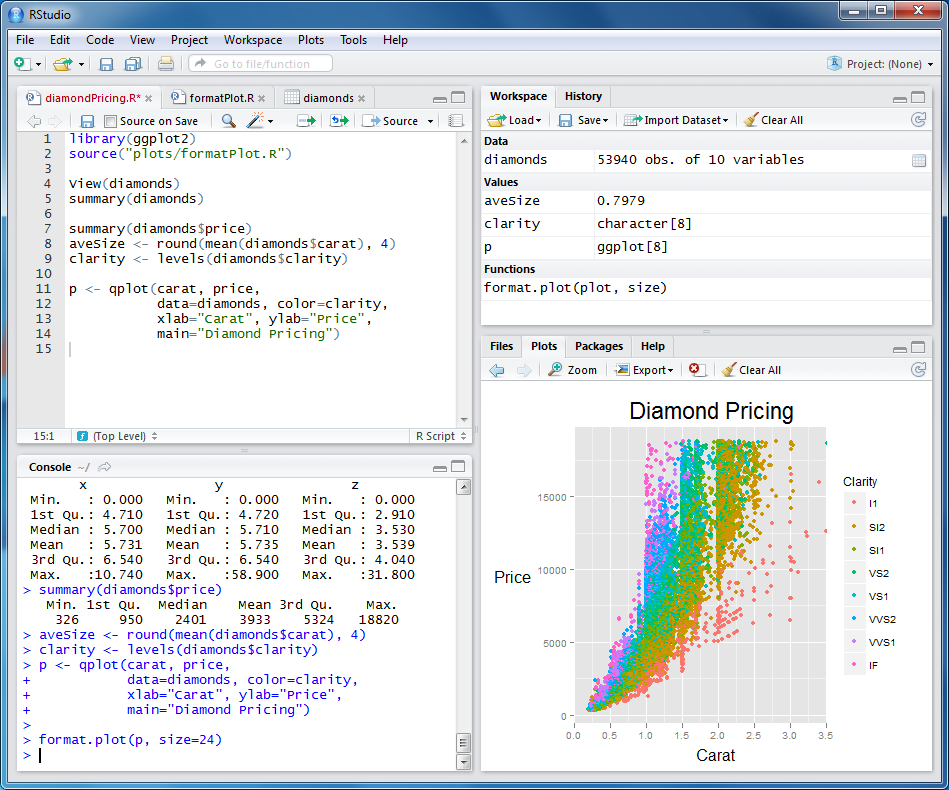
\includegraphics[width=0.7\textwidth]{rstudio-windows.png}
\end{frame}


\section{Statistische Grundlagen}


\subsection{Der Standardfehler}\label{sec:der-standardfehler}

\begin{frame}
  \frametitle{Was ist Inferenzstatistik?}
  \begin{itemize}
  \item<+-> Inferenzstatistik befasst sich mit dem Schluss von der Stichprobe auf die Grundgesamtheit (Population).
  \item<+-> Dieser Schluss ist (immer) fehlerbehaftet; neben dem Schätzen des Populationsparameters ("`Punktschätzung"') ist daher von
    zentraler Bedeutung, die Unsicherheit bei der Parameterschätzung beschreiben zu können.
  \item<+-> Der \emph{Standardfehler} ist ein Streuungsmaß, das die Unsicherheit der Parameterschätzung beschreibt.
  \item<+-> Mit Hilfe des Standardfehlers lässt sich das Konfidenzintervall ("`Intervallschätzung"') berechnen sowie die
    Irrtumswahrscheinlichkeit bestimmen.
  \end{itemize}
\end{frame}


\begin{frame}
  \frametitle{Der Standardfehler für das arithmetische Mittel}
  \begin{itemize}
      \item Der SE beschreibt die Güte des ermittelten Stichprobenwertes: Je größer die Fallzahl, desto kleiner der
    SE. Je kleiner der Standardfehler, desto besser die Schätzung.
  \item Der Standardfehler (SE) des Stichprobenmittelwertes lautet:
    \begin{equation*}
      \frac{\text{Standardabweichung des Merkmals}}{\sqrt{\text{Fallzahl}}}=\frac{\sigma}{\sqrt{N}}.
    \end{equation*}
  \item Der SE gibt die Streuung der Stichproben-Mittelwerte von gleichgroßen und zufällig aus einer Grundgesamtheit gezogenen
    Stichproben um den wahren Populationsmittelwert $\mu$ (sprich "`mü"'; allgemein: $\theta$, sprich: theta) an.
  \end{itemize}
\end{frame}

\subsection{Wahrscheinlichkeitsverteilungen und Q-Test}


\begin{frame}
  \frametitle{Exkurs: Die statistische Beschreibung von Wahrscheinlichkeitsverteilungen}
  Die folgenden Ausführungen zur statistischen Signifikanz von Q verweisen (teilweise implizit, teilweise explizit) auf
  die Beschreibung der Wahrscheinlichkeitsverteilung einer Zufallsvariablen. Die folgenden Begriffe sollten Sie ggf. noch einmal auffrischen:
  \begin{itemize}
  \item Diskrete Zufallsvariablen: Wahrscheinlichkeitsfunktion; stetige Zufallsvariablen:
    Wahrscheinlichkeitsdichtefunktion (teilw. mit "`Dichte"' abgekürzt; engl.: \emph{probability density function})
  \item Mit Hilfe von Wahrscheinlichkeitsverteilungen lassen sich Ereignissen Wahrscheinlichkeiten zuordnen.
  \item (Kumulative) Verteilungsfunktion
  \item Quantilfunktion
  \end{itemize}
\end{frame}



\begin{frame}
  \frametitle{Idee des $Q$-Tests (I)}
  %%
  \begin{itemize}
  \item $Q$ ist die Gesamtvariation (nicht -varianz!) (beobachtete Variation), $df = k-1$ die erwartete Variation im
    Falle des FEM (es gibt \emph{einen gemeinsamen} Populationsparameter) und $Q-k-1$ die Abweichung zwischen
    beobachteter und erwarteter Variation.
  \item Wenn $Q \leq df$ gilt, dann wird definitionsgemäß $Q=0$ und es wird eine homogene Effektstärkenverteilung
    unterstellt.
  \item Wenn aber $Q > df$ ($Q-df > 0$) gilt, müssen wir dann \emph{immer} von einer heterogenen ES-Verteilung ausgehen? Oder
    muss $Q$ ($Q-df$) nicht "'ziemlich groß sein"', damit die Idee einer homogenen Effektstärkenverteilung zurückgewiesen
    werden kann? Was aber heißt "`ziemlich groß"'?
  \end{itemize}
\end{frame}


\begin{frame}[plain]
  \frametitle{Idee des $Q$-Tests (II)}
  %%
  \begin{small}
    \begin{itemize}
    \item Der $Q$-Wert folgt einer sogenannten $\chi^2$-Verteilung (gehört zu den stetigen
      Wahrscheinlichkeitsverteilungen).
    \item Mit dem Wissen, dass $Q$ $\chi^2$-verteilt ist, lässt sich für einen gegebenen Freiheitsgrad ($df$) bspw. die
      Wahrscheinlichkeit $Pr(0 \leq Q)$ bestimmten, d.h., dass ein bestimmter $Q$-Wert im Intervall $[0, Q]$ liegt. Die
      Wahrscheinlichkeit, dass $Q$ außerhalb des Intervalls liegt (also größer als $Q$ ist bzw. $(Q; +\infty]$), beträgt
      $1-Pr(0 \leq Q)$. Anders formuliert: $1-Pr(0 \leq Q)$ ist die Wahrscheinlichkeit, einen Wert größer als $Q$ zu bekommen.
    \item "`Ziemlich groß"' (siehe vorherige Folie) ist ein $Q$-Wert aber doch dann, wenn $1-Pr(0 \leq Q)$ (= p-Wert =
      Irrtumswahrscheinlichkeit) klein ist, wobei
      verschiedene "`Kleinheitsgrade"' (10\%, 5\%, 1\% = Signifikanzniveaus) unterschieden werden. Zu jedem dieser
      Signifikanzniveaus lässt sich ein theoretischer $\chi^2$-Wert berechnen und wenn der empirische $\chi^2$-Wert (als
      $Q$) größer ist, dann sagen wir, dass der Wert signifikant auf dem 10\%-, 5\%-, 1\%-Niveau ist.
    \item Üblicherweise wird in der Meta-Analyse-Literatur das 10\%-Niveau angenommen.
    \end{itemize}
  \end{small}
\end{frame}


\begin{frame}[fragile, plain]
  \frametitle{Bestimmung der Irrtumswahrscheinlichkeit von $Q$}
  %%
\begin{footnotesize}
Mit R lässt sich für verschiedene Wahrscheinlichkeitsverteilungen die Wahrscheinlichkeit $Pr(X \leq x)$ (= F(x) =
kumulative Verteilungsfunktion) bestimmten -- und nur diese. Da im Falle des Q-Testes aber $1-Pr(0 \leq Q)$ = p-Wert
gesucht wird, muss folglich immer $1-Pr(0 \leq
Q)$ gerechnet werden.

%%berechnungChisq, keep.source = TRUE
\begin{knitrout}
\definecolor{shadecolor}{rgb}{0.827, 0.827, 0.827}\color{fgcolor}\begin{kframe}
\begin{alltt}
\hlcomment{## Q = 10 (df = 5)}
1-\hlfunctioncall{pchisq}(q = 10, df = 5)
\end{alltt}
\begin{verbatim}
R> [1] 0.07524
\end{verbatim}
\begin{alltt}

\hlcomment{## Q = 36.1437 (df = 5), Borenstein Tab 14.7}
1-\hlfunctioncall{pchisq}(q = 36.1437, df = 5)
\end{alltt}
\begin{verbatim}
R> [1] 8.89e-07
\end{verbatim}
\begin{alltt}

\hlcomment{## Welches Q fuer alpha <= 0.1?}
\hlfunctioncall{qchisq}(0.9, df  = 5)
\end{alltt}
\begin{verbatim}
R> [1] 9.236
\end{verbatim}
\end{kframe}
\end{knitrout}

\end{footnotesize}
\end{frame}


\begin{frame}[shrink = 5]
  \frametitle{Quantile der $\chi^2-Verteilung$ (df = 3)}
  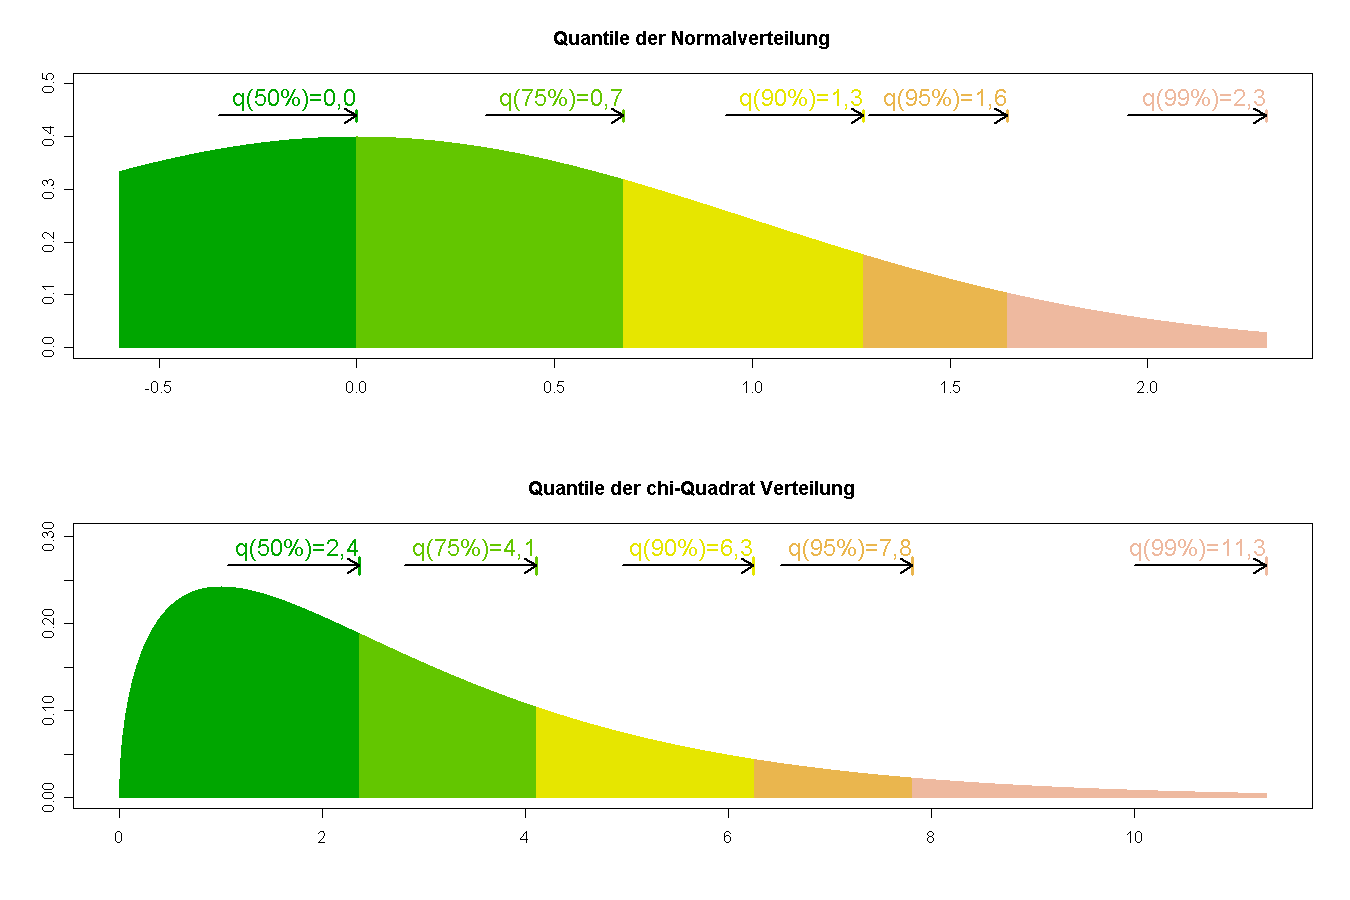
\includegraphics[width=0.9\textwidth]{Quantile_graph}
\newline(Quelle: \url{http://de.wikipedia.org/wiki/Chi-Quadrat-Verteilung})
\end{frame}





%%% Local Variables:
%%% mode: latex
%%% TeX-master: "ps2012gesis-ma-workshop.Rnw"
%%% End:





\end{document}

%%% Local Variables:
%%% TeX-master: "ps2012gesis-ma-workshop.Rnw"
%%% End:
